%%%%%%%%%%%%%%%%%%%%%%%%%%%%%%%%%%%%%%%%%
% Thin Sectioned Essay
% LaTeX Template
% Version 1.0 (3/8/11)
%
% This template has been downloaded from:
% http://www.LaTeXTemplates.com
%
% Original Author:
% Nicolas Diaz (nsdiaz@uc.cl) with extensive modifications by:
% Vel (vel@latextemplates.com)
%
% License:
% CC BY-NC-SA 3.0 (http://creativecommons.org/licenses/by-nc-sa/3.0/)
%
%%%%%%%%%%%%%%%%%%%%%%%%%%%%%%%%%%%%%%%%%

%----------------------------------------------------------------------------------------
%	PACKAGES AND OTHER DOCUMENT CONFIGURATIONS
%----------------------------------------------------------------------------------------

\documentclass[a4paper, 11pt]{article} % Font size (can be 10pt, 11pt or 12pt) and paper size (remove a4paper for US letter paper)
\usepackage{hyperref}

\usepackage[protrusion=true,expansion=true]{microtype} % Better typography
\usepackage{graphicx} % Required for including pictures
\usepackage{wrapfig} % Allows in-line images
\usepackage{tablefootnote} % to display footnotes in tables
\usepackage{threeparttable}
\usepackage[toc,page]{appendix}
\usepackage{multirow}
\usepackage{color}

\usepackage{mathpazo} % Use the Palatino font
\usepackage[T1]{fontenc} % Required for accented characters
\linespread{1.05} % Change line spacing here, Palatino benefits from a slight increase by default


% SPECIAL COMMANDS  

\newcommand{\hls}{HLS\,J0918+5142}
\makeatletter
%\renewcommand\@biblabel[1]{\textbf{#1.}} % Change the square brackets for each bibliography item from '[1]' to '1.'
\renewcommand{\@listI}{\itemsep=0pt} % Reduce the space between items in the itemize and enumerate environments and the bibliography

% TITLE

\renewcommand{\maketitle}{ % Customize the title - do not edit title and author name here, see the TITLE block below
\begin{flushleft} % Right align
{\LARGE\@title} % Increase the font size of the title

\vspace{50pt} % Some vertical space between the title and author name

{\large\@author} % Author name
\\\@date % Date

\vspace{40pt} % Some vertical space between the author block and abstract
\end{flushleft}
}

%
% PAGE STYLE
%
\setlength{\textwidth}{16cm}
\setlength{\textheight}{23cm}
\oddsidemargin +0.5cm
\evensidemargin +0.5cm
\topmargin 0.1cm

%----------------------------------------------------------------------------------------
%	TITLE
%----------------------------------------------------------------------------------------

\title{\textbf{NIKA2 research note}\\   
\textsc{NIKA2 Commissioning results v2.0}} % Subtitle


\author{NIKA2 team % Author
\\{\textit{NIKA2 collaboration}}} % Institution

\date{\today} % Date



%----------------------------------------------------------------------------------------

\begin{document}

\maketitle % Print the title section
%
%
%
\tableofcontents
%----------------------------------------------------------------------------------------
%	ABSTRACT AND KEYWORDS
%----------------------------------------------------------------------------------------

%\renewcommand{\abstractname}{Summary} % Uncomment to change the name of the abstract to something else
\newpage
\begin{abstract}
We present NIKA2 performance assessment after the end of the commissioning in intensity.
\end{abstract}

%\hspace*{3,6mm}\textit{Version:}  % Version

%\vspace{30pt} % Some vertical space between the abstract and first section

\newpage
%----------------------------------------------------------------------------------------
%
%	ESSAY BODY
%
%----------------------------------------------------------------------------------------
%\tableofcontents



%----------------------------------------------------------------------------------------
%	INRODUCTION
%----------------------------------------------------------------------------------------
\section{Total power Commissionning}
\label{se:intro}
%----------------------------------------------------------------------------------------
%	INTRODUCTION
%----------------------------------------------------------------------------------------
%\section{Introduction}
%\label{se:intro}
%
%Submillimetric domain: a unique thorough view of the Universe from
%planetary surfaces in the Solar System to early galaxies,
%high-redshift galaxy clusters and the Cosmic Microwave
%Background (CMB).\\
%Ground-based submillimeter experiments have made tremendous progress in the last
%decades thanks to the advent of large detector arrays, challenging the
%motivation for spatial experiments.\\
%The current experimental efforts are driven by two complementary
%challenges: the improvement of the polarisation sensitivity to detect
%primordial polarisation B-mode of the CMB and measure CMB lensing on
%one hand and on the other hand the increase the angular resolution to
%reveal the inner structure of astrophysical objects, such as
%high-redshift galaxies and galaxy clusters.\\

Sub-millimetric and millimetric domains offer a unique view of the
Universe from nearby astrophysical objects, including planets,
planetary systems, galactic sources, nearby galaxies, to high-redshift
cosmological probes, \emph{e.g.} distant dusty star-forming galaxies,
clusters of galaxies, Cosmic Infrared Background (CIB), Cosmic Microwave
Background (CMB).
%for scientific purposes that ranges from planetary science to cosmology.

Ground-based {\lp continuum} millimeter experiments have made spectacular progress in
the past-two decades thanks to the advent of large arrays of
high-sensitivity detectors~\citep{Wilson2008_AZTEC,
  Siringo2009_LABOCA, Swetz2011_ACT, Bleem2012_SPT, Monfardini2011_NIKA, Holland2013_SCUBA2,
  Dicker2014_MUSTANG2, Adam2017}. %, challenging the
%motivation for spatial experiments.
This fast growth will continue as experimental efforts are
driven by two challenges: improving the sensitivity to the
polarisation to detect the signature of
the end-of-inflation gravitational waves in the CMB, and reaching
arcminute angular resolution to exploit the CMB secondary anisotropies
as cosmological probes, and sub-arcminute resolution to unveil the
inner structure of faint or complex astrophysical objects and to map
the early universe down to the confusion limit. Furthermore, new
generation of sub-arcminute millimetric experiments, like NIKA2, which
combines high angular resolution with a high mapping speed and a large
coverage in the frequency domain, will achieve a breakthrough in 
%will revolutionize
our detailed understanding of the formation and evolution of
structures throughout the Universe.

%
%In particular, it would allow us to study the inner structure of
%galaxy clusters (detected by Planck), and to get a new view on star
%formation at low and high redshift, by studying the role of magnetic
%field at a sub parsec scale in our Galaxy, and mapping the dusty star
%forming galaxies up to redshifts equal to 6.
%
%NIKA2 is a high-resolution large field-of-view multi-thousand detector
%camera in operation at the 30-m IRAM telescope since October 2017. ,
%after a successful commissioning of the instrument. 
%Fourth generation of
%imagers installed at the IRAM 30-m: after the single beam
%imagers, the 7-pixel camera of the late 90's and several versions of
%MAMBO. Unlike its predecessors, NIKA2 is based on KIDs. Validated with
%NIKA pathfinder.\\
%Brief historic of the commissioning. \\
%The instrument commissioning was successfully completed in September
%2017.
%NIKA2 is now open to the scientific community and will operate
%for the next decade.

The New IRAM KID Array Two, NIKA2, is a sub-arcminute-resolution
high-mapping speed camera observing simultaneously a 6.5' diameter
field of view (FOV) in intensity in two
frequency channels centered at 150 and $260\,\rm{GHz}$ and in
polarisation at $260\, \rm{GHz}$~\citep{Adam2018}. NIKA2 was installed
at the IRAM \trentemetre\ telescope in October 2015 with a partial readout
electronics, and operated in the final instrumental configuration since
January 2017. After a successful
commissioning phase that ended in October 2017, NIKA2 is
open to the community for science-purpose observations for the next
decade. NIKA2 will provide key observations both at the galactic scale
and at high redshifts to address a plethora of open questions, including
the environment impact on dust properties, the star formation processes
at low and high redshifts, the evolution of the large-scale structures
and the exploitation of galaxy clusters for accurate cosmology.
%
%NIKA2, which will provide unprecedented maps at low and high
%redshifts, ranging from the interstellar medium to the dusty star
%forming galaxies up to redshifts equal to 6, will be a key experiment
%to address plethora of open questions in astrophysic and cosmology,
%ranging from the understanding of the star formation process at low
%and high redshift to  and accurate cosmology with galaxy clusters 
%

At the galactic scale, progress in understanding the star formation
process relates to an accurate characterization of dust properties in
the interstellar medium (ISM). NIKA2 will provide the high-resolution
high-mapping speed dual-wavelength millimeter observations that are
required for the determination of the mass and emissivity of
statistically significant samples of dense, cold, star-forming
molecular clouds~\citep{Rigby2018}.
Deep multi-wavelengths surveys of nearby galaxies and of large areas
of the galactic plane also allows for setting constraints on
environmental-related variations of the dust properties.
Furthermore, NIKA2 observations are needed for a
detailed study of the inner molecular cloud filamentary structure that
hosts Solar-mass star progenitors~\citep{Bracco2017}, to
understand the evolution process that culminates in star
formation (see \emph{e.g.}~\citet{Andre2014} for a review). Ultimately, these
observations are also helpful to understand planet formation within
proto-planetary disks.

For cosmology, NIKA2 observations will have two major
implications. On the one hand, they represent a unique opportunity to
study the evolution of the galaxy cluster mass calibration with
redshift and {\lp dynamical state} for their accurate exploitation as cosmological probe. 
Galaxy clusters are efficiently detected via the thermal
Sunyaev-Zel'dovich (tSZ) effect~\citep{SZ1970} up to high redshifts {\lp ($z<1.5$)}, as was recently
proven by CMB
experiments~\citep{Hasselfield2013_ACT_SZ, Reichardt2013_SPT_SZ, Planck2016_SZcat}.
The exploitation of the vast SZ-selected galaxy cluster catalogues is
currently the most powerful approach for cosmology with galaxy
clusters~\citep{Planck_2016_SZ_cosmo}. However, the accuracy of the tSZ cluster
cosmology relies on the calibration of the relation between the tSZ
observable and the cluster mass and on the assessment of both its redshift
evolution and the impact of the complex cluster physics on its calibration. 
%Cosmological constraints can be drawn from tSZ-selected cluster
%samples by using either the cluster number counts or the angular power
%spectrum. It requires a high purity sample to avoid bias, and in
%particular the understanding of the distribution of matter within the
%cluster, and the evaluation of the scatter induced by disturbed
%systems in the relation between the tSZ integrated flux and the total
%cluster mass.
Previous arcminute resolution experiments only allowed detailed studies
of the intra cluster medium spatial distribution for low redshift clusters (z <
0.2). Sub-arcminute resolution high mapping speed experiments are
required to extend our understanding of galaxy cluster towards high
redshift~\citep{Tony2019}. \citet{Ruppin2018} has reported the first high-resolution
tSZ mapping of a galaxy cluster with NIKA2. Furthermore, NIKA2
capabilities for the characterization of high-redshift {\lp ($0.5<z<0.9$)} galaxy clusters
has been verified using numerical simulation~\citep{Ruppin2019}.

On the other hand, in-depth mapping of large extragalactic fields with
sub-arcminute resolution with NIKA2 will provide unprecedented insight
on the distant universe. %Combining high mapping speed and sub-arminute
%resolution is mandatory to
Indeed, hundreds of dust-obscured optically-faint galaxies will be
detected up to high redshift
($z \approx 5$) during their major episodes of star formation.
%For this
%purpose, the high-angular resolution, combined with high mapping
%speed, is key to reduce the confusion noise, which is the ultimate
%limit of cosmological surveys~\citep{Bethermin2017_simu}.
{\lp For this purpose, the high-angular resolution is key to reduce the
confusion noise, which is the ultimate limit of cosmological
surveys~\citep{Bethermin2017_simu}, while the high mapping speed allows
this irreducible noise level to be reached in the extragalactic field
map in a short integration time.}
This will help quantifying the star formation at $z \approx 5$, probing the whole
star formation evolution across cosmic ages and clarifying the
role of the dusty galaxies in the reionization of the
universe~\citep{Mancuso2016}. Moreover, NIKA2 observations will be critical for our
understanding of galaxy formation and evolution.

%[ATTENTION COPIE]
%Similarly, distant universe studies via deep surveys will
%benefit from a large instantaneous field-of-view and sensitivity
%to cover sky regions at the confusion limit. This results
%in detecting dust-obscured optically faint galaxies during
%their major episodes of star formation in the early universe
%(B\'ethermin et al. 2017, Geach et al. 2017).\\

The current generation of sub-arcminute resolution experiments also
include the Large APEX Bolometer Camera
(LABOCA~\citep{Siringo2009_LABOCA}) at the Atacama
Pathfinder Experiment (APEX) 12-meter telescope, which covers a
12' diameter FOV at $345\, \rm{GHz}$ {\lp at an angular resolution of about
19''}; AzTEC at the 50-meter Large Millimeter Telescope, which operates with a
single bandpass centered at either 150, 220 or
$270\,\rm{GHz}$~\citep{Wilson2008_AZTEC}, {\lp and which has a beam FWHM of
$18''$ in the latter band}; the Submillimeter Common User Bolometer
Array Two (SCUBA-2~\citep{Holland2013_SCUBA2,Dempsey2013_SCUBA2}) on the
15-meter James Clerk Maxwell Telescope, which simultaneously
images a FOV of about 7' %at $850\, \mu\rm{m}$ ($353\,
%\rm{GHz}$) and $450\, \mu\rm{m}$
%($666\,\rm{GHz}$)
at $353\,\rm{GHz}$ and $666\,\rm{GHz}$ {\lp with a main beam FWHM of 13''
and 8'' in the two frequency channels, respectively}
; MUSTANG-2 at the 100-meter Green Bank telescope,
which maps a 4.35' FOV at 
$90\,\rm{GHz}$ {\lp with 9'' resolution}~\citep{Dicker2014_MUSTANG2, Stanchfield2016_MUSTANG2}.
Therefore, NIKA2 is unique
in combining an angular resolution better than 20'', an instantaneous FOV of a
diameter of 6.5' and multi-band observation capabilities at $150$ and
$260\,\rm{GHz}$.


Most of the other millimeter instruments consists of bolometric cameras. By contrast,
NIKA2 is based on the Kinetic Inductance Detectors (KID)
technology~\citep{Day2003, Doyle2008_LEKID, Shu2018_LEKID}. This concept has been
first demonstrated with a pathfinder instrument,
NIKA~\citep{Monfardini2010_NIKA, Monfardini2011_NIKA}.
Installed at the IRAM 30-m telescope until 2015, NIKA demonstrated
state-of-the-art performance~\citep{Catalano2014}, and obtained
breakthrough results
(see \emph{e.g.},~\citet{Adam2014, Adam2017_kSZ}.
NIKA has been crucial in optimizing the NIKA2 instrument and data
analysis. 

%Key tool for a large variety of astrophysical and cosmological
%purposes, from Kuiper Belt objects or moons in the Solar system to
%high-redshift galaxies and galaxy clusters. The main scientific
%obsjectives are articulated around five ambitious guaranteed-time
%large programs [add a small paragraph per LP]\\
%
%These scientific program requires high performance standard in term of
%mapping capabilities, sensitivity, angular resolution and stability of
%the system. We assess this performance using a large amount of
%technical and science-purpose data acquired since the full
%installation of NIKA2.\\

A thorough description of the NIKA2 instrument is presented in \citet{Adam2018},
along with the results of the commissioning in intensity based on the
data acquired during the two technical campaigns of 2017.
%
{\lp In the present paper, we propose a standard calibration method, which is
referred to as the \baseline\ calibration, to go from raw data to
stable and accurate flux density measurements.} 
%
%The present paper discusses in detail step-by-step data reduction,
%from the observations and raw data to the sensitivities and an
%assessment of the calibration accuracy, thereby discussing the pros
%and cons of different strategies to provide robust results.
%
%In this paper, we
%detail the dedicated procedures that we have developed for the
%calibration.
%We describe a standard calibration method, which is
%referred to as the \baseline\ calibration, but we are also discussing
%the pros and cons of alternative methods, which may in fact in the
%future lead to even better calibration accuracy and stability.
Furthermore we assess the performance in intensity using a large
amount of data acquired between January 2017 and February 2018.
Regarding the performance of the polarization capabilities, their
assessment will be addressed in a forthcoming paper.
To achieve a reliable and high-accuracy estimation
of the performance, we perform extensive testing of the
stability along both the analysis methodological
choices and the observing conditions.
{\lp First, the methodological choices and hypothesis may have an impact on
the performance results and the systematic errors. At each step of the
calibration procedure and for each performance metrics, we compare the
results obtained using the \baseline\ method to alternative approaches to
ensure the robustness against systematic effects.}
Second, we check the stability of the results using a large number of
independent data sets corresponding to variable observing conditions.
%To achieve
%high-accuracy estimation of each key performance characteristics,
%we test their stability against the methodological choices by
%comparing various analysis approaches, and we check their stability
%againts the observating conditions using vast independent data sets.
Specifically, most of the performance assessment relies on data
acquired during the February 2017 technical campaign (N2R9) and the
October 2017 (N2R12) and January 2018 (N2R14) first and second
scientific-purpose observation campaigns. {\lp These observation
campaigns are referred to as the {\emph reference observation campaigns}.}
Each campaign consists of about 1300 observation scans lasting between
two and twenty minutes for a total observation time of about 150 hours. 
%This large data set
%acquired through a year enables for testing against time-evolution and
%observing-dependency of the performance.

%Outlines
This paper constitutes a review of NIKA2 calibration and
performance assessment in intensity. It is intended to be a reference
for observations with NIKA2, which will last at least for ten years. 
The outline of the paper is as follows:
Sect.~\ref{se:instru}~to~\ref{se:dataproc} give short summaries of the
instrumental set up, the observational modes and the data analysis methods
that have been used for the calibration and the performance
assessment. Sect.~\ref{se:geometry}~to~\ref{se:sensitivity} detail the
dedicated calibration methods, extract the key characteristic results
and discuss their accuracy and robustness. The field-of-view
reconstruction and the KID selection for science purpose are discussed
in Sect.~\ref{se:geometry}. The beam pattern is characterized in
Sect.~\ref{se:beam}, along with the main beam
full-width at half maximum and the beam
efficiency. Sect.~\ref{se:opacity} is dedicated to the derivation of
the atmospheric opacity. The methods that we have proposed to
calibrate are gathered in Sect.~\ref{se:calibration}, while
Sect.~\ref{se:photometry} presents the validation of these methods and
the calibration accuracy and stability assessment. The noise
characteristics and the sensitivity are discussed in
Sect.~\ref{se:sensitivity}. Finally, Sect.~\ref{se:summary} summarizes
the main measured performance characteristics and {\lp briefly
describes next steps for future improvements on NIKA2.}
%offers perspectives for their improvements. 


















\clearpage
%----------------------------------------------------------------------------------------
%	OVERVIEW OF NIKA2
%----------------------------------------------------------------------------------------
\section{Overview of NIKA2 instrument}
\label{se:bandpasses}

\section{Overview of the NIKA2 instrument}

\subsection{Optics}

NIKA2 is a millimeter camera able to simultaneously image a
field-of-view of 6.5\,arcmin at 150 and 260~GHz, with polarimetric
capabilities at 260~GHz using KIDS. A 30-centimeters diameter air-gap
dichroic splits the 150 GHz (reflection) from the 260 GHz
(transmission) beams.  A grid polarizer ensures then the separation of
the two linear polarisations on the 260 GHz channel.  There are
therefore three KIDS array in NIKA2, one at 2mm, two at 1mm. 

%-------------------------
% HERVE
\input{bandpass}
%-------------------------


\subsection{Cryogenics}
Further technical details on the NIKA2 instrument can be found in the
technical paper {\bf REF !}



\subsection{KIDs and electronics}

NIKA2 focal plane is equipped with arrays of Kinetic Inductance
Detectors (KIDs hereafter), which are high-quality factor
superconducting resonators. They are operated at 150~mK that is well
below the critical temperature, which ensures their responsivity
properties ... 

\addparag{LUMPED KIDS}

The 2mm array (150~GHz) consist of 616 pixels
(KIDS), disposed to cover a circle with a 78 mm diameter. Each pixel
has a size of $2.8 \time 2.8 mm^{2}$ . This is the maximum pixel size that can
be adopted without significantly degrading the telescope resolution,
as it corresponds roughly to a 1F$\lambda$ sampling of the focal
plane.  The array is labelled A2 in all the following.

At 1mm, there are two arrays, labelled A1 and A3, consisting of 1140
KIDS with a size of $2 \time 2 mm^{2}$ to ensure a comparable 1F$\lambda$
sampling.


\addparag{NIKEL}


\subsection{KID tuning}

\addparag{$\ftone$ definition}







\clearpage
%----------------------------------------------------------------------------------------
%	OBSERVATION MODES
%----------------------------------------------------------------------------------------
\section{Observations at the 30 meter telescope}
\label{se:observation}


%%%%%%%%%%%%%%%%%%%%%%%%%%%%%%%%%%%%%%%%%%%%%%%%%%%%%%%%%%%%%%%%%%%%%%%%%%%%%%%

%      POINTING

%%%%%%%%%%%%%%%%%%%%%%%%%%%%%%%%%%%%%%%%%%%%%%%%%%%%%%%%%%%%%%%%%%%%%%%%%%%%%%%

\subsection{Pointing}
\label{se:pointing}
% + RTA pointing estimate method
% + pointing model
% + pointing error (scan-to-scan scattering)

\subsubsection{Pointing monitoring}

\begin{figure}[p]
\begin{center}
\includegraphics[clip, angle=0, scale = 0.30]{Figures/plot_20170418s192.png}
\caption{Summary plots of the reduction of pointing scan. There is one combined
  map per array to check the overall quality of the scan, and a set of azimuth
  and elevation profiles for one reference detector per array. The 2-mm reference
  detector, highlighed in red, is the the pointing reference detector of
  NIKA2. The location of the peak in azimuth and elevation, as observed by the
  reference detector gives the pointing offset of the current scan.}
\label{fig:ptg}
\end{center}
%\end{figure}
%\begin{figure}[htp]
\begin{center}
\includegraphics[clip, angle=0, scale = 0.70]{Figures/pointing_stats_N2R9.eps}
\caption{Pointing offsets during Run9 observations, before and after the
  derivation of Nasmyth offsets with a pointing session on Feb.~26th, 2017.}
\label{fig:pointing_stats_n2r9}
\end{center}
\end{figure}

Based on general operating experience at the 30-m telescope, we use the so-called
{\em pointing} or {\em cross} scans to monitor the pointing during observations. The
telescope executes a back and forth scan in azimuth and a back and forth scan in
elevation, centered on the observed source. Looking at the timeline profiles of
the reference detector, we fit gaussian profiles and derive the current pointing
offsets of the system in azimuth and elevation. These offsets can then be passed
to PAKO to recenter the next scan (Fig.~\ref{fig:ptg}).

\subsubsection{Pointing session}
Such scans and their analyses are also used to improve the pointing
model of NIKA2. A pointing session consists in observing about 30
sources on a wide range of elevations while monitoring the pointing
offsets that are measured for each observation. These offsets are then
passed to the IRAM staff who finds the pointing model parameters that
minimize and symetrize the scattering of these offsets
(cf.~Fig.~\ref{fig:ptg_scattering}). Bases on these results Nasmyth
offsets are then modified.


Fig.~\ref{fig:pointing_stats_n2r9} shows
the pointing corrections that had to be applied during Run9, before and after
the modification of the Nasmyth offsets. 


While the absolute values of the
corrections is somewhat arbitrary and set around zero for convenience, the
dispersion of the offsets is the true figure of merit of the pointing
corrections. The distribution of corrections after the corrections (in yellow to
red) is clearly more symmetric and narrower than before. During N2R9 run, the pointing accuracy was
1.62 arcsec rms in azimuth and 1.37 arcsec rms in elevation.




\subsection{Focus}


\subsubsection{Axial focus estimation}
\label{sec:focus-meas}

The best axial focus in the central region of the arrays is estimated
using the so-called 'focus$\_$OTF' PAKO script, which realises a
series of five $1' \times 5'$ OTF scans at various values of
the focus in $0.4~\rm{mm}$-steps around an \emph{a priori} value $z_0$,
namely $z \in \{-0.8, -0.4, 0, 0.4, 0.8\} + z_0$. Elliptical Gaussian
fits on the reconstructed maps provide estimates of the flux and FWHM
along minor- and major-axis for each focus. Then, parabolic fits are
used to determine the best focus. We consider three estimates: i)
$\hat z_{\rm{peak}}$ the focus that maximizes the estimated flux,
which is the amplitude of the 2D Gaussian, 
ii) $\hat z_{\rm{fwhm}}$ the focus that
minimizes the geometrical FWHM, defined as the quadratic mean of
$\rm{FWHM}_{\rm{major}}$ and $\rm{FWHM}_{\rm{minor}}$,  and iii)
$\hat z_{\rm{ellipt}}$ the focus that minimizes the beam ellipticity,
defined as $\rm{FWHM}_{\rm{major}}/\rm{FWHM}_{\rm{minor}}$.
Fig.~\ref{fig:focus-example} shows an example of
axial focus measurement using a 'focus$\_$OTF' observation of Neptune
during N2R10.

\begin{figure}
\begin{center}
  \includegraphics[clip, angle=0, scale=0.25]{Figures/plot_20170419s143.png}
\caption{Example of axial focus measurment using a 'focus$\_$OTF' observation of Neptune
during N2R10 [PLACEHOLDER]}
\label{fig:focus-example}
\end{center}
\end{figure}


\subsubsection{Focus consistency between arrays}

{\bf refaire les plots de difference de focus entre matrices }


\subsubsection{Lateral foci estimation}
\label{sec:focus_X_Y}

{\bf add a description of the method}

{\bf expand a little the discussion below}

Very delicate measurements

The plan is to devote a few hours of technical observation time in
good weather condition to perform an accurate measure of NIKA2 lateral
focus. The X-, Y-focus will then be set at these robust estimated vallues and
checked only a few times a year (at the seasonal change for example).  


Figures \ref{fig:X_focus} and \ref{fig:Y_focus} show examples of the
lateral focus measurements performed during \emph{N2R9}. 

\begin{figure*}[h!]
\centering
\includegraphics[height=8cm]{Figures/plot_20170223s39.png}
\hspace{0.5cm}
\includegraphics[height=8cm]{Figures/residuals_focus_otf_20170223s39.png}
\caption{{\footnotesize \textbf{Left:} X-focus measurement using a
    parabolic fit of the flux, beam fwhm and ellipticity on a sequence
    of five OTF scans on Uranus (20170223s39-43) \textbf{Right:} Beam residuals after subtracting a model of the main beam for each OTF-scan of the X-focus session.}}
\label{fig:X_focus}
\end{figure*}

\begin{figure*}[h!]
\centering
\includegraphics[height=8cm]{Figures/plot_20170223s44.png}
\hspace{0.5cm}
\includegraphics[height=8cm]{Figures/residuals_focus_otf_20170223s44.png}
\caption{{\footnotesize \textbf{Left:} Y-focus measurement using a
    parabolic fit of the flux, beam fwhm and ellipticity on a sequence
    of OTF scans on Uranus (20170223s44-48). \textbf{Right:} Beam residuals after subtracting a model of the main beam for each OTF-scan of the Y-focus session.}}
\label{fig:Y_focus}
\end{figure*}



\subsection{Skydip}
\label{se:skydip}

A {\tt skydip} scan consists in a step-by-step span of a large range
of elevations.  This is used in order to calibrate the KIDs response
to the atmosphere for opacity derivation, as discussed in
Sect.~\ref{se:opacities}.  Namely, a skydip comprizes eleven steps in
the elevation range from 19 to 65 degrees, regularly spaced in
airmass. For each step, we acquire about twenty seconds of time traces
to ensure a precise monitoring of each KIDs.

\subsection{Beam maps}

A {\it beammap} is a map a bright and compact source, most of the time
a planet, with an elevation step small enough to meet Nyquist sampling at the 1-mm
beam scale, namely 4.8~arcsec. We observe this planet with a raster scan in
(az,el) coordinates, either with fixed elevation subscans or fixed azimuth
subscans. The former has the advantage of low air mass variation across a
subscan, the latter offers an orthogonal scan direction to the former: the
combination of both gives a more accurate determination of the far side
lobes. 


\subsection{On-The-Flight scan loop}






\clearpage
%----------------------------------------------------------------------------------------
%	CALIBRATION PIPELINE
%----------------------------------------------------------------------------------------
\section{Calibration and Data reduction overviews}
\label{se:calib_pipeline}

\subsection{Overview of the calibration pipeline}

The steps to go from raw timeline data in Hertz to calibrated data in Jansky per beam comprize:
\begin{itemize}
\item[] Opacity correction
\item[] Field-of-view geometry and KIDs selection
\item[] KID-to-KID intercalibration (flat fielding)
\item[] Absolute calibration  
\end{itemize}


\subsection{Data reduction summary {\color{blue} Nico}}

The performance assessment relies on a data reduction pipeline that consists of the following steps:
\begin{itemize}
\item[] reading of the raw timeline 
\item[] implementation of the calibration
\item[] substraction of the correlated part of the noise 
\item[] projection of the timeline onto maps
\end{itemize}


\subsection{Data selection {\color{blue} Laurence}}

For calibration and performance assessment, we select scans in average
observing conditions by performing mild selection cuts. These scan
cuts rely on zenith opacity estimates in NIKA2 bands $\tau$, as
described in Sect.~\ref{se:opacities}, and on the observation date:
%
\begin{itemize}
\item[i)] $\tau_{3} < 0.5$, where $\tau_{3}$ is $\tau$ estimate for
  Array 3, corresponding to a decrease of the signal by a factor of
  two at $45^{o}$ of elevation;
\item[ii)] $x\, \tau_{3} < 0.7$ and $\elev > 20^{o}$, where $\elev$ is the
  elevation of the telescope and $x$ the
  air mass, which depends on the elevation as $x=\sec \elev$. This
  threshold corresponds to a decrease of the signal by a factor of two;
\item[iii)] observation date from 22:00 to 9:00 UT and from 10:00 to
  15:00, that is excluding the sunrise period and the late afternoon.
\end{itemize}
%
As discussed in Sect.~\ref{se:obsdate_variations}, the late afternoon
observation are impacted by telescope-driven beam broadening. Around
sunrise, the focus shifts continuously due to the ambiant temperature
change until the temperature stabilizes, so that the scans taken from
9:00 to 10:00 UT are likely not to be optimally focused.
After the focus stabilisation, morning period 
from 10:00 to 15:00 UT offers stable observing conditions
provided the telescope is not heated due to observations in a
direction close to the Sun.  Otherwise, further scan selection based on the
observation exact historic might be needed before using these
observations for performance assessment.

   
In addition to the above scan selection cuts, we use a Gaussian beam
size criterion for the absolute calibration on Planets
(e.g. Uranus). Namely, the FWHM estimated from the Planet observation
map is asked to be lower than $13''$ at 1mm and lower than $18.3''$ at
2mm, which correspond to a beam about $15\%$ larger than the average
beam (see Sect.~\ref{se:beams}). The rational of this extra cut is
mitigating the flux scatter due to beam broadening, and thus
preserving the absolute calibration accuracy, as discussed in
Sect.~\ref{se:calibration}.






\clearpage
%----------------------------------------------------------------------------------------
%	OPACITY
%----------------------------------------------------------------------------------------
\section{Opacity derivation}
\label{se:opacities}
%----------------------------------------------------------------------------------------
%	OPACITY
%----------------------------------------------------------------------------------------
%\section{Opacity derivation}
%\label{se:opacities}
%
% LP: copie de l'intro de Xavier
In NIKA2, the opacity is measured via a total-power technique, which was
successfully tested with NIKA. The details of this technique and its agreement
with the Atmospheric Transmission at Microwaves (ATM) model
(\cite{2001IEEE....49.1683C}) are described in \cite{Catalano:2014nml}. The
underlying idea is to replace the opacity, usually delivered by the resident
IRAM tau-meter that performs elevation scans at a fixed azimuth and is
operating at 225\,GHz, by a measurement that uses the NIKA2 instrument itself
as a tau-meter. Using this procedure we can directly derive an opacity
integrated in the NIKA2 very bandpasses and in the same line-of-sight of the
source in the considered map. For that purpose, we assume that the resonance
frequency of each KID varies linearly with the total power. First, we have to
calibrate the relationship between total power and opacity. Then we can use
that calibration to measure the opacity during a given scan.
% fin copie

\subsection{Methodology}
For each kid $k$, the absolute value of the resonance frequency
$f_{tone}^k$ moves with the atmospheric load according to

\begin{equation}
f_{tone}^k = C_0^k - C_1^k T_{atm}[1-e^{-\tau/\sin\delta}]
\end{equation}

%FXD corrected 
%{\bf LP: pourquoi signe plus alors qu'on utilise un signe moins dans
%  Eq. 2 du papier instru ?}

where $C_0^k$ is a constant equal to the resonance
frequency at zero opacity, $C_1^k$ is the calibration conversion
factor in kHz$/$K, $T_{atm}$ is the equivalent temperature
of the atmosphere (taken as a constant at 270K), $\tau$ the zenith
opacity and $\delta$ the average elevation of the telescope.
By assuming a homogeneous plane-parallel atmosphere, the airmass $x$ is defined from the
elevation as $x = \sin\delta$. 

The coefficients $C_0^k$ and $C_1^k$ are expected to be constant in time
within at least a cooldown cycle, and are determined using a {\tt
  skydip} procedure. This consists in moving
the telescope in elevation step by step and monitoring, for each kid, the
evolution of $f_{tone}^k$ versus the air mass and to fit the zenith opacity $\tau$ and
$C_0^k$ and $C_1^k$. During a {\tt skydip}, the telescope performs
eleven  steps in the elevation range from 19 to 65 degrees, regularly
spaced in airmass. For each step, we acquire about twenty seconds of
time traces to reduce the error in the determination of $f_{tone}^k$.

All skydips, obtained under various opacity
conditions, are analysed together to break the degeneracies between
the opacity and the responsivity ($C_1^k$). The procedure has two steps.
First, all the skydips are analysed individually to simply extract
$f_{tone}^k$ for each stable elevation. Secondly, a simultaneous fit is done
for all 
parameters ($\tau$, $C_0^k$ and $C_1^k$.)
Error bars on $\tau$ are estimated by doing
this procedure on blocks of 40 kids only and getting a dispersion on the
resulting $\tau$ from the different blocks. Usually the dispersion comes out as
$4\times 10^{-3}$ at 1 mm and $1\times 10^{-3}$ at 2 mm. Once the $\tau$ values
are estimated for each skydip (as the average over the blocks), we compute
(while fixing $\tau$) the $C_0$ and $C_1$ final values for each KID. We thus
retrieve the coefficients of all the KIDs even though some of them could not
contribute to the $\tau$ determination.

%% \begin{figure}
%% \begin{center}
%% \includegraphics[clip, angle=0, scale =
%%   0.5]{Figures/NEFD_vs_tau_20170226s415_FXDC0C1_Jy_common_mode_kids_out.png}
%% \includegraphics[clip, angle=0, scale =
%%   0.5]{Figures/tau1_tau2_20170226s415_FXDC0C1_GaussPhot_common_mode_kids_out.png}
%% \caption{}
%% \label{fig:fov}
%% \end{center}
%% \end{figure}

%  figure deplacee dans Opacity_checks.tex
%\begin{figure}
%\begin{center}
%\includegraphics[clip, angle=0, scale = 0.5]{Figures/test_allskd_N2R9.jpg}
%\caption{{\bf Fix me : improve plot quality and plot only the 3rd one.}}
%\label{fig:test_allskd_N2R9}
%\end{center}
%\end{figure}

%\subsection{Opacity measurement consistency tests}

{\bf copy from the 'Instru' paper}

\begin{figure}
\includegraphics[scale=0.75]{../../Paper_NIKA2_Technical/opacity_evol_run22.pdf}
\caption{Atmospheric opacity as measured from the IRAM 225\,GHz taumeter (cyan), and from the NIKA2 data at 150 (red) and 260\,GHz (blue) during the February 2017 NIKA2 commissioning campaign. We stress the fact that the IRAM 225\,GHz taumeter data is not used for the atmospheric correction and is plotted here just for comparison.
  \label{fig:taumeas}}
\end{figure}

We observe that the skydip-fitted $\tau$ values are, as expected,
common between different detectors of the same array. By comparing
the results of different skydips, we have verified experimentally
that the coefficients $C_0$, $C_1$ are stable, within the fit
errors, on very long time scales within a cooldown cycle. The
coefficients can thus be applied to the whole observing campaign
in order to recover the opacity of each scan.

In Fig.~\ref{fig:taumeas} we present the evolution of the NIKA2 in-band opacities for several
scans of the commissioning run held in February 2017. These are
compared to the IRAM tau-meter lectures. We observe a global
trend agreement between the IRAM tau-meter suggested opacity
(225 GHz) and the NIKA2 values. These latter show, however,
a smaller dispersion. We find an average ratio between the
150 GHz and the 260 GHz NIKA2 derived opacities of about
0.6, consistent with model expectations. We notice however that
the 150 GHz-to-260 GHz opacity ratio varies significantly for
opacities (at 150 GHz) below 0.2. This effect is likely to be
linked to an $O_2$ atmospheric line which becomes saturated. This
point is, however, still under investigation.





Only a fraction of the signal is transmitted by the atmosphere and
reaches NIKA2 detectors. 
The relation between uncorrected observed flux densities
$\tilde{S}_{\nu}$ and top-of-the-atmosphere flux densities $S_{\nu}$
is parametrized from the zenith opacity $\tau_{\nu}$
and the line-of-sight air mass $x$, such as
\begin{equation}
\tilde{S}_{\nu} = S_{\nu} \, e^{-\tau_{\nu} \cdot x}.
\label{eq:uncorr_flux}
\end{equation}

An accurate derivation of the opacity condition for each scan is
required in order to retrieve the source signal at the top of the
atmosphere. Opacity correction uncertainties even prevail in the
final calibration error budget (see Chapter~\ref{se:error}).

We developped three opacity derivation methods, which are discussed
in the sections below, and extensively tested their robustness against
observing condition. The 'taumeter' method discussed in
Sect~\ref{se:taumeter-method} relies on measurements provided by the
resident IRAM tau-meter operated at $225~\rm{GHz}$ and a fit of the
opacity estimates in NIKA2 frequency bands by imposing the flux
density stability against atmospheric condition. The 'skydip' method
described in Sect~\ref{se:skydip-method} consists in using NIKA2 as a
taumeter by resorting to a series of skydip scans, the selection of
which is addressed in Sect.~\ref{se:skydip-selection}. Finally, the
'corrected skydip' method presented in Sect.~\ref{se:corrected-skydip}
is a modifed version of the 'skydip' method that minimizes the
dependence of the measured flux density on the opacity.\\


Consistency check between two independent methods, the \emph{taumeter}-
and \emph{skydip}-based methods, constitutes a first
robustness test, which is addressed in this chapter.
Then, the opacity estimates in NIKA2 bands are
ultimately tested by assessing the stability of the
top-of-the-atmosphere flux densities for a large range of
atmsopheric conditions, as discussed in Chapter~\ref{se:photometry}.



%----------------------------------------------------------------------------------------
%	taumeter Method
%----------------------------------------------------------------------------------------
\section{Taumeter-based method}
\label{se:taumeter-method}

We use a series of 64 scans of MWC349
acquired during N2R9 campaign to fit the relations between the IRAM
$225$GHz taumeter opacities and NIKA2 band pass opacities. This data
set consists of the baseline selected sub-set of scans from the 68
available scans for this source during N2R9. It constitutes an
homogeneous data set in flux density but heterogeneous in atmospheric
conditions: zenith opacities at $225$GHz range from
0.08 to 0.32 and elevations from $23$ to $73$ degrees. NIKA2 opacities
$\tau_\nu$, for $\nu$ corresponding
to Array 1, 2, 3 and the combination of Arrays 1 and 3, are estimated
from the $225$GHz taumeter opacity measurements $\tau_{225}$ as
\begin{equation}  
  \tau_\nu =  a_\nu^{225}\tau_{225} + b_\nu^{225},          
\end{equation}
where the parameters $a_\nu^{225}$ and $b_\nu^{225}$ are fitted to ensure
that the non-corrected flux densities $\tilde{S}_\nu$ are stable againts
$\tau_{225}$ after correction of the atmospheric attenuation by
inversion of Eq.~\ref{eq:uncorr_flux} using 
\begin{equation}  
  S_\nu = \tilde{S}_\nu e^{(a_\nu^{225}\tau_{225} + b_\nu^{225}) \cdot x}.
  \label{eq:opacorr_taumeter}
\end{equation}

We tested two estimators of the flux stability. The first one relies
on minimising the
standard deviation of the estimate-to-median ratio of the opacity
corrected flux densities of Eq.~\ref{eq:opacorr_taumeter}. The second
one consists in rewriting the rms minimisation as an unweighted
$\chi^2$ minimisation using:
\begin{equation}
\chi^2 = \sum_{i=1}^{N} \frac{1}{N\sigma^2} \, \left( \frac{S_\nu}{Med(S_\nu)} -1 \right)^2,  
\end{equation}
where $\sigma$ is the rms error of the flux density estimates. Note
that these estimates are not independent and they do not depends on
the flux density of the source.  


\begin{figure}[ht!]
  \begin{center}
    \includegraphics[clip=true, trim={0, -0.3cm, -0.3cm, 0}, width=0.33\textwidth]{Figures/Opacity/fit_nika2_tau_from_taumeter_mwc349_a1.pdf}
    \includegraphics[clip=true, trim={0, -0.3cm, -0.3cm, 0}, width=0.33\textwidth]{Figures/Opacity/fit_nika2_tau_from_taumeter_mwc349_a3.pdf}
    \includegraphics[clip=true, trim={0, -0.3cm, -0.3cm, 0}, width=0.33\textwidth]{Figures/Opacity/fit_nika2_tau_from_taumeter_mwc349_1mm.pdf}
    \includegraphics[clip=true, trim={0, -0.3cm, -0.3cm, 0}, width=0.33\textwidth]{Figures/Opacity/fit_nika2_tau_from_taumeter_mwc349_a2.pdf}
    \caption[IRAM taumeter to NIKA2 opacity model]{IRAM $225$GHz taumeter to
    NIKA2 opacity relation fit.
    The $a_{\nu}^{225}$ and
    $b_{\nu}^{225}$ parameter space is explored for Array 1 (upper left),
    Array 3 (upper right), the combination of 1mm arrays (lower left)
    and Array 2 (lower right).
    The red contours correspond to rms
    errors of the measured-to-median flux density ratio of $9$, $10$
    and $12\%$ at 1mm and $4.5$, $5$ and $6\%$ at 2mm. The blue
    contours correspond to $\chi^2$ estimates of 1, 2 and 3.
    The best fit values are shows as green stars} 
\label{fig:taumeter_fit}
\end{center}
\end{figure}






%----------------------------------------------------------------------------------------
%	skydip-based Method
%----------------------------------------------------------------------------------------
\section{Skydip-based method}
\label{se:skydip-method}

% LP: copie de l'intro de Xavier
In NIKA2, the opacity is measured via a total-power technique, which was
successfully tested with NIKA. The details of this technique and its agreement
with the Atmospheric Transmission at Microwaves (ATM) model
(\cite{2001IEEE....49.1683C}) are described in \cite{Catalano:2014nml}. The
underlying idea is to replace the opacity, usually delivered by the resident
IRAM tau-meter that performs elevation scans at a fixed azimuth and is
operating at 225\,GHz, by a measurement that uses the NIKA2 instrument itself
as a tau-meter. Using this procedure we can directly derive an opacity
integrated in the NIKA2 very bandpasses and in the same line-of-sight of the
source in the considered map. For that purpose, we assume that the resonance
frequency of each KID varies linearly with the total power. First, we have to
calibrate the relationship between total power and opacity. Then we can use
that calibration to measure the opacity during a given scan.
% fin copie

For each KID $k$, the absolute value of the resonance frequency
$f_{tone}^k$ moves with the atmospheric load according to

\begin{equation}
\ftone^k  = C_0^k - C_1^k T_{atm}[1-e^{-\tau/\sin\delta}]
\label{eq:skydip}
\end{equation}

%FXD corrected 
%{\bf LP: pourquoi signe plus alors qu'on utilise un signe moins dans
%  Eq. 2 du papier instru ?}

where $C_0^k$ is a constant equal to the resonance
frequency at zero opacity, $C_1^k$ is the calibration conversion
factor in kHz$/$K, $T_{atm}$ is the equivalent temperature
of the atmosphere (taken as a constant at 270~K), $\tau$ the zenith
opacity and $\delta$ the average elevation of the telescope.
By assuming a homogeneous plane-parallel atmosphere, the airmass $x$ is defined from the
elevation as $x = \left(\sin\delta\right)^{-1}$. 

The coefficients $C_0^k$ and $C_1^k$ are expected to be constant in
time within at least a cooldown cycle, and are determined using a {\tt
skydip} procedure. This consists in moving the telescope in elevation
step by step and monitoring, for each kid, the evolution of $\ftone^k$
versus the air mass and to fit the zenith opacity $\tau$ and $C_0^k$
and $C_1^k$. This process is realised by performing a skydip scan, as
defined in~Sect.~\ref{se:skydip}. The acquisition time spend on each
elevation step, wich is of about twenty seconds, is chosen to reduce
the error in the determination of $\ftone^k$.

All skydips, obtained under various opacity
conditions, are analysed together to break the degeneracies between
the opacity and the responsivity ($C_1^k$). The procedure has two steps.
First, all the skydips are analysed individually to simply extract
$\ftone^k$ for each stable elevation. Secondly, a simultaneous fit is done
for all 
parameters ($\tau$, $C_0^k$ and $C_1^k$.)
Error bars on $\tau$ are estimated by doing
this procedure on blocks of 40 kids only and getting a dispersion on the
resulting $\tau$ from the different blocks. Usually the dispersion comes out as
$4\times 10^{-3}$ at 1 mm and $1\times 10^{-3}$ at 2 mm. Once the $\tau$ values
are estimated for each skydip (as the average over the blocks), we compute
(while fixing $\tau$) the $C_0$ and $C_1$ final values for each KID. We thus
retrieve the coefficients of all the KIDs even though some of them could not
contribute to the $\tau$ determination.

This procedure consists thus in fitting a couple of paramaters ($C_0$,
$C_1$) for each of the several thousand valid KIDs. This requires to
have on hands a sizable amount of skydip scans -- typically ten to
twenty -- that i) span the whole opacity range and ii) avoid hightly
perturbated atmosphere to met the plane-parallel atmosphere
assumption. To that aim, we recommand to perform a skydip scan twice a
day during a scientific campagn. Then during the ($C_0$, $C_1$)
determination process, the skydip scan are thoroughtly selected.

   
\section{Skydip selection}
\label{se:skydip-selection}

\begin{figure}[p]
\begin{center}
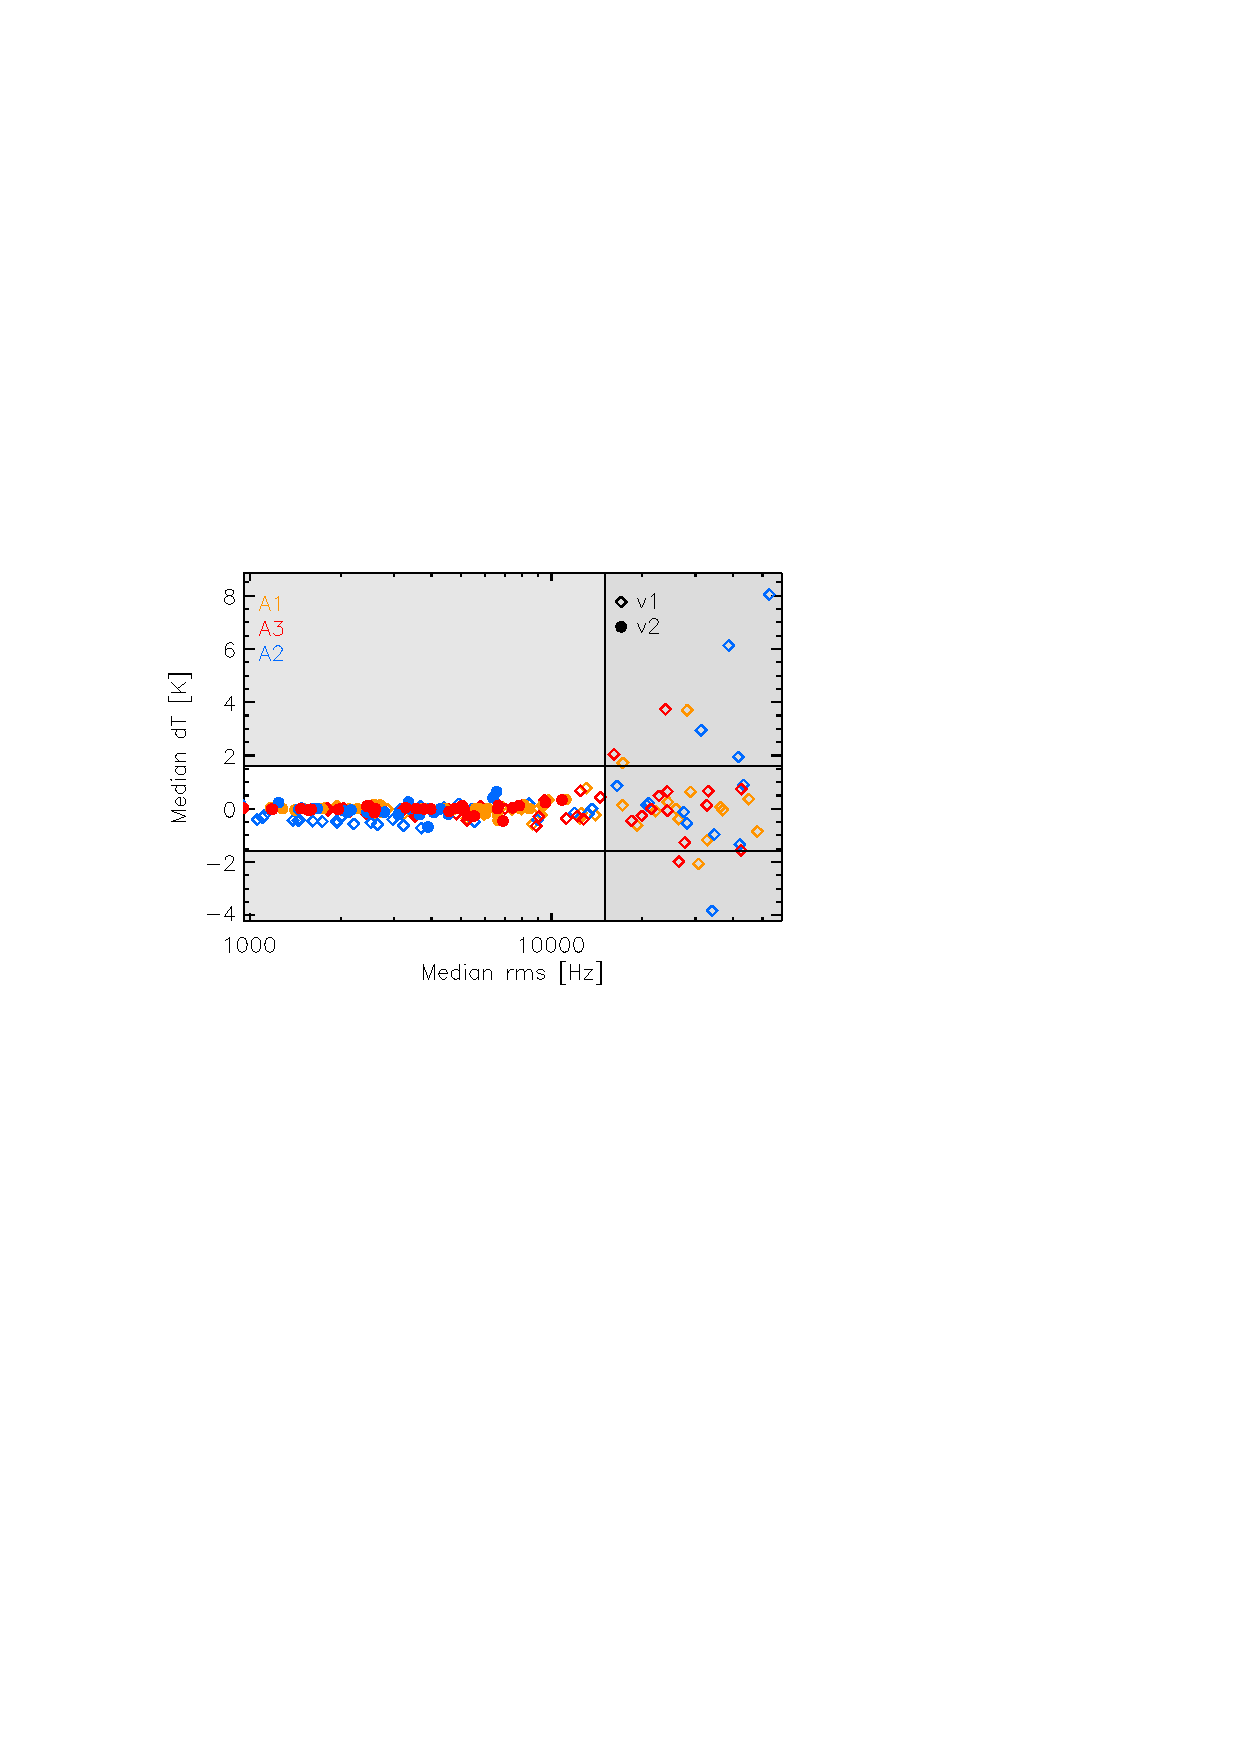
\includegraphics[clip=true,width=0.9\linewidth]{Figures/Opacity/plot_skydip_selection_two_crit.pdf}
\caption[N2R9 skydip scan selection.]{ Median dT quality-fit criterion is plotted in fonction of Median rms criterion for each skydip scans of the N2R9 campaign and for the three arrays. Both criteria are nicely correlated. Empty diamonds show the results of the first iteration of the skydip coefficient estimation, whereas filled circled show the second iteration, for which only the skydips that met both fit-quality criteria are included. After the second iteration, all the remaining skydips met the criteria.}
\label{fig:skydipselection}
\end{center}
\end{figure}

For each skydip scan and for each bunch of 40 KIDs, we compute the
difference between the measured KID resonance frequency and the model
given in Eq.~\ref{eq:skydip} taken at the best-fit values of the
($C_0$, $C_1$) parameters. Then we determine two indicators
of the fit quality per skydip. First, the standard deviation of the
measure-to-model difference is calculated over all the KIDs in a
bunch. For each skydip, we evaluate the median rms, which is the
median over the KID bunches of the standard deviation per bunch, given
in Hz. Secondly, for each scan, we compute the average
measure-to-model difference of each KID $k$, labelled $dT_k$, which is
then converted from Hertz to Kelvin using the $C_1$ parameter of the
KID $k$. Median $dT$ is the median of $dT_k$ over all the KID of an
array. With these two indicators in hands, we discard the skydip scans
that are noisy or that yield a poor fit by applying the selection
criteria

\begin{itemize}
\item Median $\rm{rms} < 1.5 \times 10^{4}~\rm{Hz}$
\item Median $dT < 1.6~\rm{K}$
\end{itemize}

The threshold values have been determined using the set of 44 skydip
scans of N2R9. The Median rms cut corresponds to twice the median of
this quantity per skydip scan, whereas the Median $dT$ cut is twice
the standard deviation of Median $dT$ over the skydips. N2R9 skydip
scan selection is illustrated in Fig.~\ref{fig:skydipselection}, in
which the agreement between the two fit-quality criteria is clearly
seen. The ($C_0$, $C_1$) estimation proceeds in two steps: first the
parameters are estimated using all the available skydip scan for a
given campaign, then the estimation is re-iterated using the only
skydip scans that met the fit-quality criteria. After the second
iteration, we check that no extra skydip outlier are left, as shown by
the 'v2' label data points in Fig.~\ref{fig:skydipselection}.


\addparag{stability against the skydip scan selection + FIG}
We test the stability of the ($C_0$, $C_1$) parameters against the exact choice of the selection criteria.  
At 1mm, we find about {\color{red} $[$TBC$]$  $10\%$} opacity variation from very inclusive to very aggressive selections. However, at 2mm, this scatter reachs about {\color{red} $[$TBC$]$  $30\%$} relative uncertainties.


We conclude that opacities at 1mm can be reliably estimated from a series of skydip scans using the (C0, C1) model. By contrast, for the 2mm opacities, a skydip-based method is not stable enough against the skydip selection. Thus, we adopt an hybrid approach. 

%\section{The hybrid method}

%The hybrid method comprizes two-steps: i) first the 1mm opacities,
%that are $\tau_{A1}$ and $\tau_{A3}$, are determined using the skydip
%method described in Sect.~\ref{se:skydip-method}, ii) then the 2mm
%opacity $\tau_{A2}$ is extrapolated from the 1mm ones using a modified
%ATM model. Namely, for the second step, we perform:

%\begin{equation}
%\tau_{A2} = \left( \left.\frac{\tau_{A2}^{\rm{ATM}}}{\tau_{A3}^{\rm{ATM}}}\right\vert_{\tau_{A3}} + \alpha \right) \tau_{A3},
%\end{equation}

% where $\alpha$ is an offset, which are estimated from the observations themselves, and the ratio is the predicted zenith opacity ratio for A2 and A3 frequency bands using the ATM model described in \ref{Pardo2002} and taken at the measured A3 zenith opacity. The zenith opacity expectations for the array $A_i$ is
%\begin{equation}
%  \tau^{\rm{ATM}}_{A_i} = - \ln{\frac{\int e^{-\tau^{ATM}(\nu)} T_{A_i}(\nu) d\nu}{ \int T_{A_i}(\nu) d\nu}},
%\end{equation}
%where the bandpasses $T_{A_i}$ for arrays $A_i$, $i=1, 2, 3$, are the Martin-Pupplet reference transmissions
%corrected by a Rayleigh-Jeans term  $T'_{A_i}(\nu) / \left( \frac{\nu}{\nu_0}\right)^2$. 

%We observe that the measured \emph{shape} of the measured opacity ratio is well described by the ATM expectations whereas its \emph{amplitude} is too low by an offset $\alpha$, which we dertermine using a data-driven approach. We estimate $\alpha$ as the offset that ensures a stability of the A2 flux over the whole opacity span.  

%\addparag{$\alpha$ fit + FIG}



%----------------------------------------------------------------------------------------
%	Corrected skydip method
%----------------------------------------------------------------------------------------
\section{Corrected skydip method}
\label{se:corrected-skydip}




%----------------------------------------------------------------------------------------
%	Tests
%----------------------------------------------------------------------------------------
\section{Opacity measurements}
\label{se:opacity_correction}

%{\bf copy from the 'Instru' paper}

%\begin{figure}[ht]
%\begin{center}
%\includegraphics[scale=0.8]{Figures/test_allskd_N2R10v3commiss2.pdf}
%\caption{Atmospheric opacity as measured from the NIKA2 data 
%at 260 (top) and 150\,GHz (bottom) during N2R10
%commissioning campaign. Each block of 40 KIDs gives an independent estimate of
%the opacity value for each skydip scan (the integer abscissae). The block
%number is the decimal value of the abscissae.
%\label{fig:taumeas_paper}}
%\end{center}
%\end{figure}

%\begin{figure}[ht]
%\begin{center}
%\includegraphics[scale=0.8]{Figures/test_allskd_N2R10v2commiss1.pdf}
%\caption{Atmospheric opacity as measured from the NIKA2 data 
%at 260 and 150\,GHz during N2R10
%commissioning campaign. The error bars are in fact dispersion of the deduced
%opacities between blocks of 40 KIDs.
%\label{fig:taumeas_paper}}
%\end{center}
%\end{figure}

We observe that the skydip-fitted $\tau$ values are, as expected, common
between different detectors of the same array. By comparing the results of different skydips, we
have verified experimentally that the coefficients $C_0$, $C_1$ are stable,
within the fit errors, on very long time scales within a cooldown cycle. The
coefficients can thus be applied to the whole observing campaign in order to
recover the opacity of each scan.


% \noindent {\bf FM : a figure would help to convince the reader that it is stable on lng time
% scale, which is a key point.}\\ FXD: I will do that figure


\begin{figure}[ht]
\begin{center}
\includegraphics[scale=0.8]{../../../Paper_NIKA2_Technical/opacity_evol_run22.pdf}
\caption[Zenith opacity monitoring during N2R9]{Atmospheric opacity as measured from the IRAM 225\,GHz taumeter
(cyan), and from the NIKA2 data at 150 (red) and 260\,GHz (blue) during N2R9
commissioning campaign (Feb. 2017). We stress the fact that the IRAM 225\,GHz
taumeter data is not used for the atmospheric correction and is plotted here
just for comparison.
  \label{fig:taumeas_paper}}
\end{center}
\end{figure}


\begin{figure}[ht]
\begin{center}
\includegraphics[width=\linewidth]{Figures/opacity_vs_index_N2R9_N2R10.png}
\caption[Zenith opacity monitoring during N2R9 and N2R10]{Atmospheric opacity as measured from the IRAM 225\,GHz
  taumeter (black crosses), and from the NIKA2 data at 150 (red) and 260\,GHz (blue) during 
  N2R9 and N2R10 commissioning campaigns.  We stress the fact that the IRAM 225\,GHz taumeter data is not used for the atmospheric correction and is plotted here just for comparison.
  \label{fig:taumeas}}
\end{center}
\end{figure}


In Fig.~\ref{fig:taumeas} {\bf(and Fig.~\ref{fig:taumeas_paper} of
  \cite{Adam18}) } we present the evolution of the NIKA2 in-band
opacities for all the 'OTF' scans (about 1300 scans per runs) of the
N2R9 run held in February and the N2R10 run in April 2017. These are
compared to the IRAM tau-meter values. We observe an agreement on the global trend between the IRAM tau-meter opacity (225 GHz) and the NIKA2 values. These latter show, however,
a smaller dispersion (less than one percent).





\clearpage
%----------------------------------------------------------------------------------------
%	FOCAL PLANE RECONSTRUCTION
%----------------------------------------------------------------------------------------
\section{Focal Plane Reconstruction}
\label{se:fp_reconstruction}
%----------------------------------------------------------------------------------------
%	FOCAL PLANE RECONSTRUCTION
%----------------------------------------------------------------------------------------
%\section{Focal Plane Geometry}
%\label{se:geometry}


%   Methods
%----------------------------------------------------------------------------------------
\subsection{FOV position reconstruction}
\label{se:fov_geometry}

In order to be able to produce a map, one needs to associate a pointing
direction to any data sample of the system. The telescope provides us with
various pointing information for a reference position in the focal plane. We
then need to know the relative pointing offsets of each detector. We use
\bms\ for this purpose (see Sect.~\ref{se:beammaps}). The determination of the
KID offsets in the focal plane proceeds in two steps.

\paragraph{Step 1.} We apply a median filter per
KID timeline whose width is of 31 samples, that is equivalent to about 
5~FWHM at 65 arcsec/s given that the sampling frequency is 23.84~Hz,
and we project one map per KID in Nasmyth
coordinates. This median filter removes
efficiently most of the low frequency atmospheric and electronic
noise, albeit with a slight ringing and flux loss on the
source. However, at this stage, we are only interested in the location
of the observed planet.
To derive the Nasmyth coordinates from the
provided $(\alpha_t,\delta_t)$ and $(\Delta\alpha_t,\Delta\delta_t)$
coordinates, we build the following quantities at time~$t$:

\begin{eqnarray}
\Delta x_t &=& \cos\delta_t \Delta\alpha_t - \sin \delta_t\Delta \delta_t \nonumber \\
\Delta y_t &=& \sin\delta_t \Delta\alpha_t + \cos \delta_t\Delta \delta_t \nonumber
\end{eqnarray}

Note that $\Delta\alpha_t$ is already corrected by the $\cos\delta_t$ factor to
have orthonormal coordinates in the tangent plane of the sky and be immune to
the geodesic convergence at the poles. Moreover, before projecting the
time-ordered data onto maps, we check
the accuracy of the time-stamping and the consistency between the
telescope time and NIKA2 time. First, we test the
synchronisation of the electronic boxes and the regularity of the
time increase. In case of detection of an anomaly, the
time-stamping of the impacted data samples is
recalculated by interpolating from the accurately stamped
neighbour samples. Then, a so-called \emph{zigzag}
procedure is used to test for delay between the telescope pointing
information and NIKA2 timelines: we fit a constant shift between the
source positions estimated using the subscans in one direction and
using the subscans in the opposite direction. The data timelines are
then projected onto maps. 
We fit a 2D elliptical Gaussian on
each KID map. The centroid of this Gaussian is a first estimate of the KID
offsets, FWHM's, ellipticity and sensitivity. We apply a first KID selection by
removing outliers to the statistics on these parameters. We also discard
manually KIDs that show a cross-talk counterpart on their map.

\paragraph{Step 2.} With these offsets, it is already possible to produce maps
from the combination of all detectors. However, in order to go up to
the calibration stage, we must correct for the flux loss induced by
the median filter and ensure that each timeline is treated in the same
way as the final observation will. For this, we apply the pointing
reconstruction presented in Sect.~\ref{se:ptg} and the data reduction
presented in Sect.~\ref{se:toi_proc}. We still do not have absolute
calibration for each KID (no opacity correction yet) but the amplitude
of the fitted centroid on the same planet provides the required
cross-calibration between KIDs. The final absolute calibration will be
presented in Sect.~\ref{se:calibration}.\\

This analysis is repeated on all \bms\ to obtain statistics and
precision on each KID parameter, together with estimates on KID
performance stability, as discussed in the next sections.

\subsection{FOV grid distortion}
\label{se:grid_distortion}

We studied the matching of the KID position on the sky to the
design position. The global result is scaling, rotation, and shift
parameters for each array. They are described in Table~\ref{ta:gridmatch}.

\begin{table}[ht]
\label{ta:gridmatch}
\begin{center}
\begin{tabular}{|c|c|c|l|}
\hline
Array 1  &	Array 3   &	Array 2   &	Comment \\
\hline
1.25     &      1.25      &     2.05     &     \small{$\lambda$ in mm} \\
1140 	 &      1140 	   &        616  &     \small{Total of designed KIDs (TDK)} \\
673/736  &	734/758  &	437/444  &     \small{Well-placed KIDs (WPK)/Found KIDs (FK)} \\
91/59 	 &    96/64 	 &      98/71 	 & \small{Ratio [\%] of WPK/FK and WPK/TDK} \\
0.87 	 &     0.84 	  & 0.66     &	\small{Median deviation [arcsec] for detectors deviating by less than 5~arcsec} \\
0.52 	 &     0.69 	 &        0.68 	 & \small{Mean distortion across the FoV in arcsec} \\
2.3 -4.5  &	2.0 -5.8  &	9.3 -7.5  &	\small{Array center in Nasmyth coordinates [arcsec]} \\
4.90  &	4.88  &	4.88  &	\small{Plate scaling [arcsec/mm] in the Design x and y (averaged)} \\
77.3  &	76.4  &	78.2  &	\small{Plate rotation angle [degree] from the Design to Nasmyth coordinates} \\
6.6  &	6.6  &	6.6  &	\small{FOV [arcmin] (Total KIDs)} \\
9.8/2.00  &	9.7/2.00  &	13.3/2.75  &	\small{Distance between near detectors [arcsec, mm]} \\
% Old values, rechecked (difference comes from lambda and D)
%   1.24  &	1.22  &	0.97  &	Distance between near detectors with $30\,\rm{m}$ diameter aperture [in $\lambda$/D] \\
% here new values checked FXD 30 Nov 2018:
1.11  &	1.10  &	0.87  &	\small{Measured Distance between near
  detectors [in $\lambda$/D] } \\
%\new{with $27\,\rm{m}$ effective diameter aperture} [in $\lambda$/D]} \\
1.09  & 1.09  & 0.93  & \small{Modeled Distance with ZEMAX}\\
\hline
\end{tabular}
\end{center}
\caption[Field-of-view deformations]{Linear 2D fit of the observed
  position of the detectors in the sky for N2R9 against their mechanically
  designed position. The initial table of Found KIDs is given
  by the focal plane geometry procedure, as described in
  Sect.~\ref{se:fov_geometry},
  applied to N2R9 \bm\ scans. More than 90\% of the detectors (WPK/FK) are
  within less than 5 arcseconds of their expected position. }
\end{table}

It shows that on average the position of each detector is known to better than
an arcsecond. The 1\,mm arrays have almost the same center but this center
differs by 7 and 2\,arcsec in Nasmyth coordinates from the
2\,mm array center. The sampling is above
$\lambda/D$ at 1\,mm, assuming a 27\,m effective diameter aperture. Note that
the plate rotation angle was designed as 76.2\,degrees, less than 2
degrees from what is observed. We find that array 1
has some of the most deviant detectors (above 4\,arcsec from their expected
position). These detectors should be excluded from further analysis. We call
distortion (in the table) the $x.y$ term in the polynomial fitting between the
design grid and the observed position (the fitting is done with the $x$ and
$y$ linear terms and the $x.y$ term). 

This has been compared to expectations obtained using ZEMAX
simulation. 
%The grid diagram generated using ZEMAX provides us with
%the maximum dispersion in the field defined by
%
%\begin{equation}
%P = \frac{\sqrt{(x_p - x_r)^2 + (y_p - y_r)^2}}{\sqrt{x_p^2 + y_p^2}},
%\end{equation}
%
%where $(x_p, y_p)$ and $(x_r, y_r)$ are respectivelly the predicted
%and real coordinates on the image surface relative to the reference
%field position image location (see page 170 of the ZEMAX manual, 2007).
%The predicted coordinates for the whole field are obtained using a
%linear interpolation of a small area in the field central part,
%whereas the real coordinates are calculated by ray tracing through the
%optical system.
%
%\begin{figure}[ht] 
%\begin{center}
%  \includegraphics[width=0.9\textwidth]{Figures/NIKA2_Grid-distortion.png}
%  \caption[Simulated FOV grid]{NIKA2 grid diagram simulated using
%    ZEMAX. \new{The step of the grid is of 30 arcsec and the side width
%      of the black square is of seven arcmin. The red circle corresponds to the 
%      $6.5\,\rm{arcmin}$ diameter FOV. Blue crosses show the grid
%      distorsions in az-el coordinates and in the case of an observing
%      elevation of $14^o$. These grid distorsions depends on the
%      telescope elevation, whereas in the image plane (the plane of the
%      KID arrays) the distorsions are invariant. This allows for
%      concluding that the grid distorsions are caused by the optical
%      elements located between M4 and the dichroic plate.} 
%  }
% \label{fig:fov_grid_distortion_zemax}
%\end{center}
%\end{figure}
%Figure \ref{fig:fov_grid_distortion_zemax} shows the ZEMAX grid diagram for
%NIKA2 simulated optic system.
%
We generated a grid diagram for NIKA2 optic system and found a maximum
grid distortion of $2.7\%$ in the $6.5'$ FOV. We notice that the
strongest distortion appear in the upper right corner of the Nasmyth plan, which is
also the area of the largest defocus w.r.t. to the center (see
Sect.~\ref{sec:focus_surfaces}).
An expected distortion of $2.7\%$ is at most a 5'' shift from the
center to the outside of the array. The quoted distortions between the
measured and designed positions are consistent with the expected
maximum distortions from the NIKA2 optics.

%Auxillary information on this work can be found in this wiki post\footnote{\tiny
%  {\tt http$://$www.iram.fr$/$wiki$/$nika2$/$index.php$/$April$\_$19,$\_$2017,$\_$FXD,$\_$KID$\_$position$\_$mapping$\_$and$\_$Field$\_$distortion$\_$for$\_$Run9}}.
% FXD: this would need to be more ascertained. Lack of time to go further.


\subsection{KID selection and average geometry}
\label{avg_kidpar}

\begin{figure*}[!tp]
\begin{center}
\includegraphics[trim=2cm 14cm 4cm 4cm, clip=true,width=0.45\linewidth]{Figures/A1_fwhm_color_count.pdf}
%\includegraphics[trim=2cm 14cm 5cm 4cm, clip=true,width=0.45\linewidth]{Figures/A1_positions.pdf}
\includegraphics[trim=2cm 14cm 4cm 4cm, clip=true,width=0.45\linewidth]{Figures/A3_fwhm_color_count.pdf}
%\includegraphics[trim=2cm 14cm 5cm 4cm, clip=true,width=0.45\linewidth]{Figures/A3_positions.pdf}
\includegraphics[trim=2cm 14cm 4cm 4cm, clip=true,width=0.45\linewidth]{Figures/A2_fwhm_color_count.pdf}
%\includegraphics[trim=2cm 14cm 5cm 4cm, clip=true,width=0.45\linewidth]{Figures/A2_positions.pdf}
\caption[KID selection in the FOV]{Average detector positions
  for arrays A1, A3, and A2. The three plots show the detectors that have seen
  the sky and passed the quality criteria for at least two \bms\ during Run10, 9
  and 8: 952, 961, and 553 for A1, A3 and A2, respectively. The color
  indicates, from green to red, how many times a KID was
  identified as valid on a \bm. The inner and outer
  dash-line circles correspond to a FOV of 5.5\,arcmin and 6.5\,arcmin,
  respectively. Units are arcseconds.}
\label{fig:avg_fov_color}
\end{center}
\end{figure}

In order to identify the most stable KIDs, we compare the KID parameters
obtained with several \bms.  In the following, we show results as obtained using
seven \bms\ from Run10, two from Run9 and one from Run8.  For each KID we
compute the average position on the focal plane and the average FWHM, counting
the times that it has been considered as valid and at the same position. Indeed,
a few KIDs have close resonances and can be tuned and switched on some scans. A
few others must also be discarded because they appear identical numerically due
to \samu{the fact that a same (noisy) KID can sometimes be associated
  to two different frequency tone in the acquisition.}
%a remaining artefact in the acquisition.
These KIDs are flagged out (less than 1\% of the designed KIDs).

In Fig.~\ref{fig:avg_fov_color} we show the
average focal plane reconstruction, from green to red depending on the number of
times that the KID has been considered as valid.
\new{The eight internal readout feed lines that connect each of the two
  $1\,\rm{mm}$ arrays are also noticeable in this figure: first, slightly
  larger spaces are seen between KID rows connected to different
  feed-lines than between KID rows of the same feed line and second, KIDs at the end of a
  feed line are less often valid than others (see e.g. the FOV of
  Array 3). For A1, this end-of-feedline effect is mixed with the
  effect of the KID gain variation across the FOV, which mainly affects
  the South-West third of the array, as discussed in Sect.~\ref{se:flatfields}.}

For A1, A3 and A2, respectively, we have 952, 961, and 553 KIDs that
have been considered as valid at least twice (840, 508, 868 valid at
least five times). Using this criterion, we deduce the fraction of
valid detectors over the designed ones, as given in Table~\ref{tab:number_of_kids}.

%% \begin{figure}[htp]
%% \begin{center}
%% \includegraphics[trim=2cm 14cm 5cm 4cm, clip=true,width=0.55\linewidth]{Figures/A1_positions.pdf}
%% \includegraphics[trim=2cm 14cm 5cm 4cm, clip=true,width=0.55\linewidth]{Figures/A3_positions.pdf}
%% \includegraphics[trim=2cm 14cm 5cm 4cm, clip=true,width=0.55\linewidth]{Figures/A2_positions.pdf}
%% \caption[Stability of KID positions in the field-of-view]{For the valid
%%   detectors, we show the positions of each pixel, as obtained from each beam
%%   map. Some of them are not found at the same position for all the \bms.
%% Units are arcseconds. \todo{{\bf FM : color code : same as on the 1st
%%       maps of validity}}}
%% \label{fig:jumping_kids}
%% \end{center}
%% \end{figure}

%\begin{figure}[htp]
%\begin{center}
%\includegraphics[trim=2cm 14cm 5cm 4cm, clip=true,width=0.55\linewidth]{Figures/A1_test_positions.pdf}
%\includegraphics[trim=2cm 14cm 5cm 4cm, clip=true,width=0.55\linewidth]{Figures/A3_test_positions.pdf}
%\includegraphics[trim=2cm 14cm 5cm 4cm, clip=true,width=0.55\linewidth]{Figures/A2_test_positions.pdf}
%\caption[Average KID positions]{For the valid detectors,
%  we show the mean (red crosses) and the median (black squares)
%  positions of each pixel, as obtained from each \bm.
%  Units are arcseconds. \todo{FM : color code ? same as on the 1st maps of validity}}
%\label{fig:mean_vs_median}
%\end{center}
%\end{figure}

\begin{table}[ht]
\begin{center}  
  \begin{tabular}{|c|c|c|c|}
    \hline
    Array & Designed detectors &  Valid detectors & Fraction\\
    \hline\hline
    A1 & 1140 & 952 &  84\%\\
    A3 & 1140 & 961 &  84\%\\
    A2 & 616  & 553 &  90\%\\
    \hline
  \end{tabular}
  \caption[Number of detectors]{Summary of the number of valid detectors per array.}
  \label{tab:number_of_kids}
\end{center}    
\end{table}


% + Focal Plane Geometry
% + KID selection and average geometry
% + FOV grid distortion
% + Reconstruction of the focus surfaces


\clearpage
%----------------------------------------------------------------------------------------
%	BEAM PATTERN
%----------------------------------------------------------------------------------------
\section{Beam pattern}
\label{se:beams}
%%
%%
%%      SECTION: BEAM PATTERN 
%%

%% [intro]
%%________________________________________________________

The NIKA2 beam pattern mainly depends on the IRAM 30m telescope and
NIKA2 full (external and internal) optical system characteristics,
whereas the detectors themselve might have an impact at sub-dominant
level (through e.g. time constants or correlated noises). In this
section, first we reconstruct the focus surfaces and present the
optimal focus, then we characterize both the main beam, which is
modeled as an elliptical Gaussian, and the full beam pattern including
error beams up to angular scales of 10 arcmin.



%% [Optimal Focus]
%%________________________________________________________
\subsection{Optimal focus}
\label{sec:focus}

Owing to the NIKA2 $6.5~\rm{arcmin}$ FOV, the focus is expected to
slightly changes across the FOV, defining curved focal surfaces at the
location of the three arrays. Therefore, beam patterns are expected to
show some scatter across the FOV accordingly to the focal
surfaces. Although all the detectors cannot be individually focalised,
an optimal axial focus of the telescope can be found to maximize the
number of detectors at the best focus and hence, maximize the
resolution of the NIKA2 maps. This optimal z-focus setting is obtained
in measuring the focus at the center of the arrays as described
Sect.~\ref{sec:focus-meas} and apply a focus shift, which is primary
predicted using Zemax simulation, and ultimately verified by measuring
the focus surfaces, as decribed in Sect.~\ref{sec:focus-surf}.


\subsubsection{Focus estimation}
\label{sec:focus-meas}

The best axial focus in the central region of the arrays is estimated
using the so-called 'focus$\_$OTF' PAKO script, which realises a
series of five $1' \times 5'$ OTF scans at various values of
the focus in $0.4~\rm{mm}$-steps around an \emph{a priori} value $z_0$,
namely $z \in \{-0.8, -0.4, 0, 0.4, 0.8\} + z_0$. Elliptical Gaussian
fits on the reconstructed maps provide estimates of the flux and FWHM
along minor- and major-axis for each focus. Then, parabolic fits are
used to determine the best focus. We consider three estimates: i)
$\hat z_{\rm{peak}}$ the focus that maximizes the estimated flux,
which is the amplitude of the 2D Gaussian, 
ii) $\hat z_{\rm{fwhm}}$ the focus that
minimizes the geometrical FWHM, defined as the quadratic mean of
$\rm{FWHM}_{\rm{major}}$ and $\rm{FWHM}_{\rm{minor}}$,  and iii)
$\hat z_{\rm{ellipt}}$ the focus that minimizes the beam ellipticity,
defined as $\rm{FWHM}_{\rm{major}}/\rm{FWHM}_{\rm{minor}}$.
Fig.~\ref{fig:focus-example} shows an example of
axial focus measurement using a 'focus$\_$OTF' observation of Neptune
during N2R10.

\begin{figure}
\begin{center}
  \includegraphics[clip, angle=0, scale=0.25]{Figures/plot_20170419s143.png}
\caption{Example of axial focus measurment using a 'focus$\_$OTF' observation of Neptune
during N2R10 [PLACEHOLDER]}
\label{fig:focus-example}
\end{center}
\end{figure}


\subsubsection{Focus consistency between arrays}

{\bf refaire les plots de difference de focus entre matrices }

\subsubsection{Reconstruction of the focus surfaces}
\label{sec:focus-surf}

\begin{figure}
\begin{center}
  \includegraphics[trim={0, 1cm, 0, 1cm}, clip, angle=0, scale=0.5]{Figures/fov_focus_mv_5.png}
\caption{Focus surface of A1, A3 and A2 arrays from left to
  right. From top to bottom, the focus estimates rely on
  FWHM-minimization, amplitude-maximization of an elliptical
  Gaussian of fixed FWHMs and amplitude-maximization of an elliptical
  Gaussian.}
\label{fig:focus-surfaces}
\end{center}
\end{figure}

\emph{Method. } We measure NIKA2 focal surfaces by means of a sequence of five 'beam-map'
scan observations of bright point-like sources, typically Planets or
bright quasars,
for various settings of the telescope axial focus around the
optimal focus $z_{\rm{opt}}$. A beam-map scan consists of a deep-integrated
$13.5' \times 7.8'$ OTF-scan observation comprizing $99$ sub-scans and
with a scanning speed of either $65''/s$ whenever the mean integration
elevation is $< 60$ degree or $39"/s$ at higher elevation. The z-focus is changed in step of
$0.6~\rm{mm}$ to probe a large focus range for measuring even the
extreme variation of the focus surfaces,
namely $z \in \{-1.2, -0.6, 0, 0.6, 1.2 \} + z_{\rm{opt}}$.
Each beam-map scans allow for $4''$-resolution individual maps per kid to
be projected. Before the projection, the correlated noise is mitigated
from each KID timeline in subtrating out a common mode, which is obtained
using, amongst the other detectors, those that correlates the most
with this KID and that are located outside a radius of $90''$
around the source centroid.
Therefore, a series of five cleaned maps at various focus is
available for each detector, from which the best focus is estimated as
described in Sect.~\ref{sec:focus-meas}. The ensemble of the relative
focus estimate per KIDs with respect to the best focus at the center
of the array constitutes the focus surface. An accurate estimate of
the center focus is obtained as the
weighted average focus estimate of the KIDs lying in a $30''$ radius
around the geometrical center of the array. This average does not
induce any sizeable bias thanks to the flatness of the focus surface
in the innermost regions. For robustness test, we consider three focus
estimates: the two first ones are the same as discussed in
Sect.~\ref{sec:focus-meas} -- namely i) $\hat z_{\rm{fwhm}}$ the focus that
minimizes the geometrical FWHM and ii) $\hat z_{\rm{peak}}$ the focus
that maximizes the amplitude of the best-fitting ellitical Gaussian --
whereas the third one is $\hat z_{\rm{flux}}$ the focus that maximizes
the amplitude of the best-fitting elliptical Gaussian of fixed FWHM
(at $12''$ at $260~\rm{GHz}$ and $18''$ at $150~\rm{GHz}$). The 
comparison between the two amplitude-based estimators
($\hat z_{\rm{peak}}$ and $\hat z_{\rm{flux}}$), will test the
stability of the focus results against the exact choice of the beam fitting
function. Since the ellipticity-based estimator $\hat z_{\rm{ellip}}$ is
less sensitive to focus changes and yields larger uncertainties than the
others, we do not use it for the focus surface reconstruction.     


\emph{Data selection. }
During the three commissioning campaigns that occured after the change of A1
lens and the improvement of internal optics alignment (hence in the
final NIKA2 optic configuration),
nine out-of-focus
beam-map scan sequences have been acquired, including incomplete
sequences and sequences hindered by poor atmospheric conditions. We
select sequences that i) comprises at least four scans, ii) have been
observed at zenith opacity at $225~\rm{GHz}$ (as indicated by
the IRAM taumeter) below 0.5 and iii) have a maximal central focus
drift between the starting time and the end of the sequence of
$0.5~\rm{mm}$. These criteria preserve five sequences from which focus
surfaces can be reconstructed. Namely, we consider the sequences
$20170226s415\mbox{--}419$, $20170419s133\mbox{--}137$, $20170420s113\mbox{--}117$,
$20170421s160\mbox{--}164$ and $20170424s123\mbox{--}127$, which consist of observations
of the bright quasar '3C84' and Neptune.

\emph{Results. }
For each detector $k$ and each beam-map sequence $s$, we obtain for
the array $a$, a focus measurement $z_k^{a, s} \pm \sigma_k^{a, s}$,
where $\sigma_k^{a, s}$ is the $1\mbox{--}\sigma$ error of the least-square
polynomial fit. The focus surface measurements per array obtained from the five
beam-map sequences are combined using an inverse-variance weighting
scheme to obtain the focus surface estimates 
\begin{equation}
\label{eq:mv_focus_surf}
z_k^{(a)} = \left( \sigma_k^{(a)} \right)^2 \,  \sum_s \frac{z_k^{a,s}}{\left(\sigma_k^{a,s}\right)^2}\, \,  ,
\end{equation}
with uncertainties 
\begin{equation}
\label{eq:error_mv_focus_surf}
\sigma_k^{(a)} = \left[ \sum_s \frac{1}{\left(\sigma_k^{a,s}\right)^2}\right]^{-1/2}\, .
\end{equation}


We present NIKA2 focus surfaces per arrays obtained as in
Eq.~\ref{eq:mv_focus_surf} 
%from the inverse-variance weighted combination of the five
%reconstructed focus surfaces per arrays
in Fig.~\ref{fig:focus-surfaces}.
The three flavours of focus-estimators provide us with focus surfaces
per arrays that are in good agreement with each others and that have a
non-axisymetrical flatten bowl shape consistent with expectations from
simulation {\bf [TBA, as discussed further below]}.
The median defocus (that is the relative focus w.r.t. the center)
across the detectors is about
$-0.1~\rm{mm}$ for the three arrays. Maximal defocus values of about
$-0.6~\rm{mm}$ are found for detectors located in the outer top and
left regions of the FOV. Finally, a fraction comprised between $20$
and $30\%$ of the KIDs has a relative $z\le -0.2~\rm{mm}$.  

We primarily estimate the uncertainty of the focus
surface measurements using the standard deviation between the three
estimators $z_k^{(a)}|_{\rm{fwhm}}$, $z_k^{(a)}|_{\rm{peak}}$ and
$z_k^{(a)}|_{\rm{flux}}$. We found approximatively homogeneous
standard deviation surfaces per arrays, which have median values across
the FOV of about $0.03~\rm{mm}$.
However, we cross-check this error estimate by forming the quadratic mean of
the three inverse-variance error surfaces per arrays, which are defined in
Eq.~\ref{eq:error_mv_focus_surf} and quoted
$\sigma_k^{(a)}|_{\rm{fwhm}}$, $\sigma_k^{(a)}|_{\rm{peak}}$ and
$\sigma_k^{(a)}|_{\rm{flux}}$. This provides us with more optimistic
error surfaces per array, which do not show any clear pattern across
the FOV and which have a median value across the detectors of about
$0.015~\rm{mm}$.  

%[EXPAND THE DISCUSSION ON COMPARISON WITH SIMULATION]

\emph{Stability across sequences. }
By comparing the focus surface obtained from the five individual focus
sequences, we test the stability of the NIKA2 focus surfaces across
the time and the atmospheric conditions. In
Figs.~\ref{fig:focus-stability-H}-\ref{fig:focus-stability-V}, we compare
the defocus along two perpendicular diameters across the
FOV. Although any direction would have been equivalent for this test, we choose to
position the diameters along-with and perpendicular-to the KID geometrical
grid to avoid the scatter due to KID non-alignement in any other
direction. The scatter is further mitigated by considering
four-detector-wide diameters as shown in upper the left corner of
Figs.~\ref{fig:focus-stability-H}-\ref{fig:focus-stability-V}.

{\bf add a sentence to conclude on the stability}


\begin{figure}
  %\begin{center}
  \includegraphics[trim={-2cm, 2cm, 0, 2cm}, clip, angle=0, scale=0.1]{Figures/fov_focus_stability_check_D1.png}
  \begin{center}
  \includegraphics[trim={0, 2cm, 0, 2cm}, clip, angle=0, scale=0.45]{Figures/fov_focus_1D_Vband_5.png}
  \end{center}
  \caption{Stability of the focus surface across the sequences. This
    series of plot show the relative focus with respect to the center
    (defocus) along the 'vertical diameter', that is a band of
    four-detector width across the FOV, which is vertical with respect to
    the detector geometrical grid, as illustrated by the plot in the
    upper left corner. The datapoints show the defocus along the
    'vertical diameter' estimated from the five focus sequences,
    namely $20170226s415\mbox{--}419$ (sky blue),
    $20170419s133\mbox{--}137$ (dark blue), $20170420s113\mbox{--}117$ (red),
    $20170421s160\mbox{--}164$ (yellow) and $20170424s123\mbox{--}127$
    (green), using the $z^{(a)}|_{\rm{fwhm}}$, $z^{(a)}|_{\rm{flux}}$ and
    $z^{(a)}|_{\rm{peak}}$ estimators from top to bottom, and for A1, A3 and
    A2 arrays from left to right. The black datapoints are the five-sequence combined defocus, as
    presented in Fig.~\ref{fig:focus-surfaces}, taken along the
    'vertical diameter', and the errorbars, the
    five-sequence combined defocus errors along the 'vertical
    diameter'.}
\label{fig:focus-stability-H}
\end{figure}


\begin{figure}  
  \begin{center}
  \includegraphics[trim={0, 2cm, 0, 2cm},clip, angle=0, scale=0.45]{Figures/fov_focus_1D_Hband_5.png}
  \caption{Stability of the focus surface across the sequences. Same
    legend as in Fig.~\ref{fig:focus-stability-H}, but for the
    detectors located in an 'horizontal diameter', i.e. a band of
    four-detector width across the FOV, which is horizontal with respect to
    the detector geometrical grid, as illustrated by the plot in the
    upper left corner. }
\label{fig:focus-stability-V}
\end{center}
\end{figure}


\subsubsection{Constraints on the X and Y foci}
\label{sec:focus_X_Y}

{\bf add a description of the method}

{\bf expand a little the discussion below}

Very delicate measurements

The plan is to devote a few hours of technical observation time in
good weather condition to perform an accurate measure of NIKA2 lateral
focus. The X-, Y-focus will then be set at these robust estimated vallues and
checked only a few times a year (at the seasonal change for example).  


Figures \ref{fig:X_focus} and \ref{fig:Y_focus} show examples of the
lateral focus measurements performed during \emph{N2R9}. 

\begin{figure*}[h!]
\centering
\includegraphics[height=8cm]{Figures/plot_20170223s39.png}
\hspace{0.5cm}
\includegraphics[height=8cm]{Figures/residuals_focus_otf_20170223s39.png}
\caption{{\footnotesize \textbf{Left:} X-focus measurement using a
    parabolic fit of the flux, beam fwhm and ellipticity on a sequence
    of five OTF scans on Uranus (20170223s39-43) \textbf{Right:} Beam residuals after subtracting a model of the main beam for each OTF-scan of the X-focus session.}}
\label{fig:X_focus}
\end{figure*}

\begin{figure*}[h!]
\centering
\includegraphics[height=8cm]{Figures/plot_20170223s44.png}
\hspace{0.5cm}
\includegraphics[height=8cm]{Figures/residuals_focus_otf_20170223s44.png}
\caption{{\footnotesize \textbf{Left:} Y-focus measurement using a
    parabolic fit of the flux, beam fwhm and ellipticity on a sequence
    of OTF scans on Uranus (20170223s44-48). \textbf{Right:} Beam residuals after subtracting a model of the main beam for each OTF-scan of the Y-focus session.}}
\label{fig:Y_focus}
\end{figure*}



%% [Full beam pattern]
%%________________________________________________________
\subsection{Full beam pattern}
\label{se:fullbeam}

\subsubsection{Data sets}
\label{se:beammap_set}

The characterization of the IRAM 30-m beam pattern observed through NIKA2 detectors is mainly based on observations of strong compact sources, such as planets including Uranus, Neptune and Mars, and bright quasars. We generally use beam-map scans, which we recall, are deep-integration raster-scan observations that consist of 99 sub-scans placed at intervals of $4.8''$ to cover a total of $13.5' \times 7.8'$. Most of our beam-related analysis are beased on the same set of beam-map scans as previously selected to perform the average FOV reconstruction. The set comprises nine beam-map scans that distribute as one from N2R8, '20170125s243', two from N2R9, '20170224s177' and '20170226s415' and six from N2R10, which are '20170226s425', '20170227s84', '20170419s133', '20170420s113', '20170424s116', '20170424s123'. 


\subsubsection{Deep beam maps}
\label{se:beammaps}
We present the two-dimensional distribution of the beam in Fig.~\ref{fig:beam}. We primary use a map obtained from a combination of deep observations of strong point sources collected during \emph{NIKA2-run8} and \emph{run9}. Namely, we use 'beammap' OTF scans of Uranus (scan id '20170125s223' and '20170125s243'),  Neptune ('20170224s177') and the bright quasar 3C84 ('20170226s415'). However, we checked the stability of our results on single scan maps, combinations of scans for a single source, and combinations of shallower scans but spanning a large range of scanning direction. The data processing includes a mitigation of the correlated noise, which mainly originates from the atmosphere.  We primarly use a subtraction of a common mode estimated from the most correlated detectors (the so-called 'cm one block' method). However, other methods are tested for assessing the immunity of our results to noise residuals.

\begin{figure}
\begin{center}
  \includegraphics[clip, angle=0, scale=0.4]{Figures/Lobe_map_Combo_v2_dB.pdf}
 \caption{Beam pattern. From upper left to lower right, beam maps of array 1 (labeled 'A1'), array 3 ('A3'), the combination of the 1.15mm arrays ('A1$\&$3') and the 2mm array ('A2') are shown in decibel. These maps, which consist of normalized combination of four long OTF scans of bright point sources, are in celestial coordinates and cover a sky area which extend over 10 arcmin.}
\label{fig:beam}
\end{center}
\end{figure}


The deep NIKA2 beam maps reveal some noticeable features, which are
shown in Fig.~\ref{fig:features}.

{\bf Implement Samuel's comments copied below}
Commentaires faits � Alessandro pour le papier:
\begin{itemize}
\item[(1)] les four symmetrical spokes of the error beam sont normaux
  et attendu d'apr�s mes simus comme tu peux voir dans la petite image
  ci-dessous (c'est le beam obtenu dans Zemax pour la bande 1mm
  convolu� avec une fonction porte de la taille du pixel)
\item[(2)] par contre les pink ellipse show spikes in this map
  montrent un effet de diffraction ou de ghost image anormal et
  inattendu qui est du \'a un probleme optique dans le cryostat ou au
  niveau de M5 ou M6 ou la fenetre. On le sait car quand on regarde
  leur position en fonction de l'elevation on voit qu'ils tournent
  avec l'elevation dans les cartes Az-El
\item[(3)] quant aux spikes of unknown origin montr\'es sur A3 je pense
  que les deux en bas et � droite sont juste un des petits lobes de la
  simu avec un meilleur contraste que ceux du haut et de gauche, alors
  que pour le petit blob dans la diagonale a peu pres au niveau de
  la diffraction sur un bras du quadrupode je soup�onne un effet
  d'amplification du a la petite boite qui se trouve sur le cot\'e du
  secondaire que tu peux voir sur la photo du slide 2 de la
  presentation qu'Andrea a envoyee aujourd'hui (mais je n'ai pas de
  preuve)
\end{itemize}



\begin{figure}
\begin{center}
  \includegraphics[clip, angle=0, scale=0.4]{Figures/Beams_features.pdf}
\caption{Noticeable features of NIKA2 beam pattern. Red circle: diffraction ring seen in 1-mm maps (the spokes are presumably caused by radial and azimuthal panel buckling (cf. Fig.4 in Greve et al. 2010)); Perpendicular green lines: diffraction pattern caused by quadrupod secondary support structure (prominently seen in 2mm maps); Yellow arrows in the upper right pannel: pattern of 3 spikes seen in 1mm maps of unknown origin; Yellow arrows in the lower right pannel: four symmetrical spokes of the first errorbeam; Pink ellipses: 4 spikes seen in 2mm maps.}
\label{fig:features}
\end{center}
\end{figure}


To gain a first impression of the structure of the Iram 30-m beam as seen with NIKA2, we use radial cuts to evidence the relative level of the main beam, the first error beam and other features seen in the 2D beam pattern using radial cuts. NIKA2 full beam is shown in Fig.~\ref{fig:beam_db} by means of two orthogonal cuts through Uranus
from a high quality map obtained on 2017 January 25th in excellent conditions
(low opacity $\tau_{225}=0.08$ and elevation $46^{\circ}$).

\begin{figure}[h]
\begin{center}
\includegraphics[clip, angle=-90, scale =0.3]{Figures/Array_A1_dB.pdf}
\includegraphics[clip, angle=-90, scale = 0.3]{Figures/Array_A2_dB.pdf}
\includegraphics[clip, angle=-90, scale = 0.3]{Figures/Array_A3_dB.pdf}
\caption{Two orthogonal cuts through the beam are shown in red and green and a best fit model made
of three Gaussians is superimposed in black. These cuts were obtained from the high quality map of Uranus on 2017 January 25th.
The main beam starts to depart from the first Gaussian at -12dB. }
\label{fig:beam_db}
\end{center}
\end{figure}

A model made of three Gaussians centered on the source peak was best
fit {\it by hand} to these cuts.
%the parameters are reported in Table \ref{tab:3gauss} [PEUT-ETRE
%AVANTAGEUSEMENT REPLACED PAR VALEURS DE FLORIAN].
We observe that the main beam starts to depart from the first
Gaussian at the level of about -12dB for the three arrays.
We note that for the instrument EMIR on the radiotelescope,
this departure is about -20dB (Kramer, Penalver and Greve
2013). However, this
discrepancy between a feedhorn-based experiment and a bare pixels one
is expected since the main effect of the feedhorns is to lower the
side lobes of the Airy diffraction pattern.
The precise characterization of the full beam structure is discussed
in Sect.~\ref{se:fullbeam_prof}.  

%From parameters in Table \ref{tab:3gauss}, one can estimate that
%the source incident power is split about equally between the main beam
%and the error beam at 1mm, and these fractions are 70\% and 30\% at 2mm, respectively.
%This modelling uses the central
%region   $180'' \times 180''$ in size with a uniform noise rms from
%a larger area of 8' x 5' on the sky scanned with the arrays. It is expected
%that the error beam extend beyond these limits.


%\begin{table}
%\centering 
%\caption[]{Model parameters of the three Gaussian beam.}
%\begin{tabular}{|l|l|l|l|l|l|l|}
%\hline
%               & \multicolumn{3}{c|}{A1 and A3} & \multicolumn{3}{c|}{A2}  \\
%\hline
%fwhm      & $11.25''$ & $45''$  & $250''$ & $17.75''$ & $56''$  & $420''$ \\
%amplitude & 0.984     & 0.015   & 0.0005   &  0.9875   & 0.011   &  0.0005\\
%\hline
%\end{tabular}
%\label{tab:3gauss}
%\end{table}


\subsubsection{Beam profile}
\label{se:fullbeam_prof}

{\bf complete this sub-section}

The beam profile is the azimuthal average of the beam map around the
main beam center. Although the profile cannot represent the sub-dominant non-axisymetrical
extended features, which are seen in the beam pattern and discussed in
Sect.~\ref{se:beammaps} (telescope arms, spikes), it provides us with a useful
representation of the internal and central parts of the beam (about up to
$100''$). We determine a beam profile from a beam map in centering to
the fitted value of the main beam center and forming the
weighted average of the pixels equidistant to the center.

We model the beam profile as a three-Gaussian function defined as:
\begin{equation}
  B(\theta) = \sum_i A_i G_i(\theta) + B_0
\end{equation}


Figure \ref{fig:beam_profiles_3G} shows the beam profile from a beam
map acquired during {\emph N2R8} (scan ID: 20170125s223), as well as
the best-fit 3-Gaussian model. 

\begin{figure*}[h!]
\centering
\includegraphics[height=6cm]{Figures/Beam_profiles_A1_FR.pdf}
\hspace{0.5cm}
\includegraphics[height=6cm]{Figures/Beam_profiles_A2_FR.pdf}
\hspace{0.5cm}
\includegraphics[height=6cm]{Figures/Beam_profiles_A3_FR.pdf}
\caption{{\footnotesize Beam profiles for array 1, 2, and 3.}}
\label{fig:beam_profiles_3G}
\end{figure*}



%% [Main beam]
%%________________________________________________________
\subsection{Main beam}
\label{se:MB}


We define NIKA2 main beam as the principal Gaussian (of the smaller FWHM)
that encloses most of the meassured source flux. The principal-power,
smaller-FWHM Gaussian fitted function within the three-Gaussian model,
as discussed in Sect.~\ref{se:fullbeam_prof}, provides us with a first
estimate of the main beam, which is given in Table~\ref{tab:fwhm}. However,
this estimate could be biased toward the lower-FWHM values due to
degeneracies between the three-Gaussian model parameters. To ensure
obtaining robust main beam FWHM estimates, we devise two alternative dedicated
methods, which both resort to masking the side lobes: i) Gaussian
fits of the beam profile to benefit from the signal-over-noise
increase after azimuthally averaging the signal, ii) Elliptical
Gaussian fits of the beam map for a better 2D modeling. Cross-checking
the outputs from these complementary methods is an important robustess
test of our results.

We also consider different data sets acquired during \emph{N2R8}, \emph{N2R9}
and \emph{N2R10}: i) a series of $8' \times 5'$ OTF
scans of primary and secondary calibrators, ii) beam-map scans of
Planets.

Table~\ref{tab:fwhm} gathers the main beam FWHM results obtained using the three
discussed methods and two datasets.  


\subsubsection{Sidelobe-masked Profile-based analysis}

{\bf add a description here [Jean-Francois's method]}

\subsubsection{Sidelobe-masked Map-based analysis}

\paragraph{Method description}

NIKA2 main beam two-dimensionnal distribution is modeled using an elliptical Gaussian. We characterize NIKA2 resolution by giving the \emph{FWHM}, defined as
\begin{equation}
  FWHM = 2 \sqrt{2\ln {2}} \sqrt{\sigma_x\sigma_y},
\end{equation}
where $\sigma_x$ and $\sigma_y$ are the Gaussian standard deviation along minor- and major-axis. To avoid the side lobes contamination, we use masked versions of the beam map, in which an annulus of inner radius $r_{\rm{in}}$ and outter radius $r_{\rm{out}}$ is cut out. Whereas $r_{\rm{out}}$ is conservately set to be $100 arcsec$, $r_{\rm{in}}$ is let free to vary around a central value about $8'$ for A1 and A3 and about $12'$ for A2 to provide the best 2D Gaussian fit.  

\paragraph{Estimates using $8' \times 5'$ OTF scans}

We select \emph{N2R9} and \emph{N2R10} $8' \times 5'$ OTF scans of
bright point sources, including primary and secondary
calibrators. Namely, we consider scans of Uranus, Neptune, 3C273,
3C84, 0316+413, Vesta and MWC349, whereas we avoid CRL2688 and
NGC7027, which are slightly extended. Conservative data selection
criteria with respect to observing conditions are applied: average
elevations $\rm{el} \ge 20�$, zenith opacities as estimated by
NIKA2 in the 1mm band $\tau_{1\rm{mm}} \le 0.4$, reasonable lateral
focus settings $x, y \le 0.5$mm. After selection cuts, our data set
includes 130 OTF scans acquired during \emph{N2R9}, which consists of
a representative sub-sample of a typical NIKA2 observation campaign,
as well as {\bf XXX [TBC]} scans of \emph{N2R10}. 

Figure~\ref{fig:fwhm_map} shows FWHM distributions obtained using
the elliptical Gaussian fit method from the selected set of $8' \times 5'$ OTF scans.
We checked a posteriori that $r_{\rm{in}}$ distributes as $7 \pm 1.5$ arcsec at 1mm and $13 \pm 4$ arcsec at 2mm, in agreement with settings defined in the profile-based analysis.


\begin{figure}
\begin{center}
  \includegraphics[clip, angle=0, scale=0.7]{Figures/Main_Beam_FWHM_N2R9_10.pdf}
\caption{Distribution of the main beam FWHM estimates using 2D
  Gaussian fits on N2R9 and N2R10 $8' \times 5'$ OTF scans of brigth point sources}
\label{fig:fwhm_map}
\end{center}
\end{figure}

\paragraph{Estimates using beam-map scans}

We use masked version of the beam maps, which are selected as
described in Sect.~\ref{se:beammap_set}. 
Sidelobe masks are defined by a fixed $r_{\rm{out}}$ of $100 arcsec$
and a $r_{\rm{in}}$ that freely varies from $8'$ to $9'$ for the
$260~\rm{GHz}$-arrays, and from $10'$ to $14'$ for the $150~\rm{GHz}$
array. We checked, hovewer, that we obtain consistent results but
larger dispersion when using annulus masks of fixed $r_{\rm{in}}$ of
$8.5'$ and $12'$ at $260$ and $150~\rm{GHz}$ respectively. The median
main beam FWHM and the rms error estimate, which have been obtained
from the nine beam-maps, are given in Table~\ref{tab:fwhm}.

\begin{table}[h]
  \caption[]{FWHM of the NIKA2 main beam in arcsec.}
  \centering
  \begin{threeparttable}
  \begin{tabular}{|l|c|c|c|c|c|}
    \hline
    
       &    &  \multicolumn{4}{|c|}{Array or array combination} \\
    \cline{3-6}
    Method & Dataset        &   A1 &  A3 & A1 $\&$ A3 &  A2  \\
    \hline
    \hline
    Three-Gaussian model G1\tnote{a} &  beam-map &  $10.8 \pm 0.2$  &  $10.8 \pm 0.2$  &  $10.8 \pm 0.3$  &  $17.2 \pm 0.05$  \\
    Sidelobe-masked profile-based    &  TBD      &    &    &    &   \\
    Sidelobe-masked map-based        &  OTF       & $11.0 \pm 0.3$  &  $10.9 \pm 0.2$  &  $11.0 \pm 0.2$  &  $17.8 \pm 0.2$ \\ 
                                     &  beam-map  & $11.3 \pm 0.2$  & $11.2 \pm 0.2$   &  $11.2 \pm 0.2$  &  $17.7 \pm 0.05$ \\ 
    \hline
  \end{tabular}
  \begin{tablenotes}
  \item[(a)] Median FWHM of the first (lowest-FWHM) Gaussian function
    within the Three-Gaussian model fitted from the beam-map scan selection 
  \end{tablenotes}
  \end{threeparttable}
  \label{tab:fwhm}
\end{table}

\subsubsection{FWHM distribution across the FoV}

% COPY FROM THE 'INSTRUMENT' PAPER
\begin{figure}[h]
  \centering
  \includegraphics[clip=true,width=0.5\textwidth]{../../../Paper_NIKA2_Technical/plot_histo_A1_fwhm_20170424s123.pdf}
  \includegraphics[clip=true,width=0.5\textwidth]{../../../Paper_NIKA2_Technical/plot_histo_A3_fwhm_20170424s123.pdf}
  \includegraphics[clip=true,width=0.5\textwidth]{../../../Paper_NIKA2_Technical/plot_histo_A2_fwhm_20170424s123.pdf}
  
\caption{From top to bottom, main beam FWHM distribution of all valid KID detectors of arrays A1, A3, and A2. The main beam FWHM is the geometrical combination of the two-orthogonal FWHM estimates obtained from an elliptical Gaussian fit on side-lobe masked individual maps per KID (see text). The red curves show a Gaussian fit to the histogram data.}
  \label{fig:focalplane_histo}
\end{figure}

Figure \ref{fig:focalplane_histo} shows the distribution of the
main beam FWHMs of the arrays A1, A3 and A2 using a beammap
scan of Neptune acquired during the April 2017 commissioning
campaign and for average weather conditions (scan ID: 20170424s123). We also
show in red the best Gaussian fit to histogram data. We find an
average main beam FWHM of $10.9''$ at 260 GHz and $17.5''$ at
150 GHz in agreement with the main beam estimates gathered in
Table~\ref{tab:fwhm}.
The observed dispersion of about $0.6''$ is expected from the optics desing and its associated
field distortions across the 6.5 arc-minutes FoV, as discussed in
Sect.~\ref{se:grid_distortion}. This quantifies the impact of the
non-constant focus across the FoV, which is characterised in
Sect.~\ref{sec:focus-surf}, on the individual detector main beams.  


\subsection{Beam efficiency}


{\bf discrepant results between methods}


\noindent \emph{method 1:}

Eff = integral of the 2D Gaussian Main Beam / integral of the beam map

\noindent \emph{method 2:}

Eff = integral of the 2D Gaussian Main Beam / integral of the measured profile

\noindent \emph{'Instru' Paper}

Comparing the 2D gaussian main beam fit to the full beam
pattern measurement up to a radius of $250''$, we compute the
beam efficiencies defined as the ratio of power between the main
beam and this full beam. We find beam efficiencies $\approx 55 \%$
and $\approx 75 \%$ for the 260 and 150 GHz channels, respectively.
Heterodyne observations of the lunar edge and of the forward
beam efficiency derived from skydips show that a significant
fraction of the full beam is received from beyond a radius of
$250''$. This fraction is not considered here.


The beam efficiency estimates for the three arrays and the
1mm-array combination are given in Table~\ref{tab:beam_efficiency}.


\begin{table}[h]
  \caption[]{Beam efficiency}
  \centering
  \begin{threeparttable}
  \begin{tabular}{|l|c|c|c|c|}
    \hline
    
       &    \multicolumn{4}{|c|}{Array or array combination} \\
    \cline{2-5}
    Method & A1 &  A3 & A1 $\&$ A3 &  A2  \\
    \hline
    \hline
    2D elliptical-over-deep map beam\tnote{a} &  $0.75 \pm 0.07$  &
    $0.69 \pm 0.04$  &  $0.73 \pm 0.06$  &  $0.85 \pm 0.05$  \\
    2D elliptical-over-measured profile\tnote{a} &  $0.63 \pm 0.10$  &
    $0.56 \pm 0.05$  &  $0.58 \pm 0.06$  &  $0.79 \pm 0.06$  \\
    $250''$ estimates\tnote{b}    &  $0.55$  &   $0.55$ &   $0.55$ &  $0.75$  \\
    \hline
  \end{tabular}
  \begin{tablenotes}
  \item[(a)] Laurence's study
  \item[(b)] values reported in the 'Instrument' paper
  \end{tablenotes}
  \end{threeparttable}
  \label{tab:beam_efficiency}
\end{table}


%% [STABILITY]
%%________________________________________________________
\subsection{Stability of the beam pattern}

\subsubsection{Individual scan beam profiles}

We checked the stability of the beam against various observing
condition (source intensity, weather condition, focus optimisation) by
comparing the beam profile of the beam-map set, which comprizes nine
beam-maps acquired from N2R8 to N2R10, as defined in
Sect.~\ref{se:beammap_set}.
The nine beam profiles and their ratio
w.r.t. the median beam profile are shown in Fig.~\ref{fig:beam_prof}.


\begin{figure}[h]
  \centering
  \includegraphics[clip=true,width=\textwidth]{Figures/Profile_allscans_mixed}
  \includegraphics[clip=true,width=\textwidth]{Figures/Profile_allscans_over_median_mixed}
\caption{Stability of the beam profile across various N2R8 to N2R10
  beam-map scans. The upper panel shows the beam profiles normalised
  to the maximum value, and the lower panel the ratios w.r.t. the median profile.}
  \label{fig:beam_prof}
\end{figure}


\subsubsection{Main beam FWHM stability}

[A FAIRE:

  AJOUTER LES PLOTS DE STABILITE EN FONCTION DE ELEVATION, TAU

]




% Full Beam Pattern
% Main Beam
% Stability of the Beam Pattern


\clearpage
%----------------------------------------------------------------------------------------
%	INTER-CALIBRATION
%----------------------------------------------------------------------------------------
\section{Flat-fielding}
\label{se:flat_field}

\subsection{Inter-calibration {\color{blue} Nico}}
\label{se:intercalibration}

{\color{blue} More details on the intercalibration as described in Sect.~\ref{se:fp_reconstruction}} \\

{\color{blue} NB: Main beam flat field = calib $\_$ fwhm $\_$ fix}


\subsection{Flat field stability {\color{blue} Laurence} }
\label{se:flatfields}

The dispersion of the detector responsivity across the field of view has been characterized by estimating flat fields using the nominally focused \emph{beammap} scans described in Sect.~\ref{se:fp_reconstruction}. We have considered different kinds of flat field:
\begin{itemize}
\item Main beam flat field: the flat field for the main beam, which is the far field of the telescope estimated for the sources, is determined using the relative calibration factors obtained for the calibration in FWHM$_{0}$ beam discussed in Sect.~\ref{se:cal_HA}. These are defined as
  \begin{equation}
    G_k = \frac{S_{th}(\nu_0)\, e^{-\tau/sin(\delta)}}{A_k}, 
  \end{equation}
  where $S_{th}(\nu_0)$ is the expected flux of the source integrated in the NIKA2 bandpasses and derived at the reference frequency $\nu_0$, $\tau/sin(\delta)$ is the line-of-sight opacity measured using the \emph{skydip} method described in Sect.~\ref{se:opacities} and $A_k$ is the amplitude of a Gaussian of fixed FWHM fitted from the detector $k$ map (as $A_{c}$ in Eq.~\ref{eq:calib_fix_fwhm}).
\item Forward beam flat field: the flat field for forward beam, which is the near field of the telescope determined for the sky noise, is estimated using the correlation factor of each detector to a median common mode estimated off-source.
\end{itemize}

Figures \ref{fig:avg_mbff} and \ref{fig:avg_fbff} show the average main beam and forward beam flat fields for the three arrays. These have been constructed by combining the normalised flat fields of five \emph{beammap} scans, which were selected by thresholding the line-of-sight opacity measured in the 1-mm band, such as $\tau/sin(\delta) \leq 0.85$. The distribution for the average flat fields are shown in the bottom panel of Fig.~\ref{fig:avg_mbff} $\&$ \ref{fig:avg_fbff}.

We observe a sizable variation of the flat fields for Array 1 from the left-most side to the right-most side of the FOV: this reveals a significant change of Array 1 detector responsivities depending on their position in the FOV. Namely, this effect, the origin of which is under investigation, mainly impacts the left-most third of the array, which is referred to as the "shadow-zone''. This variation of the flat field tanslates into a broadening of the distribution. However, we verified that A1 flat field dispersions are in line with the ones of Array 3 after the detectors within the shadow-zone were flagged out using a crescent-shaped mask. The masked flat field distributions are shown in green in Fig.~\ref{fig:avg_mbff} $\&$ \ref{fig:avg_fbff}, whereas shadow-zone distributions are in red. In addition to the average flat fields, we further characterize the flat fields for individual \emph{beammap} scans. Fig.~\ref{fig:stddev_ff} shows the dispersion of the flat fields for nine \emph{beammap} scans using either the whole FOV or masking the shadow-zone. The dispersion estimates for this two cases are gathered in Table~\ref{tab:flatfields}.      

\begin{table}[h]
\begin{center}
\begin{tabular}{|l|l|c|c|c|}
\hline
 Dispersion ($\%$)    & KID selection  &  A1 & A3  & A2 \\
\hline
Main beam flat field  & all the FOV           & $34.4 \pm 3.4$    & $15.5 \pm 1.4$  &  $13.2 \pm 1.7$  \\
                      & shadow-zone excluded  & $17.0 \pm 1.1$    & $14.2 \pm 1.2$  &  $12.8 \pm 1.3$\\
\hline
Forward beam flat field  & all the FOV           & $21.6 \pm 1.4$  & $10.1 \pm 1.7$  & $5.2 \pm 0.9$   \\
                         & shadow zone excluded  & $12.2 \pm 1.6$  & $10.1 \pm 2.1$  & $4.9 \pm 1.2$ \\
\hline
\end{tabular}
\caption{Average flat field dispersions in percent for nine \emph{beammap} scans over all the FOV and after masking out the shadow-zone}
\end{center}
\label{tab:flatfields}
\end{table}


\begin{figure}[ht] 
\begin{center}
  \includegraphics[width=0.95\textwidth]{Figures/FlatFields/Average_main_beam_flat_field_N2R9_10.png}
  \includegraphics[width=0.8\textwidth]{Figures/FlatFields/Histo_average_main_beam_flat_field_N2R9_10.png}
\caption{Average main beam flat field for array 1, 3 and 2}
 \label{fig:avg_mbff}
\end{center}
\end{figure}

\begin{figure}[ht] 
\begin{center}
  \includegraphics[width=0.95\textwidth]{Figures/FlatFields/Average_near_beam_flat_field_N2R9_10.png}
  \includegraphics[width=0.8\textwidth]{Figures/FlatFields/Histo_average_near_beam_flat_field_N2R9_10.png}
\caption{Average forward efficiency flat field for array 1, 3 and 2}
 \label{fig:avg_fbff}
\end{center}
\end{figure}

\begin{figure}[ht] 
\begin{center}
  \includegraphics[width=0.6\textwidth]{Figures/FlatFields/Dispersion_main_beam_flat_field_N2R9_10_.png}
  \includegraphics[width=0.6\textwidth]{Figures/FlatFields/Dispersion_forward_beam_flat_field_N2R9_10_.png}
\caption{Dispersion of the flat field for nine \emph{beammap} scans. The RMS dispersion of the main beam flat field (upper panel) and forward beam flat field (lower panel) are shown using all valid KIDs of Array 1 (red circles), Array 3 (orange circles) and Array 2 (blue circles), and using the KIDs located outside the Array 1 "shadow area'', which was discarded using a left crescent-shaped mask (red crosses).}
 \label{fig:stddev_ff}
\end{center}
\end{figure}




\clearpage
%----------------------------------------------------------------------------------------
%	ABSOLUTE CALIBRATION
%----------------------------------------------------------------------------------------
\section{Absolute calibration}
\label{se:calibration}

% Paragraphe Intro
% NIKA2 Photometric System
%%
%%
%%
%%

%% LP: full section by HA moved to appendices. Synthetic version created in photometric_system.tex 

The definitions and the assumptions that have been used to derive the
NIKA2 photometric system discussed in Sect.~\ref{se:cal_HA} are
thoroughtly reported here.


\subsection{Response of a detector to astronomical source}

\noindent {\bf FM: airmass was $x$ in previous section, and elevation was $\delta$. we have to choose among these various notations}\\

Let us consider a source observed at airmass $\am$ under
$mm_{H_{2}O}$ of precipitable water, with specific intensity $I_{\nu}$ (in units
of  ${\rm W/m^{2}/sr/Hz}$) in the direction $\theta, \phi$, where $\theta$
is the off-axis distance and $\phi$ the position angle, illuminating a KID
of the NIKA2 array. 

A KID response located at position $\theta, \phi$
on the focal plane to this signal will be:
\begin{equation}
R(\theta, \phi, \am, mm_{H_{2}O}) = G_{k} \int_{0}^{+\infty} I(\nu)
\frac{T'(\nu)}{\left(\frac{\nu}{\nu_{0}}\right)^{2}} e^{\left(-\am
  . \tau(\nu,  mm_{H_{2}O})\right)}A\Omega (\nu)  d\nu 
\label{eq:basicphot}
\end{equation}

\noindent {\bf FM: if $k$ is the kid number, then it should be $R_k$}

where the different factors in the integral are:
\begin{itemize}
\item $\frac{T'(\nu)}{\left(\frac{\nu}{\nu_{0}}\right)^{2}}$:  the
  system transmission. $T'(\nu)$ is the transmission as measured in
  section~\ref{se:bandpasses} with a Rayleigh-Jeans source. It is
  divided by $\left(\frac{\nu}{\nu_{0}}\right)^{2}$ to correct for the
  incident spectrum.
   
   \noindent {\bf FM: in section 2, we define $T$ note $T^\prime$}\\

\item $e^{\left(-\am . \tau(\nu,  mm_{H_{2}O} )\right)}$: the
  atmospheric transmission at airmass  $\am$ for an amount of
  precipitable water vapor $mm_{H_{2}O}$ generating an opacity $\tau(\nu)$.
\item $A\Omega (\nu) $: the KID etendue   {\bf FM: extent ? etendue is not english as far as i know}, {\it i. e.} the product of
  its light collecting area by the solid angle it intercepts on the
  sky. While the step between  pixels is well known and is measured (see Sect.~\ref{se:fov}), the
  actual solid angle is not known precisely and is {\em probably} a function of the
  frequency  because the pixels sizes are close to the wavelength of
  operation (2.75 mm at 2 mm for example). The collecting $A$ area is the
  projection of the IRAM primary on the cold pupil and is also not
  known very accurately.
\end{itemize}
The integral in eq~\ref{eq:basicphot} gives the total power (units of $\rm W$)
falling on a pixel. The factor $G_{k}$ (units of  $\rm W^{-1}$) converts this
power to ADU. {\bf FM:  ADU ?}

By virtue of the conservation of specific intensity in a telescope,
equation~\ref{eq:basicphot} can be rewritten as:
\begin{equation}
R(\theta, \phi, \am, mm_{H_{2}O}) = G_{k} A_{p}\Omega_{s}\int_{0}^{+\infty} I(\nu)
\frac{T'(\nu)}{\left(\frac{\nu}{\nu_{0}}\right)^{2}} e^{\left(-\am
  . \tau(\nu,  mm_{H_{2}O})\right)} \Omega_{b} (\theta, \phi, \nu)  d\nu 
\label{eq:basicphot2}
\end{equation}
where:
\begin{itemize}
\item $A_{p}$ is the area of the entrance pupil ({\it i.e.} the
  dish collecting area).
\item $\Omega_{s}$ is the solid angle of the source seen from the
  entrance pupil.
\item $\Omega_{b}(\theta, \phi, \nu)$ is the fraction of source signal
  illuminating the KID. It is thus normalized so that:
\begin{equation}
\int\int_{4\pi} \Omega_{b}(\theta, \phi, \nu) \sin \theta d\theta
d\phi = 1 
\label{eq:omegabdef}
\end{equation}
\end{itemize}

Equation~\ref{eq:basicphot2} describes the response of a KID, and  
is quite complex. We will in the following simplify it by making a few
assumptions. Let us first turn ourselves toward the effect of the
atmosphere. 


\subsection{Effect of the atmosphere}

In order to study the effects of the atmosphere, let us define the
effective frequency of a source as the weighted frequency of the
passband, taking into account the system and atmospheric transmission,
as well as the shape of the incident spectrum:
\begin{equation}
\nu_{eff}( \am, mm_{H_{2}O}) = \frac{ \int_{0}^{+\infty} I(\nu) \frac{T'(\nu)}{\left(\frac{\nu}{\nu_{0}}\right)^{2}} e^{\left(-\am
  . \tau(\nu,  mm_{H_{2}O})\right)} \nu d\nu } { \int_{0}^{+\infty} I(\nu) \frac{T'(\nu)}{\left(\frac{\nu}{\nu_{0}}\right)^{2}} e^{\left(-\am
  . \tau(\nu,  mm_{H_{2}O})\right)}  d\nu}
\label{eq:nueff}
\end{equation}


\noindent {\bf FM: already defined in eq \ref{eq:nueff0}...}\\


In order to compute the atmospheric transmission, we have used
the IRAM atmosphere 2009 models provided in GILDAS, computed for
so called {\em midlatwinter} conditions, a temperature of 268 K  and a pressure of 703.5
hPa. $\nu_{eff}$ allows us to characterise the impact of the variation of
the atmospheric transmission on the full system transmissison.  Note
that the instrument transmission $T'(\nu)$ is the one measured in
sec~\ref{se:bandpasses}. 

\noindent {\bf FM: but we called it $T$...}\\


Figure~\ref{fig:nueff} shows the variations of
$\nu_{eff}$ as a function of the water content of the atmosphere for
two elevations (zenith and 20 degree) and two spectral shape (RJ and
flat spectrum), in the two 1mm passbands and in the 2mm passband. 

Typical variations of $\nu_{eff}$ with the spectral shape of the
source range between 1\% and 3\%, and are relatively stable between good
($\tau_{225GHz} \simeq 0.1$) and
poor  ($\tau_{225GHz} \simeq 1.0$) atmospheric conditions for both the
1mm and 2mm bands. Let us now examine the effect of elevation.
Under good atmospheric conditions ($\tau_{225GHz} \simeq 0.1$), $\nu_{eff}$ changes by
less than 0.3\% between zenith and 20 degree elevation. Under poor
conditions ($\tau_{225GHz} \simeq 1.0$), this rises to almost 3\% for
a Rayleigh-Jeans spectrum in the 2 mm band, {\it i.e.} larger than the
  variations due to the spectral shape of the source.



\begin{figure}[h]
\begin{tabular}{cc}
\includegraphics[width=0.5\textwidth]{Figures/atm_nueff_1mm.pdf}
  & \includegraphics[width=0.5\textwidth]{Figures/atm_nueff_2mm.pdf}
  \\
a) 1 mm & b) 2 mm \\
\end{tabular}
\caption{Effective frequency as a function of the sky opacity. The
  effective frequency (see text) have been computed for two source
  spectra (RJ and constant), and for two elevations.}
\label{fig:nueff}
\end{figure}

Nevertheless, to a first approximation, we consider the shape of the atmospheric
transmission independent of the elevation and water content, so that  an
effective zenith opacity $\tau_{eff}$
used. 
Equation~\ref{eq:basicphot2} becomes under this assumption: 
\begin{equation}
R(\theta, \phi, \am, mm_{H_{2}O}) \simeq G_{k}  A_{p}\Omega_{s} e^{\left(-\am
  . \tau_{eff}(mm_{H_{2}O})\right)} \int_{0}^{+\infty} I(\nu)
\frac{T'(\nu)}{\left(\frac{\nu}{\nu_{0}}\right)^{2}} T_{atm}(\nu)
\Omega_{b} (\theta, \phi, \nu) d\nu 
\label{eq:basicphot3}
\end{equation}
where $T_{atm}(\nu)$ is the transmission of the atmosphere at zenith,
and is a function of the frequency only. From the computations made to
plot figure~\ref{fig:nueff}, we derive that this approximation 
is valid below the percent level for $\tau_{225GHz} < 0.35$

The dependance on elevation and opacity can be corrected as shown in
section~\ref{se:opacities}, so that a response outside of atmosphere (in
terms of airmass, but not in terms of transmission) can be derived:
\begin{equation}
R(\theta, \phi) \simeq G_{k}  A_{p}\Omega_{s} \int_{0}^{+\infty} I(\nu)
\frac{T'(\nu)}{\left(\frac{\nu}{\nu_{0}}\right)^{2}} T_{atm}(\nu) \Omega_{b} (\theta, \phi, \nu)  d\nu 
\label{eq:basicphot4}
\end{equation}
Equation~\ref{eq:basicphot4} is the main photometric equation.

Because both $A_{p}$ and $ \Omega_{b} $ are not known with good
accuracy, it is not possible to compute all the terms of
eq.~\ref{eq:basicphot4} from first principles, and a practical way of
calibrating the system must be used: it is done by observing a primary
calibrator.

\subsection{Beammap of a calibrator}

A primary calibrator is a source whose spectral irradiance is
known. For NIKA2, we use two planets as primary calibrators, Uranus
and Neptune.



The specific intensity $I_{c}(\nu)$ of the
calibrator is:
\begin{equation}
I_{c}(\nu) =  \frac{S_{c}(\nu)}{\Omega_{s}} =\frac{ S_{c}
(\nu_{0})}{\Omega_{S}} f(\frac{\nu}{\nu_{0}})  
\end{equation}
Where $S_{c}(\nu)$ is the spectral irradiance of the calibrator (units
of $\rm W/m^{2}/Hz$) or Jy. We parametrize the source spectral irradiance
as a function of a reference frequency $\nu_{0}$ that we choose
arbitrarily to be: $\nu_{0} = 150$~GHz for the 2mm array and $\nu_{0}
= 260$~GHz for both 1mm arrays. 


Equation~\ref{eq:basicphot4} becomes:
\begin{equation}
R(\theta, \phi) \simeq G_{k}  A_{p}  S_{c} (\nu_{0}) \int_{0}^{+\infty} f(\frac{\nu}{\nu_{0}})  
\frac{T'(\nu)}{\left(\frac{\nu}{\nu_{0}}\right)^{2}} T_{atm}(\nu) \Omega_{b} (\theta, \phi, \nu)  d\nu 
\label{eq:basicphot5}
\end{equation}

Let further parametrize the beam as a function
of the effective frequency as defined in eq~\ref{eq:nueff},
considering that its frequency dependency is only due to the diffrection law,
hence a variation as $1/\nu$.

With this in hand, we can write the equation of a beammap using a
single KID with eq~\ref{eq:basicphot3}. At each position ($\theta,
\phi$) on the beam map we have:
\begin{equation}
R_{c}(\theta, \phi) =  G_{k} A_{p} S_{c} (\nu_{0})  \int_{0}^{+\infty}
f(\frac{\nu}{\nu_{0}}) \Omega_{b}(\nu_{0}, \theta \times \frac{\nu}{\nu_{0}},
\phi) \frac{T'(\nu)}{\left(\frac{\nu}{\nu_{0}}\right)^{2}}
T_{atm}(\nu) d\nu
\label{eq:beammap}
\end{equation}

\subsection{Calibration in FWHM$_{0}$ beam}

This map is fitted with au gaussian of fixed width: FWHM$_{0}$ (we
recall that $2 \sqrt{2\ln{2}} \sigma_{0} =  {\rm FWHM}_{0}$).
\begin{equation} 
R_{c}(\theta, \phi) = \frac{A_{c}}{2 \pi \sigma_{o}^{2}}
e^{-\frac{\theta^{2}}{2\sigma_{0}^{2}}}  + \epsilon(\theta, \phi)
\end{equation}
where $\epsilon(\theta, \phi)$ are the residuals of the fit.

Assuming that the fit is not biased, we have:
\begin{equation} 
\int\int R_{c}(\theta, \phi) \sin \theta d\theta d\phi = A_{c}
\end{equation}
because errors average out so that:
\begin{equation} 
\int\int \epsilon (\theta, \phi) \sin \theta d\theta d\phi = 0
\end{equation}
But we also know that integral of the beammap should give the power
emitted by the source. Therefore, we form the map:
\begin{equation}
M_{c}(\theta, \phi) = R_{c}(\theta, \phi)   S_{c} (\nu_{0}) / A_{c}
\end{equation}
where  $S_{c} (\nu_{0})$ is the spectral irradiance of the calibrator
at a reference frequency $\nu_{0}$ given in
table~\ref{tab:definitions}. This map has units of $\rm W/m^{2}/Hz$. Note
that the choice of the reference frequency is arbitrary, it is a
convention. By construction, integrating over the map we have:

\begin{equation}
\int\int M_{c}(\theta, \phi) \sin \theta d\theta d\phi = S_{c}(\nu_{0})
\end{equation}



Similarly, a point source with spectral irradiance $S_{s}(\nu)$ will
generate a response at position $(\theta, \phi)$
\begin{equation}
R_{s}(\theta, \phi) =  G_{k} A_{p}  \int_{0}^{+\infty}
S_{s}(\nu) \Omega_{b}(\nu_{0}, \theta \times \frac{\nu}{\nu_{0}},
\phi) \frac{T'(\nu)}{\left(\frac{\nu}{\nu_{0}}\right)^{2}}
T_{atm}(\nu) d\nu
\end{equation}
Note here that the effective frequency for the beam is not necessarily
the same as the one for the primary calibrator, as it depends on the
source spectrum.


This beammap will be fitted with a gaussian of fixed width:
\begin{equation} 
R_{s}(\theta, \phi)  = \frac{A_{s}}{2 \pi \sigma_{o}^{2}}
e^{-\frac{\theta^{2}}{2\sigma_{0}^{2}}}  + \epsilon(\theta, \phi)
\end{equation}

The quoted flux for the source is then:
\begin{equation}
S_{q}(\nu_{0}) =  S_{c} (\nu_{0})  \times \frac{A_{s}}{A_{c}}
\end{equation}

In other words, the quoted flux is the flux that should have the
calibrator in order to generate a response that would be fitted with a
gaussian of fixed width and the same amplitude as the source.
Let us form the map:

\begin{equation}
M_{s}(\theta, \phi) = R_{s}(\theta, \phi)   S_{c} (\nu_{0}) / A_{c}
\end{equation}

 {\em The map $M_{\theta, \phi}$ is said to be calibrated in Jy / FWHM$_{0}$ beam.}

If we have a single point source in M, we have when we fit a gaussian
of fixed width:
\begin{equation}
\int \int M_{s}(\theta, \phi) \sin \theta d\theta d\phi = A_{s}  S_{c} (\nu_{0}) /
A_{c} = S_{q}(\nu_{0})
\end{equation}


Note that the quoted flux {\em is not} the flux of the source at the
reference frequency. In order to find the flux of the source at the
reference frequency, a color correction has to be applied
\begin{equation}
S_{s}(\nu_{0}) = S_{q}(\nu_{0})  C_{s}
\end{equation}

\subsection{Color correction for point sources measured with fixed
  gaussian fit}


When a source is measured 
\begin{equation} 
C_{s} = S_{s} (\nu_{0}) / S_{q}(\nu_{0}) = S_{s}(\nu_0) / S_{c} (\nu_{0})  \times \frac{A_{c}}{A_{s}}
\end{equation}


\begin{equation} 
C_{s} = S_{s}(\nu_{0}) / S_{c} (\nu_{0})  \times \frac{\int \int
R_{c}(\theta, \phi) \sin \theta d\theta d\phi }{\int \int
R_{s}(\theta, \phi) \sin \theta d\theta d\phi }
\end{equation}

\begin{equation}
C_{s} = S_{s}(\nu_{0}) / S_{c} (\nu_{0})  \times \frac{
  \int\int G_{k} A_{p} S_{c}(\nu_{0})\int_{0}^{+\infty} f(\frac{\nu}{\nu_{0}}) \Omega_{b}(\nu_{0}, \theta \times \frac{\nu}{\nu_{0}},
\phi) \frac{T'(\nu)}{\left(\frac{\nu}{\nu_{0}}\right)^{2}} 
T_{atm}(\nu) d\nu \sin \theta d\theta d\phi}
{\int \int G_{k}
A_{p} \int_{0}^{+\infty} S_{s}(\nu) \Omega_{b}(\nu_{0}, \theta \times \frac{\nu}{\nu_{0}},
\phi) \frac{T'(\nu)}{\left(\frac{\nu}{\nu_{0}}\right)^{2}} 
T_{atm}(\nu) d\nu \sin \theta d\theta d\phi
}
\end{equation}

which simplifies into:
\begin{equation}
C_{s} = S_{s}(\nu_{0})  \times \frac{
  \int_{0}^{+\infty} f(\frac{\nu}{\nu_{0}}) \int\int \Omega_{b}(\nu_{0}, \theta \times \frac{\nu}{\nu_{0}},
\phi)  \sin \theta d\theta d\phi \frac{T'(\nu)}{\left(\frac{\nu}{\nu_{0}}\right)^{2}} 
T_{atm}(\nu) d\nu}
{
\int_{0}^{+\infty} S_{s}(\nu) \int \int \Omega_{b}(\nu_{0} \theta \times \frac{\nu}{\nu_{0}},
\phi) \sin \theta  d\theta d\phi \frac{T'(\nu)}{\left(\frac{\nu}{\nu_{0}}\right)^{2}} 
T_{atm}(\nu) d\nu 
}
\end{equation}

We have:
\begin{equation}
\int\int \Omega_{b}(\nu_{0}, \theta \times \frac{\nu}{\nu_{0}},
\phi)  \sin \theta  d\theta d\phi = 1
\end{equation}

So that:
\begin{equation}
C_{s} = S_{s}(\nu_{0})  \times \frac{
  \int_{0}^{+\infty} f(\frac{\nu}{\nu_{0}}) \frac{T'(\nu)}{\left(\frac{\nu}{\nu_{0}}\right)^{2}} 
T_{atm}(\nu) d\nu}
{
\int_{0}^{+\infty} S_{s}(\nu)  \frac{T'(\nu)}{\left(\frac{\nu}{\nu_{0}}\right)^{2}} 
T_{atm}(\nu) d\nu 
}
\end{equation}


\subsection{Calibration for aperture photometry}

For aperture photometry, the map calibrated in Jy / $FWHM_{0}$ must be
converted in a map in Jy / pixel. 

\subsection{Calibration in surface brightness}




% LP: The commented text below has been moved to 'reference_flux.tex'

 

%
%\subsection{Reference flux densities of the calibrators}
%
%% HA text
%The two main calibrators of NIKA2 are the giant planets Uranus and
%Neptune. Mars can also be used as primary calibrator, but care must be
%taken to use a flux correspoding to the date of the
%observations. Secondary calibrators were also observed during the
%commissioning campaign. 
%
%\subsubsection{Uranus and Neptune}
%For the flux densities of Neptune we use the ESA model Version 5 from
%available  \url{https://www.cosmos.esa.int/web/herschel/calibrator-models}. For
%Uranus, we use the ESA model Version 4 available from the same
%source.  Both models provide the planet brightness temperature in the
%Rayleigh-Jeans approximation as a function of the frequency. The
%resulting flux is therefore: 
%\begin{equation}
%S_{\nu} = \Omega \times \frac{2 \nu^{2} k T_{RJ}}{c^2}
%\end{equation}
%where $\Omega$ is the solid angle of the planet on the sky. Following
%Bendo et al. (2013) and correcting their equation 12 we have:
%\begin{equation}
%\Omega = \pi \frac{r_{e} r_{p-a}}{D^{2}} 
%\label{eq:omega}
%\end{equation}
%where $r_{e}$ is the equatorial radius of the planet and $r_{p-a}$ is
%its apparent polar radius, and $D$ the distance to the
%planet. $r_{p-a}$ can be computed from the sub-observer latitude $\phi$
%(e.g. the latitude of the observed as seen from the planet in the
%planet equatorial reference frame) and $r_{p}$ the polar radius of the
%planet as:
%\begin{equation}
%r_{p-a} = \sqrt{r_{p}^2 \cos^{2}\phi + r_{e}^2 \sin^{2} \phi}
%\end{equation}
%All quantities to compute the planet flux are obtained from the NASA
%Horizons web site \url{https://ssd.jpl.nasa.gov/horizons.cgi}, and are
%listed in table~\ref{tab:planetphysparam}
%
%\begin{table}
%\begin{center}
%\begin{tabular}{|c|c|c|}
%\hline
%     & Uranus & Neptune \\
%\hline
%$r_{e}$ [km]  & 25559 & 24764 \\ 
%\hline
%$r_{p}$ [km]  & 24973 & 24341  \\
%\hline
%$\phi$         & Ob-lat & Ob-lat \\
%\hline
%$D$   [AU]    & delta   & delta \\
%\hline
%\end{tabular}
%\end{center}
%\caption{Physical quatities used for the Uranus and Neptune fluxes
%  computation (equation~\ref{eq:omega}. Ob-lat and delta are quatities tabulated by NASA
%  Horizons system as a function of the date}
%\label{tab:planetphysparam}
%\end{table}
%
%To compute the planet fluxes for a given date, we use the python
%photometry package available at
%\url{https://github.com/haussel/photometry}.
% 
%The model spectra are linarly interpolated in log space at the
%reference frequencies of the NIKA2 bandpasses. Fluxes for all NIKA2
%calibration runs are listed in table~\ref{tab:fluxPred}, together with
%the expected variation between the start and end of a run. 
%
%The Uranus and Neptune models have been compared to Planck
%observations of these planets (Planck intermediate results LII, Planck
%Collaboration in press). For Uranus, the model used in the comparison
%is the ESA V2, and it is found to overpredict by 4K (about 4\%) the
%observed RJ temperature at 143~GHz and to agree at 217 GHz, and
%underpredict at 353 GHz. We use for NIKA2 calibration ESA model V4,
%that predict a flux respectively -3.3\%, 0.3\% and 4.7\% higher in the
%the 143, 217 and 353 GHz, that would lead to a percent
%accuracy with respect to Planck observations. 
%
%For Neptune, the same study compared Planck observation with the ESA V5
%model, {\it i. e.} the same one used for NIKA2 calibration. For this
%planet, temperatures are found to disagree at most by 5K, i.e 4.1\%,
%with the same trend with frequency as observed for Uranus. All thing
%considered, this study confirm that Uranus ESA V4 and Neptune ESA V5
%models are accurate to 5\% for predicting planet fluxes. Calibration
%values tabulated in table~\ref{tab:flucPred} show that the variations
%of Uranus and Neptune over the duration of a typical NIKA2 run are
%negligible compared to the model accuracy. On the other hand, not
%taking into account the planet shape and orientation with respect to
%the observer in the computations of its solid angle can lead to errors
%between 1 and 2\% as illustrated in the Python notebook
%\url{https://github.com/haussel/photometry/blob/master/notebooks/planet_fluxes.ipynb}
%distributed with the software. 
%
%
%
%\begin{table}
%\centering
%\begin{tabular}{|l|r|r|r|r|r|r|}
%\hline
%NR$^{a}$  & JD$^{b}$ & $\Delta t$ $^{c}$ & $S_{\nu}$(260 GHz)  $^{d}$& $S_{\nu}$(150  GHz)$^{e}$  & $\Delta S_{\nu}/  S_{\nu} ^{f}$ \\
%\hline
%         & d  &  d        & Jy               & Jy                 &                                                                    \%  \\
%\hline
%         &    &            & \multicolumn{3}{|c|}{Uranus}\\
%\hline
%13 & 2457330.5 &  12 & 45.59 & 17.65 & -0.89\\
%14 & 2457354.5 &  8 & 44.44 & 17.21 & -1.07\\
%15 & 2457409.5 &  20 & 40.62 & 15.73 & -3.22\\
%16 & 2457455.5 &  14 & 38.27 & 14.82 & -1.16\\
%18 & 2457660.0 &  25 & 46.06 & 17.83 & +1.25\\
%19 & 2457690.0 &  7 & 46.09 & 17.85 & -0.32\\
%20 & 2457732.0 &  7 & 44.14 & 17.09 & -1.04\\
%21 & 2457764.5 &  4 & 41.82 & 16.19 & -0.69\\
%22 & 2457809.0 &  7 & 39.08 & 15.13 & -0.83\\
%23 & 2457865.0 &  7 & 37.96 & 14.70 & +0.14\\
%24 & 2457915.4 &  5 &  39.49 & 15.29 & +0.66 \\
%\hline
%         &    &            & \multicolumn{3}{|c|}{Neptune}\\
%\hline
%13 & 2457330.5 &  12 & 17.09 & 7.18 & -1.26\\
%14 & 2457354.5 &  8 & 16.64 & 6.99 & -0.92\\
%15 & 2457409.5 &  20 & 15.76 & 6.62 & -1.35\\
%16 & 2457455.5 &  14 & 15.55 & 6.53 & +0.19\\
%18 & 2457660.0 &  25 & 17.65 & 7.41 & -1.30\\
%19 & 2457690.0 &  7 & 17.24 & 7.24 & -0.68\\
%20 & 2457732.0 &  7 & 16.46 & 6.91 & -0.79\\
%21 & 2457764.5 &  4 & 15.92 & 6.68 & -0.34\\
%22 & 2457809.0 &  7 & 15.56 & 6.53 & -0.08\\
%23 & 2457865.0 &  7 & 15.89 & 6.67 & +0.57\\
%24 & 2457915.4 &  5 & 16.73 & 7.02 & +0.56 \\
%\hline
%         &    &            & \multicolumn{3}{|c|}{Mars}\\
%\hline
%13 & 2457330.5 &  12 & 146.19 & 48.30 & +7.75\\
%14 & 2457354.5 &  8 & 175.88 & 58.14 & +8.70\\
%15 & 2457409.5 &  20 & 319.71 & 105.62 & +27.68\\
%16 & 2457455.5 &  14 & 666.46 & 218.49 & +30.37\\
%18 & 2457660.0 &  25 & 597.17 & 199.44 & -21.61\\
%19 & 2457690.0 &  7 & 439.23 & 146.24 & -4.82\\
%20 & 2457732.0 &  7 & 311.78 & 103.98 & -4.89\\
%21 & 2457764.5 &  4 & 239.37 & 79.54 & -2.12\\
%22 & 2457809.0 &  7 & 174.99 & 57.94 & -4.94\\
%23 & 2457865.0 &  7 & 123.61 & 40.61 & -5.44\\
%24 & 2457915.4 &  5 & 102.08 & 33.68 & +0.59 \\
%\hline
%\end{tabular}
%\caption{NIKA2 Planet fluxes. a: Nika Run, b: Julian Date when the
%  model are computed, c: Run duration, d, e: total fluxes at 260 and
%  150 GHz, f: varition of the 150 GHz flux density over the duration
%  of the run}
%\label{tab:fluxPred}
%\end{table}


%\subsubsection{Mars}
%For Mars, we use the model of Belloche \&  Amri (2006) available at
%\url{http://www.lesia.obspm.fr/perso/emmanuel-lellouch/mars/index.php},
%with default parameters. Model output is computed at the two reference
%frequencies of NIKA2, 150 and 260~GHz.
%
%Fluxes of Mars are tabulated in table~\ref{tab:fluxPred}. In many
%cases, the variations of Mars flux during the course of a run are
%larger than the model uncertainty (5\%), and should be recomputed at
%more frequent times. 
%
%% End HA edit
%
%\subsubsection{Secondary calibrators: asteroids}
%
%The asteroids Ceres and Vesta have been modeled by Muller et al (2014) in accounting for 
%size, shape, spin-properties, albedo, and thermal properties and in adjusting to PACS, SPIRE and HIFI observations
%of Herschel with an accuracy of 5\%. 
%Thomas Mueller has tabulated flux densities at different wavelengths, in particular at 1300$\mu$m, every five days
%until 2020 \footnote{http://www.iram.es/IRAMES/mainWiki/Continuum/Calibrators}.
%We have used the prediction at  1300$\mu$m made for  23rd february 2017
%and extrapolated it  to the central frequencies of the arrays in using a Rayleigh-Jeans
%spectrum expected for Ceres and Vesta. Their flux densities in
%Table~\ref{tab:fluxPred} are for this date. Over the five days of  run 9 (february 23 - 28), the
%flux densities  at 1300$\mu$m  have decreased by  3\% 
%for Ceres and  by 6\%  for Vesta in Muller's tables but we have not corrected for this effect in our analysis below.  
%
%The secondary calibrator MWC349A is a young Be star, part of a stellar binary system, surrounded by a disk. Its radio
%continuum emission originates in an ionized bipolar outflow (Tafoya et al 2004).
%MWC349 has been monitored with the  Plateau de Bure interferometer
%and shown to be only slightly angularly resolved, making it a point source for the 30-metre telescope. We have adopted
%its flux densities from this monitoring \footnote{http://www.iram.fr/IRAMFR/IS/IS2012/presentations/krips-fluxcalibration.pdf}.
%The secondary calibrator CRL2688 is an Asympotic Giant Branch
%star. Its radio continuum emission is mostly from circumstellar
%dust and
%is somewhat extended  (Knapp et al 1994).
%Its flux densities at $850\mu$m  and $450\mu$m  have been stable at the 5\% level as monitored by SCUBA2 (Dempsey et al 2013).
%We have extrapolated their flux densities to the central frequencies
%of the arrays with a power law of index $\alpha=-2.47$ derived from these SCUBA2 measurements.
%The secondary calibrator NGC7027 is a young, dusty, carbon rich Planetary Nebula with an ionized core.
%It is extended in the continuum and molecular lines (Bieging et al 1991) and  is not a point source for the telescope.
%Its  most recent flux densities are reported at $1100\mu$m  and $2000\mu$m by Hoare et al (1992). It has been reported
%to decrease by $\sim$ 0.145 percent/yr in the optically thin part of its spectrum above  $6$ GHz from VLA
%observations (Zijlstra, van Hoof \& Perley 2008, and Hafez et al, 2008) that makes these flux densities uncertain by 3.6\%
%at present. Its SED from cm wavelengths to optical is also presented in Hafez, Y.A. et al (2008).
%The flux densities adopted at the central frequencies of the arrays for these three calibrators are in Table~\ref{tab:fluxPred}.





%\begin{table}
%%\centering
%\label{tab:fluxPred}
%\caption[]{Flux densities of calibrators at the reference frequencies
 % of arrays for Run9 (computed for 2017-02-24T00:00) and Run10
  %(computed for 2017-04-21T00:00)}
%\begin{tabular}{|l|r|r|}
%\hline
%\multicolumn{1}{|c}{}  & \multicolumn{2}{|c|}{flux densities (Jy)}  \\
%\hline
%         &    A1, A3      &  A2   \\
 %       &  260 GHz    & 150 GHz \\
%\hline
%\multicolumn{1}{|c}{}  & \multicolumn{2}{|c|}{Run9}  \\
%
%\hline
%Uranus   &  39.10 & 15.14 \\
%Neptune  & 15.56 & 6.53 \\
%\hline
%\multicolumn{1}{|c}{}  & \multicolumn{2}{|c|}{Run10}  \\
%Uranus   &  37.95 & 14.69 \\%
%Neptune  & 15.56 & 6.67  \\
%\end{tabular}
%\label{tab:fluxPred}
%\end{table}

%Vesta    &   0.99   &  0.35 &   1.01  \\
%Ceres    &   0.89   &  0.31 &   0.91   \\
%MWC349   &   2.2    &  1.6  &   2.2   \\
%NGC7027  &   3.61   &  4.42 &   3.61  \\
%CRL2688  &   3.03   &  0.83 &   3.03  \\
%\hline
%\end{tabular}
%\label{tab:fluxPred}
%\end{table}




%\begin{table}
%\centering
%\label{tab:fluxPred}
%\caption[]{Reference flux densities of calibrators at central frequencies of arrays.}
%\begin{tabular}{|l|c|c|c|}
%\hline
%\multicolumn{1}{|c}{}  & \multicolumn{3}{|c|}{flux densities (Jy)}  \\
%\hline
%         &    A1      &  A2   &   A3    \\
 %        &  255GHz    & 152GHz  &  258GHz \\
%\hline
%Uranus   &  37.12   & 16.35 &  37.810 \\
%Neptune  &  15.28   &  6.84 &  15.58  \\
%Vesta    &   0.99   &  0.35 &   1.01  \\
%Ceres    &   0.89   &  0.31 &   0.91   \\
%MWC349   &   2.2    &  1.6  &   2.2   \\
%NGC7027  &   3.61   &  4.42 &   3.61  \\
%CRL2688  &   3.03   &  0.83 &   3.03  \\
%\hline
%\end{tabular}
%\label{tab:fluxPred}
%\end{table}

\label{se:cal_HA}

% Reference flux densities of the calibrators
%
%  Created by LP from a copy a photometry_HA.tex and a merge of cal_JFL.tex
%


\subsection{Reference flux densities of the calibrators}
\label{se:ref_flux}

% HA text
The two main calibrators of NIKA2 are the giant planets Uranus and
Neptune. Mars can also be used as primary calibrator, but care must be
taken to use a flux corresponding to the date of the
observations. Secondary calibrators were also observed during the
commissioning campaign. 

\subsubsection{Uranus and Neptune}
For the flux densities of the giant planets, we use the ESA model from
\cite{ESAmodel}: Version 5 for Neptune and Version 4 for Uranus. 
Both models provide the planet brightness temperature in the
Rayleigh-Jeans approximation as a function of the frequency. The
resulting flux is therefore: 
\begin{equation}
S_{\nu} = \Omega \times \frac{2 \nu^{2} k T_{RJ}}{c^2}
\end{equation}
where $\Omega$ is the solid angle of the planet on the sky. Following
Bendo et al. (2013) {\bf REF} and correcting their equation 12 we have:
\begin{equation}
\Omega = \pi \frac{r_{e} r_{p-a}}{D^{2}} 
\label{eq:omega}
\end{equation}
where $r_{e}$ is the equatorial radius of the planet and $r_{p-a}$ is
its apparent polar radius, and $D$ the distance to the
planet. $r_{p-a}$ can be computed from the sub-observer latitude $\phi$
({\it e.g.} the latitude of the observed {\bf ?}  as seen from the planet in the
planet equatorial reference frame) and $r_{p}$ the polar radius of the
planet as:
\begin{equation}
r_{p-a} = \sqrt{r_{p}^2 \cos^{2}\phi + r_{e}^2 \sin^{2} \phi}
\end{equation}
All quantities to compute the planet flux are obtained from the NASA
Horizons web site \cite{NASAHorizon}, and are
listed in table~\ref{tab:planetphysparam}. To compute the planet fluxes for a given date, we use the python
photometry package available at \cite{gith-Haussel}.

\begin{table}[ht]
\begin{center}
\begin{tabular}{|c|c|c|}
\hline
     & Uranus & Neptune \\
\hline
$r_{e}$ [km]  & 25559 & 24764 \\ 
\hline
$r_{p}$ [km]  & 24973 & 24341  \\
\hline
$\phi$         & Ob-lat & Ob-lat \\
\hline
$D$   [AU]    & delta   & delta \\
\hline
\end{tabular}
\end{center}
\caption{Physical quantities used for the Uranus and Neptune fluxes
  computation (equation~\ref{eq:omega}. Ob-lat and delta are quantities 
  tabulated by NASA Horizons system \cite{NASAHorizon} as a function of the date}
\label{tab:planetphysparam}
\end{table}



 
The model spectra are linarly interpolated in log space at the
reference frequencies of the NIKA2 bandpasses. Fluxes for all NIKA2
calibration runs are listed in table~\ref{tab:fluxPred}, together with
the expected variation between the start and end of a run. 

The Uranus and Neptune models have been compared to Planck
observations of these planets \cite{PLCK-LII}. For Uranus, the model used in the comparison
is the ESA V2, and it is found to overpredict by 4 K (about 4\%) the
observed RJ temperature at 143~GHz, to agree at 217 GHz, and
to underpredict at 353 GHz. We use for NIKA2 calibration ESA model V4,
that predict a flux respectively -3.3\%, 0.3\% and 4.7\% higher in the
the 143, 217 and 353 GHz, that would lead to a percent
accuracy with respect to Planck observations. 

For Neptune, the same study compared Planck observation with the ESA V5
model, {\it i. e.} the same one used for NIKA2 calibration. For this
planet, temperatures are found to disagree at most by 5 K, i.e 4.1\%,
with the same trend with frequency as observed for Uranus. All thing
considered, this study confirm that Uranus ESA V4 and Neptune ESA V5
models are accurate to 5\% for predicting planet fluxes. Calibration
values tabulated in table~\ref{tab:flucPred} show that the variations
of Uranus and Neptune over the duration of a typical NIKA2 run are
negligible compared to the model accuracy. On the other hand, not
taking into account the planet shape and orientation with respect to
the observer in the computations of its solid angle can lead to errors
between 1 and 2\% as illustrated in the Python notebook
\cite{gith-Haussel-Note}
distributed with the software. 



\begin{table}[p]
\centering
\begin{tabular}{|l|r|r|r|r|r|r|}
\hline
NR$^{a}$  & JD$^{b}$ & $\Delta t$ $^{c}$ & $S_{\nu}$(260 GHz)  $^{d}$& $S_{\nu}$(150  GHz)$^{e}$  & $\Delta S_{\nu}/  S_{\nu} ^{f}$  \\
\hline
         & d  &  d        & Jy               & Jy                 &                                                                    \%  \\
\hline
         &    &            & \multicolumn{3}{|c|}{Uranus}\\
\hline
13 & 2457330.5 &  12 & 45.59 & 17.65 & -0.89\\
14 & 2457354.5 &  8 & 44.44 & 17.21 & -1.07\\
15 & 2457409.5 &  20 & 40.62 & 15.73 & -3.22\\
16 & 2457455.5 &  14 & 38.27 & 14.82 & -1.16\\
18 & 2457660.0 &  25 & 46.06 & 17.83 & +1.25\\
19 & 2457690.0 &  7 & 46.09 & 17.85 & -0.32\\
20 & 2457732.0 &  7 & 44.14 & 17.09 & -1.04\\
21 & 2457764.5 &  4 & 41.82 & 16.19 & -0.69\\
22 & 2457809.0 &  7 & 39.08 & 15.13 & -0.83\\
23 & 2457865.0 &  7 & 37.96 & 14.70 & +0.14\\
24 & 2457915.4 &  5 &  39.49 & 15.29 & +0.66 \\
\hline
         &    &            & \multicolumn{3}{|c|}{Neptune}\\
\hline
13 & 2457330.5 &  12 & 17.09 & 7.18 & -1.26\\
14 & 2457354.5 &  8 & 16.64 & 6.99 & -0.92\\
15 & 2457409.5 &  20 & 15.76 & 6.62 & -1.35\\
16 & 2457455.5 &  14 & 15.55 & 6.53 & +0.19\\
18 & 2457660.0 &  25 & 17.65 & 7.41 & -1.30\\
19 & 2457690.0 &  7 & 17.24 & 7.24 & -0.68\\
20 & 2457732.0 &  7 & 16.46 & 6.91 & -0.79\\
21 & 2457764.5 &  4 & 15.92 & 6.68 & -0.34\\
22 & 2457809.0 &  7 & 15.56 & 6.53 & -0.08\\
23 & 2457865.0 &  7 & 15.89 & 6.67 & +0.57\\
24 & 2457915.4 &  5 & 16.73 & 7.02 & +0.56 \\
\hline
         &    &            & \multicolumn{3}{|c|}{Mars}\\
\hline
13 & 2457330.5 &  12 & 146.19 & 48.30 & +7.75\\
14 & 2457354.5 &  8 & 175.88 & 58.14 & +8.70\\
15 & 2457409.5 &  20 & 319.71 & 105.62 & +27.68\\
16 & 2457455.5 &  14 & 666.46 & 218.49 & +30.37\\
18 & 2457660.0 &  25 & 597.17 & 199.44 & -21.61\\
19 & 2457690.0 &  7 & 439.23 & 146.24 & -4.82\\
20 & 2457732.0 &  7 & 311.78 & 103.98 & -4.89\\
21 & 2457764.5 &  4 & 239.37 & 79.54 & -2.12\\
22 & 2457809.0 &  7 & 174.99 & 57.94 & -4.94\\
23 & 2457865.0 &  7 & 123.61 & 40.61 & -5.44\\
24 & 2457915.4 &  5 & 102.08 & 33.68 & +0.59 \\
\hline
\end{tabular}
\caption{NIKA2 Planet fluxes. a: Nika Run, b: Julian Date when the
  model are computed, c: Run duration, d, e: total fluxes at 260 and
  150 GHz, f: varition of the 150 GHz flux density over the duration
  of the run}
\label{tab:fluxPred}
\end{table}


\subsubsection{Mars}
For Mars, we use the model of Belloche \&  Amri (2006) available at
\cite{beloche},
with default parameters. Model output is computed at the two reference
frequencies of NIKA2, 150 and 260~GHz.

Fluxes of Mars are tabulated in table~\ref{tab:fluxPred}. In many
cases, the variations of Mars flux during the course of a run are
larger than the model uncertainty (5\%), and should be recomputed at
more frequent times. 


{\bf FM: conclusion for Mars ?}\\


% End HA edit

%\subsubsection{Secondary calibrators: asteroids}
\subsubsection{Secondary calibrators}

%
% LP: commented the obsolete text below (see Jean-Francois's email on
% August, 17)
%


%The asteroids Ceres and Vesta have been modeled by Muller et al (2014) in accounting for 
%size, shape, spin-properties, albedo, and thermal properties and in adjusting to PACS, SPIRE and HIFI observations
%of Herschel with an accuracy of 5\%. 
%Thomas Mueller has tabulated flux densities at different wavelengths, in particular at 1300$\mu$m, every five days
%until 2020 \footnote{http://www.iram.es/IRAMES/mainWiki/Continuum/Calibrators}.
%We have used the prediction at  1300$\mu$m made for  23rd february 2017
%and extrapolated it  to the central frequencies of the arrays in using a Rayleigh-Jeans
%spectrum expected for Ceres and Vesta. Their flux densities in
%Table~\ref{tab:fluxPred} are for this date. Over the five days of  run 9 (february 23 - 28), the
%flux densities  at 1300$\mu$m  have decreased by  3\% 
%for Ceres and  by 6\%  for Vesta in Muller's tables but we have not corrected for this effect in our analysis below.  
%
%The secondary calibrator MWC349A is a young Be star, part of a stellar binary system, surrounded by a disk. Its radio
%continuum emission originates in an ionized bipolar outflow (Tafoya et al 2004).
%MWC349 has been monitored with the  Plateau de Bure interferometer
%and shown to be only slightly angularly resolved, making it a point source for the 30-metre telescope. We have adopted
%its flux densities from this monitoring \footnote{http://www.iram.fr/IRAMFR/IS/IS2012/presentations/krips-fluxcalibration.pdf}.
%The secondary calibrator CRL2688 is an Asympotic Giant Branch star. Its radio continuum emission is mostly from circumstellar dust and
%is somewhat extended  (Knapp et al 1994).
%Its flux densities at $850\mu$m  and $450\mu$m  have been stable at the 5\% level as monitored by SCUBA2 (Dempsey et al 2013).
%We have extrapolated their flux densities to the central frequencies
%of the arrays with a power law of index $\alpha=-2.47$ derived from these SCUBA2 measurements.
%The secondary calibrator NGC7027 is a young, dusty, carbon rich Planetary Nebula with an ionized core.
%It is extended in the continuum and molecular lines (Bieging et al 1991) and  is not a point source for the telescope.
%Its  most recent flux densities are reported at $1100\mu$m  and $2000\mu$m by Hoare et al (1992). It has been reported
%to decrease by $\sim$ 0.145 percent/yr in the optically thin part of its spectrum above  $6$ GHz from VLA
%observations (Zijlstra, van Hoof \& Perley 2008, and Hafez et al, 2008) that makes these flux densities uncertain by 3.6\%
%at present. Its SED from cm wavelengths to optical is also presented in Hafez, Y.A. et al (2008).
%The flux densities adopted at the central frequencies of the arrays for these three calibrators are in Table~\ref{tab:fluxPred}.
%
%
%
%
%
%\begin{table}
%\centering
%\label{tab:fluxPred}
%\caption[]{Flux densities of calibrators at the reference frequencies
% of arrays for Run9 (computed for 2017-02-24T00:00) and Run10
%(computed for 2017-04-21T00:00)}
%\begin{tabular}{|l|r|r|}
%\hline
%\multicolumn{1}{|c}{}  & \multicolumn{2}{|c|}{flux densities (Jy)}  \\
%\hline
%         &    A1, A3      &  A2   \\
%       &  260 GHz    & 150 GHz \\
%\hline
%\multicolumn{1}{|c}{}  & \multicolumn{2}{|c|}{Run9}  \\
%
%\hline
%Uranus   &  39.10 & 15.14 \\
%Neptune  & 15.56 & 6.53 \\
%\hline
%\multicolumn{1}{|c}{}  & \multicolumn{2}{|c|}{Run10}  \\
%Uranus   &  37.95 & 14.69 \\%
%Neptune  & 15.56 & 6.67  \\
%\end{tabular}
%\label{tab:fluxPred}
%\end{table}

%Vesta    &   0.99   &  0.35 &   1.01  \\
%Ceres    &   0.89   &  0.31 &   0.91   \\
%MWC349   &   2.2    &  1.6  &   2.2   \\
%NGC7027  &   3.61   &  4.42 &   3.61  \\
%CRL2688  &   3.03   &  0.83 &   3.03  \\
%\hline
%\end{tabular}
%\label{tab:fluxPred}
%\end{table}




%\begin{table}
%\centering
%\label{tab:fluxPred}
%\caption[]{Reference flux densities of calibrators at central frequencies of arrays.}
%\begin{tabular}{|l|c|c|c|}
%\hline
%\multicolumn{1}{|c}{}  & \multicolumn{3}{|c|}{flux densities (Jy)}  \\
%\hline
%         &    A1      &  A2   &   A3    \\
 %        &  255GHz    & 152GHz  &  258GHz \\
%\hline
%Uranus   &  37.12   & 16.35 &  37.810 \\
%Neptune  &  15.28   &  6.84 &  15.58  \\
%Vesta    &   0.99   &  0.35 &   1.01  \\
%Ceres    &   0.89   &  0.31 &   0.91   \\
%MWC349   &   2.2    &  1.6  &   2.2   \\
%NGC7027  &   3.61   &  4.42 &   3.61  \\
%CRL2688  &   3.03   &  0.83 &   3.03  \\
%\hline
%\end{tabular}
%\label{tab:fluxPred}
%\end{table}



%%%%%%%%%%%%%%%%%%%%%%%%%%%%%%%%%%%%%%%%%%%%%%%%%%%%%%%%%%%%%%%%%%%%%%%%%%
%
%   cp in cal_JFL.tex

%\subsubsection{Reference flux densities of secondary calibrators}
\label{se:fluxSec}
%(revised by JFL Aug 2017 - must remove the old version in photometry-HA.tex)
% --> done by LP following intruction in Jean-Francois's email (to be checked)

The secondary calibrator MWC349A is a young Be star, part of a stellar binary system, surrounded by a disk. Its radio
continuum emission originates in an ionized bipolar outflow \cite{Tafoya}.
MWC349A has been monitored with the  Plateau de Bure interferometer and VLA,
and shown to be stable in time and only slightly angularly resolved, making it a point source
for the 30-metre telescope. The SED of MWC349A   \cite{krips} is presented in Fig.~\ref{fig:Krips2017}. We have computed its flux densities at the NIKA2 reference frequencies 150 and 260 GHz with 
$S_\nu = 1.16\pm0.01 \times (\nu/100 \rm{GHz})^{0.60\pm0.01}$ provided by this monitoring \cite{krips}.


%\noindent {\bf FM: MWC349A or MWC349 ?}\\

The secondary calibrator CRL2688 is an Asympotic Giant Branch star. Its radio continuum emission is mostly
from circumstellar dust and is somewhat extended \cite{Knapp}.
Its flux densities at $850\ \mu$m  and $450 \ \mu$m  have been stable at the 5\% level as monitored by SCUBA2 in 2011-2012 
\cite{Dempsey}. We have extrapolated their flux densities to  150 and 260 GHz
with the power law $S_{\nu} \propto \nu^{\alpha}$ and index $\alpha=2.44\pm0.18$ derived from their SCUBA2 measurements.

\begin{table}[t]
\begin{center}    
  \begin{threeparttable}

\begin{tabular}{|l|c|c|c|l|}
\hline
\multicolumn{1}{|c}{}  & \multicolumn{3}{|c}{flux  densities (Jy)} & \multicolumn{1}{|c|}{}  \\
\hline
         &    A1 \& A3       &  A2             &          &   Ref. \\
         &  260 GHz           &  150 GHz         & $\alpha^1$ &      \\
\hline
MWC349A   &   $2.06\pm0.04$  &  $1.48\pm0.02$ &  $+0.60\pm0.01$      &  PdB \cite{krips}    \\
NGC7027  &   $3.46\pm0.11$   &  $4.26\pm0.24$  &  $-0.34\pm0.10$     &  Hoare et al 1992 \cite{Hoare}      \\
CRL2688  &   $2.91\pm0.23$   &  $0.76\pm0.14$  &  $+2.44\pm0.18$     &  Dempsey et al 2013  \cite{Dempsey} \\
\hline
\end{tabular}
  \begin{tablenotes}
{\small     
  \item[$^1$]  Spectral index is defined as $S_{\nu} \propto \nu^{\alpha}$. 
}
  \end{tablenotes}
\end{threeparttable}
\caption[]{Reference flux densities of secondary calibrators at the NIKA2 reference frequencies 150 and 260 GHz. Uncertainties of flux densities extrapolated
at 150 and 260 GHz include contribution of the uncertainty on $\alpha$.}
\label{tab:flux_ref_sec}
\end{center}
\end{table}
% cahier I p. 128 et 129.

The secondary calibrator NGC7027 is a young, dusty, carbon rich Planetary Nebula with an ionized core.
It is extended in the continuum and molecular lines (Bieging et al 1991), and  is not a point source
for the 30-metre telescope.
Its  most recent flux densities are reported at $1100\mu$m  and $2000\mu$m by Hoare et al (1992). It has been reported
to decrease by $\sim$ 0.145 percent/yr in the optically thin part of its spectrum above  $6$ GHz from VLA
observations (Zijlstra, van Hoof \& Perley 2008, and Hafez et al, 2008) that makes these flux densities uncertain
by 3.6\% currently. Its SED from cm wavelengths to optical is also presented in Hafez, Y.A. et al (2008).
Its flux densities have been extrapolated to 150 and 260 GHz and the modelled decrease since 1992 included.

All these extrapolated flux densities are in Table~\ref{tab:flux_ref_sec}.

\begin{figure}[h]
\begin{center}
  \includegraphics[clip, angle=0, scale=0.4]{Figures/MWC_349_pap-flux.eps}
  \caption{SED of MWC349A from its flux density monitoring at PdB and VLA \cite{krips}.
  Symbols are for primary calibrators used (Uranus, Neptune and Mars).}
\label{fig:Krips2017}
\end{center}
\end{figure}

\label{se:ref_flux}

% Aperture photometry
% Stability of the flux density scale with the primary calibrators Uranus and Neptune
% Stability of the flux density scale with three secondary calibrators 
%  JFL cal section 


\subsection{Aperture photometry NEW}

The calibrators were observed frequently during runs 9 and 10. These observations were beammaps for Uranus and Neptune
as well as  sequences of 4 consecutive
otf maps ($8' \times 5'$) as done for Ceres Vesta, NGC7027, CRL2688, and MWC349. All observations were processed 
to produce intensity maps for the three arrays with the pipeline  in
using kidpar
{\it kidpar-best3files-FXDC0C1-GaussPhot} for the array geometry,
the method {\it COMMON-MODE-ONE-BLOCK}  to remove
 low frequency noise including atmosphere,
sky projection AZEL, line-of-sight opacities, an {\it a priori} mask of $100''$ and no iteration in mapping.
Note that the gain variation with elevation from EMIR implemented in the pipeline has not been used. 
In addition to the fact that they  have flux densities accurately known from models,
Uranus and Neptune are significantly stronger than the other calibrators, and  are the best sources to caracterize the
instrument and calibrate its flux density  scale.

The total flux densities of all observations of Uranus and Neptune during runs 9 and 10 were
measured directly with aperture photometry over a large radius of 150'' to reach saturation level

These measurements are of high quality over a broad range of observing conditions
($33^{\circ}<$ elevations $<58^{\circ}$, and   $0.16 < \tau_{1mm} < 0.50$.
An illustration of our aperture photometry is given in Fig.~\ref{fig:PhAp}.

We emphasize that prior to summation of all the pixels within the aperture, the intensity of each pixel must be estimated
from its brightness  given in Jy/beam in the map provided by the
pipeline (beam stands  for the total beam including beam and side lobes).
The brightness of each pixel must be multiplied by
$dx \times dx / \Omega_{true}$ where  $dx$ is the pixel size ($1''$ in our processing)
and $\Omega_{true}$  is the solid angle of the total beam, traditionally called true.
We have computed the solid angle of the true beam :

$$ \Omega_{true} (r_{max}) = \int_0^{2\pi} \int_0^{r_{max}} B(r) 2 \pi r dr$$

\noindent where $B(r)$ is the radial profile of the azimuthally averaged brigthness over narrow annuli,  $dr$ in width, and normalised so that B(0)=1.
We have used  $r_{max}=250''$ allowed by the size of the maps observed. Only a small fraction of the incident power is
left in side lobes beyond, see Greve et al (1998) and Kramer et al (2013).
This integral is derived from the general expression ({\it e.g.} Adam, 2016, \S 8.1.1.2 of his PhD thesis) for a
brightness distribution assumed azimuthally symmetric.  The excess
of the true beam relative to the Gaussian beam is $\Omega_{true} / 2 \pi (\sigma_{Gauss})^2$, with  $\sigma_{Gauss}$ derived from
the $FWHM$ of each observation. These excesses have been 
estimated  for all observations of Uranus and Neptune in runs 9 and 10 and their histogram are shown
in Fig.~\ref{hist:excesses} (first row of plots). The mean
ratios of solid angles between the true and gaussian beams are
$1.87\pm0.16$  and $1.35\pm0.08$ at 1mm and 2mm, respectively. We note these ratios are consistent with
the beam efficiencies (ratio of powers between main beam  and   total beam)
of $\sim 55$ \% at $\lambda=1$mm ($1/1.87 \times 100$) and $\sim 70$ \% at $\lambda=2$mm ($1/1.35 \times 100$)
found  within the same extent  of $250''$.
The solid angle of the true beam we have determined at each wavelength will be required to convert from
Jy/beam to Jy/pixel or Jy/str. We provide their distribution and mean values in Figure ~\ref{fig:Omega_arcsec2}. 
The solid angle of the total beam is found to be  $\propto \lambda^{\gamma}$ with $\gamma \sim 1$ determined with these mean values
at 1mm and 2mm.  

Finally, we stress again that the gain curve of EMIR, although implemented in the pipeline, was not used for the processing.
We have determined $FWHM$ and $\Omega_{true}$  for each observation, and this
models, at least in part, any change in beam shape with elevation which is usually accounted
for with the gain curve of the telescope. We have further investigated
the excesses $\Omega_{true} / 2 \pi (\sigma_{Gauss})^2$ found in plotting them versus elevation
and attenuation ($exp(-\tau/sin(elev)$) in Fig.~\ref{hist:excesses}.
Over the range covered by the observations between 33$^{\circ}$ and 58$^{\circ}$, there is no correlation
of these ratios with elevation  but  with  attenuation ; these ratios are about 15\% larger at 1mm and 11\%
at 2mm for small attenuation ($exp(-\tau/sin(elev) > 0.8$. This effect is under investigation. 

\begin{figure}
\begin{center}
  \includegraphics[clip, angle=0, scale=0.4]{Figures/Uranus_s308.pdf}
  \caption{Aperture photometry of Uranus observation 20170227s308  on array 1, 2 and 3 from left to right.
    The photometric curve in red saturates at about the radial distance of  $150''$. (Green curve is the SNR in individual annulus}
\label{fig:PhAp}
\end{center}
\end{figure}






\subsection{Stability of the flux density scale with the primary calibrators Uranus and Neptune }

The inter-run stability of the flux density scale
can be characterised with  the photometry of Uranus and Neptune of run 9 (february 2017) and run 10 (april 2017).
We show the ratios between the measured flux densities
and their reference values at 150 and 260 GHz in Fig.~\ref{fig:U_N_ratio}.  
The resulting mean ratios $\mu$
are close to unity for the three arrays as expected since
the planets were used to set the Jansky scale in average over all the observations early in the processing. It is noticeable
that scatters around unity in Fig. \ref{fig:calibaccuracy}
are about twice smaller in the first session conducted in significantly better weather than during the second session ;
precisely, stabilities for the first session
are 3.6\%, 2.5\% and 2.9\% for arrays 1, 2, 3, respectively, with opacity $\tau_{1mm}$ between 0.05 and 0.3,
and, correspondingly, for the second session, are  5.3\%, 6.7\% and 8.6\%  with  $\tau_{1mm}$ between 0.25 and 0.6.
It is thought, at the moment, that limitations in stability are caused by residual atmospheric fluctuations
in the astronomical signal and uncertainty in opacity corrections.

Nonetheless, the flux density scale of NIKA2 is found to be highly stable and comparable to the level achieved
by other modern instruments, e.g. SCUBA2 (Dempsey, 2013).
The other limitation of the scale is absolute calibration that depends on the
accuracy of the Moreno's model which is estimated to be 5\% in the millimeter wavelength range. Hence, in combining
both limitations,
the total uncertainty of calibration with NIKA2 is $10\%$ in mediocre atmospheric condition and better than $6\%$
in fair condition.

We have plotted the flux density ratios versus elevation, opacity and attenuation in  Fig.\ref{fig:ratio_vs_att} for Uranus and
Neptune. No correlation is apparent. We stress that no gain curve was applied in processing the data but
the solid angle of the total beam (true beam) was determined for each observation. This models any changes
in the beam caused by telescope surface deformation and atmospheric conditions.


Finally, correlations between flux density ratios of the three arrays are shown in Fig.~\ref{fig:U_N_corr}, separately
for runs 9 and  10. Highest correlations are found between arrays 1 and 3.


\begin{figure}
\begin{center}
  \includegraphics[clip,angle=-90, scale=0.6]{Figures/TG_hist_runs_9_10.pdf}
  \caption{Solid angle excesses between the true and  gaussian beams for all
   observations of Uranus and Neptune during runs 9 and 10.}
\label{hist:excesses}
\end{center}
\end{figure}

\begin{figure}
\begin{center}
  \includegraphics[clip,angle=0, scale=0.5]{Figures/Omega_arcsec2.png}
  \caption{Solid angles of the  true  beams for the three arrays determined
    with Uranus and Neptune during runs 9 and 10. $<\Omega_{1,2,3}>$ in plots are mean values.}
\label{fig:Omega_arcsec2}
\end{center}
\end{figure}




\begin{figure}
\begin{center}
  \includegraphics[clip, angle=-90, scale=0.6]{Figures/Ura_Nept_r9_10.pdf}
  \caption{Stability of the flux density scale with the primary calibrators Uranus (red) and Neptune (blue) :
    ratios between their measured and reference flux densities during run 9 and 10.
    Mean ratio $\mu$ and scatter are provided for each array.
    Observation numbers are time ordered : 1 to 10 are 23-28 february 2017 and 11 to 18 are 19-25 april 2017.
    Neptune was hardly visible at the telescope during run 9, and Uranus was not visible during run 10.
    Observations are beammaps (22 minutes) or sequence of 4 consecutive 4 minute long otfs (16 miunutes) that are
    comparable in integration times.}
\label{fig:U_N_ratio}
\end{center}
\end{figure}

\begin{figure}
\begin{center}
  \includegraphics[clip, angle=-90, scale=0.6]{Figures/Ura_Nep_ratio_vs_elev_tau_attenuation_r9_r10.pdf}
  \caption{Flux density ratios versus elevation, opacity, and attenuation ($exp(-\tau/sin(elev)$) for Uranus and Neptune.
    No correlation is apparent with attenuation.}
\label{fig:ratio_vs_att}
\end{center}
\end{figure}


\begin{figure}
%\begin{center}                                                                                                                                               
  \includegraphics[clip, angle=0, scale=0.55]{Figures/Corr_r9.png}
  \includegraphics[clip, angle=0, scale=0.55]{Figures/Corr_r10.png}  
  \caption{Correlation plots for the flux density ratios between  the three arrays
    shown separately for run 9 (fair atmospheric condition) and run 10 (mediocre condition).
    Correlation coefficients $\rho$ are given.}
\label{fig:U_N_corr}
%\end{center}                                                                                                                                                 
\end{figure}

\subsection{Stability of the flux density scale with three secondary calibrators }

\begin{table}
\centering
\label{tab:fluxPred}
\caption[]{Reference flux densities of calibrators.}
\begin{tabular}{|l|c|c|c|}
\hline
\multicolumn{1}{|c}{}  & \multicolumn{2}{|c|}{flux  densities (Jy)}  \\
\hline
         &    A1 \& A3  &  A2     \\
         &  260GHz    & 150GHz   \\
\hline
MWC349   &   2.03    &  1.49    \\
NGC7027  &   3.61   &  4.42   \\
CRL2688  &   3.03   &  0.83  \\
\hline
\end{tabular}
\label{tab:flux_cal_sec}
\end{table}

We have extended this  analysis to all the secondary calibrators NGC7027, MWC349, CRL2688
observed during run 9. As for the planets, the observations were processed with the pipeline including line-of-sight opacity.
Aperture photometry was carried out and the solid angle $\Omega_{true}$  estimated from each map.
Four observations of secondary calibrators were discarded because
aperture photometry failed to converge. The remaining 34 observations  provided flux densities on the three
arrays that were compared to their reference flux densities given in Table~\ref{tab:flux_cal_sec}.
Their  ratios  were plotted in Fig.~\ref{fig:ratio_cal_sec} in time order.
All measured flux densities of CRL2688 were too low  at 1mm and 2mm, and its reference flux densities in Table \ref{tab:flux_cal_sec}  had to be decreased
by 10\% at 1mm and 25\%  at 2mm to yield the ratios shown in the Figure. 
All measured flux densities of NGC7027 at 1mm were also too low and its reference flux density had to be decreased by 15\% at 1mm.
All measured flux densities of MWC349 were too high  at 1mm and its reference flux density had to be increased by 5\% at 1mm.

Overall, scatters in the flux density scales of the three arrays with secondary calibrators
are larger than with the stronger planets Uranus and Neptune. They are
14\% for array A1, 7\% for array A2, and 18\% for array A3, during run 9. It is thought that in our treatment with
aperture photometry the solid angle $\Omega_{true}$
estimated from each map is more uncertain because secondary calibrators are fainter than the planets.

We have plotted the flux density ratios versus elevation, opacity and attenuation in  Fig.\ref{fig:corr_cal_sec} for three
secondary calibrator.
A slight correlation with attenuation may be apparent ; flux densities tend to be  10-15\% higher for low attenuation $> 0.8$,
unlike for Uranus and Neptune. It is under investigation.

Color-correction have not been done yet for the secondary calibrators with their spectral indices $\alpha$ different from $\alpha=1.6$ for
the primary calibrators Uranus and Neptune.


\begin{figure}
\begin{center}
  \includegraphics[clip, angle=-90, scale=0.6]{Figures/Flux_vs_index_r9_cal_sec.pdf}
  \caption{Stability of the flux density scale with the secondary calibrators  MWC349 (brown), NGC7027 (purple)  and CRL2688 (green) :
    ratios between their measured and reference flux densities during run 9. Mean ratio $\mu$ and scatter are provided for each array.
    Scan numbers are time ordered. Each observation is a sequence of 4 consecutive 4 minute long otfs (total integration is 16 minutes).}
\label{fig:ratio_cal_sec}
\end{center}
\end{figure}


\begin{figure}
\begin{center}
  \includegraphics[clip, angle=-90, scale=0.6]{Figures/Ratio_vs_elev_tau_attenuation_r9_cal_sec.pdf}
  \caption{Flux density ratios versus elevation, opacity, and attenuation ($exp(-\tau/sin(elev)$) for the three secondary
    calibrators. A slight correlation 
     with attenuation may be apparent ; flux densities tend to be  10-15\% higher for low attenuation $> 0.8$.}
\label{fig:corr_cal_sec}
\end{center}
\end{figure}


















\label{se:cal_JFL}


\clearpage
%----------------------------------------------------------------------------------------
%     PHOTOMETRY 
%----------------------------------------------------------------------------------------
\section{Photometry robustness tests}
\label{se:photometry}

% Fig Nico
\begin{figure}
\begin{center}
\includegraphics[clip, angle=0, scale = 0.4]{Figures/Calibrators_N2R9_20170226s415_FXDC0C1_GaussPhotFluxType_fixed_fwhm_gauss.png}
\caption{Decorrelation mask: 100 or 60 arcsec, KID cross-calib with fixed fwhm
  (12.5 and 18.5), then absolute photometry with the same fixed fwhm. Note:
  NGC7027 not point like and not corrected for here. Error bars from NIKA2
  measurements and abs. cal. uncertainties by JFL.}
\label{fig:fov}
\end{center}
\end{figure}

% Calibration stability across the run
\subsection{Calibration stability across the run}

\begin{figure}[ht]
\begin{center}
\includegraphics[clip, angle=0, scale = 0.7]{Figures/FluxIndScans/flux_ratio_run22.pdf}
\includegraphics[clip, angle=0, scale = 0.7]{Figures/FluxIndScans/flux_ap_ratio_run22.pdf}
\caption{Ratio between the measured flux per scan and the averaged flux for all sources observed in N2R9. We considered both fixed FWHM (top) and aperture photometry fluxes for the 1 (red) and 2 (cyan) mm channels. }
\label{fig:fluxvsscan}
\end{center}
\end{figure}

\begin{figure}[ht]
\begin{center}
\includegraphics[clip, angle=0, scale = 0.7]{Figures/FluxIndScans/flux_ratio_rz_run22.pdf}
\includegraphics[clip, angle=0, scale = 0.7]{Figures/FluxIndScans/flux_ap_ratio_rz_run22.pdf}
\caption{Ratio between the measured flux per scan and the averaged flux as a function atmospheric backgroud for all sources observed in N2R9. We considered both fixed FWHM (top) and aperture photometry fluxes for the 1 (red) and 2 (cyan) mm channels. }
\label{fig:fluxvsbackground}
\end{center}
\end{figure}

\begin{figure}[ht]
\begin{center}
\includegraphics[clip, angle=0, scale = 0.7]{Figures/flux_1mm_ratio_run22_23.pdf}
\includegraphics[clip, angle=0, scale = 0.7]{Figures/flux_1mm_ap_ratio_run22_23.pdf}
\caption{Ratio between the measured flux per scan and the averaged flux for all sources observed in N2R9 and N2R10. We considered both fixed FWHM (top) and aperture photometry fluxes for the 1 mm channel }
\label{fig:fluxvsscan}
\end{center}
\end{figure}

\begin{figure}[ht]
\begin{center}
\includegraphics[clip, angle=0, scale = 0.7]{Figures/flux_2mm_ratio_run22_23.pdf}
\includegraphics[clip, angle=0, scale = 0.7]{Figures/flux_2mm_ap_ratio_run22_23.pdf}
\caption{Ratio between the measured flux per scan and the averaged flux for all sources observed in N2R9 and N2R10. We considered both fixed FWHM (top) and aperture photometry fluxes for the 2 mm channel }
\label{fig:fluxvsscan}
\end{center}
\end{figure}



\clearpage
%----------------------------------------------------------------------------------------
%	ERROR BUDGET
%----------------------------------------------------------------------------------------
\section{Calibration error budget}
\label{se:error}

\section{Total effective error budget}

We here list the main sources of uncertainties (other than pure noise) on our flux measurements and
estimate their respective values. We model them as a sum of quadratures:

\begin{equation}
\sigma_{syst}^2 = (k_{NL} + k_{beam} + k_{cc} + k_\tau)\phi^2
\end{equation}

These terms account for the following systematic effects:

\begin{itemize}
\item[-] $k_{NL}$. This term accounts for the Non-Linearity of the detector response. When the incoming flux is too
  high, the detector responds in a non linear way. On the brightest sources
  such as Mars (several hundreds of Jy), we have seen biased estimations of the
  flux by $\Delta\phi/\phi$ of a few \%. We'll thus take $k_{NL}=10^{-4}$.
\item[-] $k_{beam}$. Anomalous refraction and focus imperfections act together to
  broaden the nominal resolution into an effective $FWHM_1 = 2.35\sigma_1$ while we perform
  photometry with a fixed $FWHM=2.35\sigma$. If $m$ is the signal map and $g$ is
  a gaussian weight (of width $\sigma$), then our flux estimate is equivalent to

\begin{equation}
\phi_{est} = \frac{1}{\sum_i g_i^2}\sum_i g_im_i
\end{equation}

Indeed, in the case of a point source and no error on the FWHM, $m_i = \phi
g_i = \phi exp(-x_i^2/2\sigma^2)$. Now, accounting for the effective $\sigma_1$, our estimate becomes

\begin{eqnarray}
\phi_{eff} &= & \frac{1}{\sum_i g_i^2}\sum_i \phi e^{-x_i^2/(2\sigma^2)}
e^{-x_i^2/(2\sigma_1^2)}, \nonumber \\
 &=&\phi\frac{1}{\sum_i g_i^2}\sum_i e^{-\frac{x_i^2}{2}\frac{\sigma^2+\sigma_1^2}{\sigma_1^2\sigma^2}},
\end{eqnarray}

and so

\begin{equation}
\phi_{est} = \phi_{eff}\frac{\sum_i g_i^2}{\sum_i
  e^{-\frac{x_i^2}{2}\frac{\sigma^2+\sigma_1^2}{\sigma_1^2\sigma^2}}}
\end{equation}

However, our estimate of $\sigma_1$ suffers from uncertainties. Let's call
$\sigma_2 = \sigma_1 + \delta$ our estimate of $\delta$, we thus have

\begin{eqnarray}
\phi_{est} &=& \phi_{eff}\frac{\sum_i g_i^2}{\sum_i
  e^{-\frac{x_i^2}{2}\frac{\sigma^2+\sigma_2^2}{\sigma_2^2\sigma^2}}} \nonumber \\
&=& \phi\frac{\sum_i
  e^{-\frac{x_i^2}{2}\frac{\sigma^2+\sigma_1^2}{\sigma_1^2\sigma^2}}}{\sum_i
  e^{-\frac{x_i^2}{2}\frac{\sigma^2+\sigma_2^2}{\sigma_2^2\sigma^2}}}
\nonumber\\
&=&
\phi\frac{2\pi\sigma^2\sigma_1^2}{\sigma^2+\sigma_1^2}\frac{\sigma^2+\sigma_2^2}{2\pi\sigma^2\sigma_2^2}
\nonumber \\
&\simeq&\phi\frac{\sigma^2\sigma_1^2(\sigma^2+\sigma_1^2+2\delta\sigma_1+\delta^2)}{\sigma^2\sigma_1^2(\sigma^2+\sigma_1^2)(1+2\delta/\sigma_1+
  \delta^2/\sigma_1^2)} \nonumber \\
&\simeq& \phi\frac{\sigma^2+\sigma_1^2+2\delta\sigma_1}{\sigma^2+\sigma_1^2}(1-2\delta/\sigma_1)\nonumber\\
&\simeq& \phi \frac{2\delta}{\sigma_1}\frac{\sigma^2}{\sigma_1^2+\sigma^2}
\end{eqnarray}




%%  Our flux estimation is equivalent to the
%%   convolution of the map by the fixed $FWHM_{ref}$, which leads to an estimated
%%   flux:
%% 
%% \begin{equation}
%% \phi_{est} = \phi\frac{FWHM_{eff}^2 + FWHM_{ref}^2}{2 FWHM_{ref}^2}
%% \end{equation}
%% 
%% $FWHM_{est}$ is derived from the nearby pointings on bright sources and is
%% affected by an uncertainty $\delta$\,arcsec. Thus, rather than applying the true
%% correction, we rather correct by
%% $(FWHM_{ref}+\delta)^2+FWHM_{ref}^2)/2FWHM_{ref}^2$, which leads to an error :
%% 
%% \begin{equation}
%% \Delta\phi = \phi



\item[-] junk
\end{itemize}



\clearpage
%----------------------------------------------------------------------------------------
%	NOISE 
%----------------------------------------------------------------------------------------
\section{Noise characteristics}
\label{se:noise}
%%%%%%%%%%%%%%%%%%%%%%%%%%%%%%%%%%%%%%%%%%%%%%%%%%%%%%%%%%%%%%%%%%%%%%%%%%%%%%%%%%%%%%%%%
%
%
%       SECTION: NOISE DESCRIPTION
%
%
%%%%%%%%%%%%%%%%%%%%%%%%%%%%%%%%%%%%%%%%%%%%%%%%%%%%%%%%%%%%%%%%%%%%%%%%%%%%%%%%%%%%%%%%%


%----------------------------------------------------------------------
%
%    
%
%---------------------------------------------------------------------
\subsection{Noise power spectrum}


%----------------------------------------------------------------------
%
%     KID-KID correlation matrix
%
%     copied from v0/dark_tests.tex, Juan
%
%---------------------------------------------------------------------

\subsection{Detector-Detector correlation matrix}

For this work we have used several decorrelation methods trying to identify possible multiple components in the noise. Notice that in the following the atmospheric signal will be considered simply as correlated sky noise. The main decorrelation methods used are:

\begin{enumerate}
\item[CM] {\bf Common mode decorrelation}. We search for a common mode template using all detectors of the same array. To avoid bias from bad detectors we consider the median common mode.

\item[PCA] {\bf Principal Component Analysis}. For each NIKA2 array independently we decompose the covariance matrix in principal components. From those we derive up to 10 independent templates corresponding to the largest eigenvalue values.

\item[BC] {\bf Best correlated pixels}. For each detector in a given array we identify those detectors which are more correlated to it (a minimum of 14). Using those detectors we compute a common mode as in method CM. 

\item[ALL] {\bf All detectors}. For earch detector of a given array we use all other detectors of the same array as templates and perform a linear fit.

\end{enumerate}

In Figure~\ref{corrs72} we show the noise correlation matrices for the N2R7 faint source scan 20161213s72. As expected the raw data noise correlation is dominated by atmospheric noise and we observe full correlation between detectors. After decorrelation the results are very similar to those found for N2R7 dark scan 20161211s299. There is residual significant correlation and anti-correlation after CM decorrelation. PCA decorrelation leads to a more diagonal correlation matrices. For the BC decorrelation the results are worse (more residual correlation and anti-correlation) and close to those of the CM decorrelation. As before there are good indications of multiple electronic-detector noise components. It is interesting to note that the detector-electronic noise correlation patterns seems to be the same for dark tests and for sky data. 


\begin{figure}[ht] % Inline image example
\begin{center}
\includegraphics[width=0.3\textwidth]{Figures/DarkTests/corrmat_TOI_array_1_20161213s72.pdf}
\includegraphics[width=0.3\textwidth]{Figures/DarkTests/corrmat_TOI_array_2_20161213s72.pdf}
\includegraphics[width=0.3\textwidth]{Figures/DarkTests/corrmat_TOI_array_3_20161213s72.pdf}
\includegraphics[width=0.3\textwidth]{Figures/DarkTests/corrmat_TOI_CM_array_1_20161213s72.pdf}
\includegraphics[width=0.3\textwidth]{Figures/DarkTests/corrmat_TOI_CM_array_2_20161213s72.pdf}
\includegraphics[width=0.3\textwidth]{Figures/DarkTests/corrmat_TOI_CM_array_3_20161213s72.pdf}
\includegraphics[width=0.3\textwidth]{Figures/DarkTests/corrmat_TOI_PCA_array_1_20161213s72.pdf}
\includegraphics[width=0.3\textwidth]{Figures/DarkTests/corrmat_TOI_PCA_array_2_20161213s72.pdf}
\includegraphics[width=0.3\textwidth]{Figures/DarkTests/corrmat_TOI_PCA_array_3_20161213s72.pdf}
\includegraphics[width=0.3\textwidth]{Figures/DarkTests/corrmat_TOI_BC_array_1_20161213s72.pdf}
\includegraphics[width=0.3\textwidth]{Figures/DarkTests/corrmat_TOI_BC_array_2_20161213s72.pdf}
\includegraphics[width=0.3\textwidth]{Figures/DarkTests/corrmat_TOI_BC_array_3_20161213s72.pdf}
\end{center}
\caption[KID-to-KID correlation matrices]{From left to right correlation matrices for the three NIKA2 arrays (A1, A2, and A3) for scan 20161213s72. From top to bottom we present the correlation of the raw data, after CM, PCA and BC decorrelations. \label{corrs72}}
\end{figure}

Using faint source measurements we have identified several noise components that require using complex decorrelation methods. Event in the case of multiple template decorrelation we find residual correlation between detectors that seems to be related to electronic subbands. We find significant differences between N2R4 and N2R7 scans. \\

After decorralation using multiple template procedures we reduce significantly the rms of the noise. In the case of dark test it becomes of the level of the high frequency noise. For faint source scans we also diminish the high frequency noise, which is probably dominated by atmospheric emission. We find significant differences between the noise levels in A1 and A3, which might be explained by gain differences (to be verified). For some electronic boxes in A2 the rms noise is significantly larger than for the others. For the three arrays we find increasing noise with increasing resonant frequency withing each electronic box.This is probably related to the difference of gains between subbands in the electronics. Furthermore, we find in A1 and A3 extra low frequency structures in the rms which are not identified yet.





\clearpage
%----------------------------------------------------------------------------------------
%	SENSITIVITY 
%----------------------------------------------------------------------------------------
\section{Sensitivities}
\label{se:nefd}
%%
%%
%%      SECTION: SENSITIVITY
%%

%% \begin{figure}[htpb]
%% \begin{center}
%% %\includegraphics[clip, angle=0, scale =
%% %  0.5]{Figures/NEFD_HLS091828_20170226s415_FXDC0C1_GaussPhot.png}
%% %\includegraphics[clip, angle=0, scale = 0.5]{Figures/nefd_mpfit_HLS091828.eps}
%% \includegraphics[clip, angle=0, scale = 0.4]{Figures/HLS_fit.eps}
%% \includegraphics[clip, angle=0, scale = 0.4]{Figures/HLS_residuals.eps}
%% \caption{Sensitivity on \hls\ vs time of integration. Two power laws are fit:
%%   one with fixed slope $t^{1/2}$ that provides the estimate of the NEFD, one
%%   with a free slope $t^\beta$ to monitor the departure of noise integration from
%%   the canonical $t^{1/2}$. These data come from the integration on \hls\ during
%%   Run9. The difference between the 1 and 2~mm integration time comes from the
%%   density of KIDs in the FOV.}
%% \label{fig:nefd_vs_t}
%% \end{center}
%% \end{figure}

%% {\bf The specs/goals ``NEFD on X \% of pixels'' should be understood as : we have
%% XX\% valid pixels, and with these pixels, we have an NEFD of YY. We should not
%% discard some fraction of our pixels and estimate an NEFD on this subset.}\\

\hls is moderately faint source, expected to be below 100~mJy at 1mm and
XX~mJy at 2mm {\bf check values in NIKA1 paper + use SED for predictions in
  NIKA2's bands}. This source was chosen for its flux and its availability during
Run9 for long integration. It has been observed for XX hours in total over three
nights.


\subsection{Observations}

As part of the NIKA2 Science Verification that took place in February 2017, we
observed an area of 185~arcmin$^2$, centered on \hls, (a lensed dusty galaxy at
z=5.24 \cite{combes2012}) during about 9~hours. The scans were 8x5~arcmin$^2$,
alternatively oriented in (ra,dec), (dec,ra), (az,el), (el,az).\\

The MoU defines the NEFD:  \emph{The Noise Equivalent Flux Density (NEFD)
  is the $1\,\sigma$ sensitivity in one second of effective on-source telescope
  integration time after the absolute calibration has been performed (i.e. after
  beam efficiency and opacity corrections). It is appropriate for 2 mm of
  precipitable water vapor (pwv) content in the atmosphere and 60 degrees
  elevation source. It refers to the inverse variance of the noise on the flux
  measurement of a point-source, averaged over the valid receiver pixels}.

IRAM has its own time estimator that will compute the ``effective NEFD'',
provided we give the ``detector NEFD'' and a fraction of valid KIDs. We must be
careful not to mix both, which has been the case in several ways. We must not
mix the intuitive definition of the NEFD and that of the mapping speed as well :
in short, NIKA2's NEFD must be the same as NIKA's NEFD, but NIKA2's larger FOV
improves the mapping speed. All this was hidden in the definition of $\eta$ in
the previous version of this doc that I hope to clarify here.\\

To compute the instrumental NEFD (hereafter NEFD), we must compute the
integration time on the source. This time is the total time spent by detectors
measuring the source, \emph{not} by the matrix footprint. Let's be more
specific: if the source is in the focal plane, but on a place where no KID is
valid, the integration time is zero. There are 3 ways to estimate the time of
integration. We introduce them in the following 3 subsections and compare them
on Fig.~\ref{fig:time_comparison}.

\subsubsection{Time of integration from the density of samples}

Let's take a map of resolution $r$. The number of hits in the central pixel on
the source $N_h(r)$ leads to:

\begin{equation}
t_{int} = \frac{N_h(r)}{\nu}\frac{1}{N_{kids\,per\,pixel}}
\end{equation}

Suppose we stay fixed on the source (no movement at all) during a time $t_{obs}$, and $r$ is such that
there is only one KID staring at the source, then

\begin{equation}
t_{int} = \frac{1}{\nu}t_{obs}\times\nu = t_{obs}
\end{equation}

Suppose there are two kids per pixels, then the number of hits is twice as large
while $t_{obs}$ remains the same. In practice, this factor
$N_{kids\,per\,pixel}$ is difficult to estimate exactly because it depends on the
scanning strategy and the repartition of KIDs accross the FOV. In practice, we
are bound to compute averages and thus to estimate the average number of KIDs
per map pixel which is 

\begin{equation}
N^{avg}_{kids\,per\,pixel} = r^2/g^2
\end{equation}

where $g$ is the grid step of a matrix. Indeed, the total surface coverged by
$N_{kids}$ detectors is $S = N_{kids}g^2$ and there are $S/r^2$ map pixels in
this surface. So, the integration time on the source is finally

\begin{equation}
t_{int} = \frac{N_h(r)}{\nu}\frac{g^2}{r^2}\,.
\label{eq:t_int}
\end{equation}

Another justification of this formula is that $N_h(r)/r^2$ is the density of
samples in hits/arcsec$^2$ and $g^2$ is the inverse of the number of KIDs per
arcsec$^2$. For the combined 1mm, we must divide by 2 because both matrices
observe the same area at the same time:

\begin{equation}
t^{1mm}_{int} = \frac{1}{2}\frac{N_h(r)}{\nu}\frac{g^2}{r^2}\,.
\label{eq:t_int_1mm}
\end{equation}

So finally:

\begin{equation}
NEFD = \sigma \sqrt{t_{int}}
\label{eq:nefd_t_int}
\end{equation}

With this definition in hand, assuming we have only $N_{valid}$ kids in a focal
plane of $N_{full}$ KIDs in theory, we can, as a rule of thumb, estimate
the required time of integration required to reach a sensitivity
$\sigma_{target}$. Let's call $\eta = N_{valid}/N_{full}$ the fraction of valid
KIDs of the matrix. To reach the same number of hits per map pixels, with the
same scanning strategy, the total integration time must be $1/\eta$ time larger,
hence : 

\begin{equation}
t_{astronomer} = \left(\frac{NEFD}{\sigma_{target}}\right)^2\frac{1}{\eta}
\label{eq:t_astro}
\end{equation}

\subsubsection{Time of integration from the matrix footprint}

One can also think of the ``time spent on the source'', for a full matrix
(ie. all valid KIDs), as the time when the source is inside the circular
footprint of the matrix. During a scan, it's easy to count how much time the
source is at a distance from the FOV center that is larger than the FOV
radius. Let's call this time $t_{geom}$. However, because the map is produced
with only a fraction $\eta$ of valid KIDs, the effective integration time on the
source is $\eta$ times smaller than $t_{geom}$. Hence:

\begin{equation}
NEFD = \sigma \sqrt{t_{geom}\eta}
\label{eq:nefd_t_geom}
\end{equation}


\subsubsection{Time of integration from the flux estimator}

The NEFD is defined as the noise ``per beam'', the uncertainty on the estimation
of the flux of a point source. The estimation of a point source flux is given by
the fit of a gaussian profile, that in the case of white noise reduces to:

\begin{equation}
\hat{\phi} = \frac{1}{\sum_p g_p^2}\sum_p g_p m_p\,,
\label{eq:phi_def}
\end{equation}

and whose variance is

\begin{equation}
\sigma_\phi^2 = \left(\frac{1}{\sum_p g_p^2}\right)^2\sum_p g_p^2\sigma_p^2\,.
\label{eq:sigma_phi_def}
\end{equation}

In the case of white noise and considering the equivalent of the
uniform full matrix of the NEFD definition: $\sigma_p = \sigma/\sqrt{N_p}$,
where $\sigma$ is the standard deviation of 1 sample and $N_p$ is the number of
hits in pixel $p$. Accounting for the sampling frequency, it reads

\begin{eqnarray}
\sigma_\phi^2 &=& \frac{\sigma}{\nu}\left(\frac{1}{\sum_p g_p^2}\right)^2\sum_p \frac{g_p^2}{t_p}\,, \nonumber\\
&=&\frac{\sigma}{\nu}\frac{1}{t_{beam}}\,
\label{eq:sigma_phi_def_2}
\end{eqnarray}

where $t_{beam}$ is homogeneous to a time and is such that $\sigma_\phi$ goes
like $1/\sqrt{t_{beam}}$.\\


\begin{figure}
\begin{center}
\includegraphics[clip, angle=0, scale =0.8]{Figures/Pluto_time_of_integration.eps}
\caption{Comparison between three estimators of the time of integration on the
  source during Pluto's observation (Run9). To a few percent, the 3 estimators
  give compatible estimations.}
\label{fig:time_comparison}
\end{center}
\end{figure}


%% Note: there is no way to be perfectly precise on the estimation of these
%% parameters, in all circumstances, on the edges of any matrix, for potential
%% areas covered by A1 and not A3 (or just less). Like in any case, we must live
%% with this, focus on the main area of each scan and forget about edge effects.

\subsection{History and confusions}

In the past few days, we have re-examined these definitions, and several
mistakes were made:

\begin{itemize}
\item at some point, the {\tt nk\_map\_photometry.pro} that is supposed to give
  the correct ``time'', rather than giving $t_{int}$ as defined in
  Eq.~(\ref{eq:t_int}) was giving $\eta t_{int}$.
\item When questioning this relation, we confused $t_{int}$ and $t_{obs} = t_{int}/\eta$. While
  the dependence on the grid step and the map resolution was accounted for in
  average, it was not the correct time to consider to compute the NEFD as defined in
  the MoU (a.k.a detector NEFD, letting $\eta$ as another parameter in IRAM's
  time estimator).
\item In the end, the final NEFD we must give to IRAM are those that we
  published but increased by a factor $1/\sqrt{\eta}$.
\end{itemize}


\input{hls_1mm.tex}
\input{hls_2mm.tex}
\input{Pluto.tex}


\newpage


%% The definition of the time of integration is understood as the total time that
%% the source spends at a distance from the center of the FOV that is less than the
%% FOV radius, provided the FOV is circular and evenly populated by pixels. Let us
%% denote this estimate $t_{geom}$.
%% 
%% Another way to derive the time of integration uses the number of samples
%% involved in the projection. During a time of integration $t_{obs}$ when the
%% matrix remains fixed, the total number of samples, accross the whole FOV
%% is:
%% 
%% \begin{equation}
%% N_h^{tot} = N_k t_{obs} \nu \,,
%% \end{equation}
%% 
%% \noindent where $N_k$ is the number of valid kids and $\nu$ is the sampling frequency. The
%% total number of KIDs accross the FOV, if the matrix is full is
%% 
%% \begin{equation}
%% N_k^{full} = \pi R_{FOV}^2/g^2\, ,
%% \end{equation}
%% 
%% \noindent and we define $\eta = N_k/N_k^{full}$ as the fraction of valid kids. The number
%% of map pixel at resolution $r$ covered by the FOV is
%% 
%% \begin{equation}
%% N_{pix} = \pi R_{FOV}^2/r^2\, .
%% \end{equation}
%% 
%% Thus, the number of hits per map pixel is:
%% 
%% \begin{eqnarray}
%% N_p &=& N_h^{tot}/N_{pix}\,, \nonumber\\
%%  &=& \frac{\eta N_k^{full} t_{obs} \nu}{N_{pix}}\,, \nonumber\\
%% &=& \eta t_{obs}\nu \frac{\pi R_{FOV}^2/g^2}{\pi R_{FOV}^2/r^2}\,, \nonumber\\
%% &=& \eta t_{obs}\nu \frac{r^2}{g^2}\,, \nonumber
%% \end{eqnarray}
%% 
%% so finally
%% 
%% \begin{equation}
%% t_{obs} = \frac{1}{\eta}\frac{N_p}{\nu}\frac{g^2}{r^2}
%% \label{eq:t_obs}
%% \end{equation}
%% 
%% In the case of the combined 1~mm signal, the time spent in a pixel is simply
%% 
%% \begin{eqnarray}
%% t_p &=& t_p^{A1} + t_p^{A3}\,, \nonumber\\
%% &=&\eta_1 t_{obs}\nu \frac{r^2}{g_1^2} + \eta_3 t_{obs}\nu \frac{r^2}{g_3^2}\,, \nonumber
%% \end{eqnarray}
%% 
%% thus
%% 
%% \begin{equation}
%% t_{obs}^{1mm} =
%% \frac{g^2}{r^2}\frac{1}{\eta_1+\eta_3}\frac{N_p^{A1}+N_p^{A3}}{\nu}\,.
%% \label{eq:t_obs_1mm}
%% \end{equation}
%% 
%% Both estimates of this time of integration are presented on
%% Fig.~\ref{fig:time_of_integration} these scans on \hls, together with schemes of
%% the FOV footprint and scan pattern on top of a typical scan. Values on these
%% plots show that $t_{geom}$ and $t_{obs}$ are in good agreement, hence validating
%% the above reasoning.\\
%% 
%% \begin{figure}[htpb]
%% \begin{center}
%% \includegraphics[clip, angle=0, scale = 0.4]{Figures/HLS_time_of_integration.eps}
%% \includegraphics[clip, angle=0, scale = 0.4]{Figures/HLS_array_eff.eps}
%% \includegraphics[clip, angle=0, scale = 0.4]{Figures/HLS_source_coverage.png}
%% \caption{time of integration on the source, valid kids/nominal number of kids in
%% the FOV, scan pattern and footprint of the FOV.}
%% \label{fig:time_of_integration}
%% \end{center}
%% \end{figure}
%% 
%% Let us now use this definition to compute the NEFD. The definition of the MoU is
%% that of a full matrix. This is why the specficiation, with 50\% of valid KIDs, is
%% less stringent than the goal, with 90\% of valid KIDs. If $\sigma$ is the
%% sensitivity that we have on the source after integrating $t_{obs}$, then
%% 
%% \begin{eqnarray}
%% NEFD_{meas} &=& \sigma\sqrt{t_{obs}} \label{eq:nefd_meas_def}\\
%% NEFD_{MOU}  &=& NEFD_{meas}\sqrt{\eta} \label{eq:nefd_full_def}
%% \end{eqnarray}
%% 
%% Table~\ref{tab:nefd} summarizes our results on \hls.



%% The problem is now that in the version of the code that has been used so far,
%% the time of integration on the source that was estimated was
%% 
%% \begin{equation}
%% t_{old} = \eta \frac{N_p}{\nu}\frac{g^2}{r^2} = \eta^2 t_{obs}
%% \label{eq:t_old}
%% \end{equation}
%% 
%% The error on the measured flux remain unchanged, so
%% 
%% \begin{equation}
%% NEFD = \sigma \sqrt{t_{obs}} = NEFD_{old}/\eta\,.
%% \end{equation}
%% 
%% With $\eta$ of the order of 0.55 and 0.65, the new values of the NEFDs become
%% respectively
%% 
%% \begin{eqnarray}
%% NEFD(A_1)    &\simeq& 65 - 91   \;{\rm mJy.s^{1/2}}\nonumber \\
%% NEFD(A_2)    &\simeq& 8.6 - 14  \;{\rm mJy.s^{1/2}}\nonumber \\
%% NEFD(A_3)    &\simeq& 58.2 - 71 \;{\rm mJy.s^{1/2}}\nonumber \\
%% NEFD(A1\&A3) &\simeq& 40 - 60   \;{\rm mJy.s^{1/2}}\nonumber
%% \end{eqnarray}
%% 
%% the first value is that scaled from the previous ones in the doc, the second one
%% is one i've seen this afternoon while re-reunning the analysis, but this value
%% fluctuates, so i *hope* it is not that bad. Still, even the first values are out
%% of bounds at 1mm.\\
%% 
%% The next point I want to mention here is that it was advocated at some point to
%% take $NEFD = \sigma \sqrt{t_{obs}\eta}$. This definition means that we estimate
%% the NEFD of a matrix that would be full of KIDS like those used for this
%% measure. Such a full matrix would indeed give the same sensitivity in a shorter
%% time of observation. However, this is not the definition of the NEFD adopted in
%% the MoU. The MoU definition does not concern the detector performances but the
%% effective sensitivity of the matrix as it is. So I don't think that we can
%% correct for an extra $\sqrt{\eta}$, unfortunately.





\newpage



%%This leads to
%%the coverage presented on Fig.~\ref{fig:hls_cov} and effective integration times
%%on \hls\ of $\sim 2.4$\,hours at 2\,mm and $\sim 1.7$\,hours at 1.2\,mm (the
%%difference comes from the different density of detectors across the field of
%%view for the two bands). This allowed us to reach $1\sigma$ sensitivities of
%%about 0.3~mJy at 1.2\,mm and 0.1~mJy at 2\,mm on \hls. The integration time
%%$t_p$ in a map pixel of size $r\times r$~arcsec$^2$ is given by the number of hits in
%%this pixel $N_p$, divided by the sampling frequency $\nu$. This estimate is not
%%the time $t_{obs}$ that enters the definition of the NEFD and which is the time
%%spent by the matrix ``overall'' on the region where we give the
%%sensitivity. Indeed, we must account for the density of KIDs in the focal plane
%%compared to the map resolution : assume there are two KIDs per map pixel, then
%%$t_p = 2 t_{obs}$. A contrario, if the KIDs are sparsely distributed accross the
%%focal plane, some map pixels are empty while they are physically covered by the
%%FOV. Let's call $g$ the spacing between KIDs in arcsec in the FOV, and note
%%$t_{obs}$ the total time that a matrix spends on the same position of the
%%sky. The total number of samples, accross the whole FOV is:
%%
%%\begin{equation}
%%N_h^{tot} = N_k t_{obs} \nu \,,
%%\end{equation}
%%
%%\noindent where $N_k$ is the number of valid kids and $\nu$ is the sampling frequency. The
%%total number of KIDs accross the FOV, if the matrix is full is
%%
%%\begin{equation}
%%N_k^{full} = \pi R_{FOV}^2/g^2\, ,
%%\end{equation}
%%
%%\noindent and we define $\eta = N_k/N_k^{full}$ as the fraction of valid kids. The number
%%of map pixel at resolution $r$ covered by the FOV is
%%
%%\begin{equation}
%%N_{pix} = \pi R_{FOV}^2/r^2\, .
%%\end{equation}
%%
%%Thus, the number of hits per map pixel is:
%%
%%\begin{eqnarray}
%%N_p &=& N_h^{tot}/N_{pix}\,, \nonumber\\
%% &=& \frac{\eta N_k^{full} t_{obs} \nu}{N_{pix}}\,, \nonumber\\
%%&=& \eta t_{obs}\nu \frac{\pi R_{FOV}^2/g^2}{\pi R_{FOV}^2/r^2}\,, \nonumber\\
%%&=& \eta t_{obs}\nu \frac{r^2}{g^2}\,, \nonumber
%%\end{eqnarray}
%%
%%so finally
%%
%%\begin{equation}
%%t_{obs} = \frac{1}{\eta}\frac{N_p}{\nu}\frac{g^2}{r^2}
%%\label{eq:t_obs}
%%\end{equation}
%%
%%In the case of the combined 1~mm signal, the time spent in a pixel is simply
%%
%%\begin{eqnarray}
%%t_p &=& t_p^{A1} + t_p^{A3}\,, \nonumber\\
%%&=&\eta_1 t_{obs}\nu \frac{r^2}{g_1^2} + \eta_3 t_{obs}\nu \frac{r^2}{g_3^2}\,, \nonumber
%%\end{eqnarray}
%%
%%thus
%%
%%\begin{equation}
%%t_{obs}^{1mm} =
%%\frac{g^2}{r^2}\frac{1}{\eta_1+\eta_3}\frac{N_p^{A1}+N_p^{A3}}{\nu}\,.
%%\label{eq:t_obs_1mm}
%%\end{equation}
%%
%%In the ideal case where both matrices are full and superposed on the sky,
%%$\eta_1=\eta_3$, $N_p^{A1}=N_p^{A3}$ and naturally, $t_{obs}^{1mm} =
%%t_{obs}^{A1} = t_{obs}^{A3}$.
%%
%%One way to check this algebra is to compare the estimation of $t_{obs}$ given by
%%Eq.~(\ref{eq:t_obs}) and (\ref{eq:t_obs_1mm}) to the one we can derive from pure
%%geometrical considerations: the matrix is ``on-source'' when the source is at a
%%distance from the FOV center that is less than
%%$R_{FOV}$. Fig.~\ref{fig:hls_integ_time_map} illustrates this on one scan of \hls.


%% 
%% \begin{eqnarray}
%% t_{obs} &=& \frac{t_p}{N_{kids\,per\,pix}} \nonumber\\
%% &=& \frac{t_p}{N_{kids}/N_{pix}} \nonumber\\
%% &=& \frac{t_p\pi R_{FOV}^2/r^2}{\pi R_{FOV}^2/g^2} \nonumber\\
%% &=&t_p \frac{g^2}{r^2}
%% \end{eqnarray}

%%\begin{figure}[htbp]
%%\begin{center}
%%\includegraphics[clip, angle=0, scale = 0.30]{Figures/hls_sensit_1mm_log.eps}
%%\includegraphics[clip, angle=0, scale = 0.30]{Figures/hls_sensit_2mm_log.eps}
%%\caption{Sensitivity per beam in mJy at 1 and 2mm}
%%\label{fig:hls_cov}
%%\end{center}
%%\end{figure}


\subsection{Data processing}

The data were decorrelated using the {\tt common-monde-one-block} method
(cf.~\ref{se:cm1blck}), masking a disk of 60~arcsec radius centered \hls.  The
scans have been combined with standard inverse noise weighting. The noise in
each map pixel is derived from the rms of the background corrected by the square
root of the number of observations per pixel (N1). If the noise was perfectly
gaussian, the distribution of the map signal over this noise estimate (far from
the source) would be a normalized gaussian. In practice, this leads to gaussians
that 1.6 and 1.5 larger. We therefore increase our noise estimate (N1) by these
factors to derive our final estimates. Should the extra sources that pop up in
the field contribute to this estimate, they would only make our estimate more
conservative.

\subsection{NEFD Methods 1 and 2: deep integration}

These data can be used to derive the NEFD in several ways. One is to fit the
evolution of the uncertainty on the flux of the source $\sigma_\phi$ with the
integration time. Another one is to produce jackknife maps with the data and to
measure the uncertainty on the flux in the end, while estimating the time of
integration. Results are summarized in
Tab.~\ref{tab:nefd}. Fig.~\ref{fig:nefd_vs_t} shows the decrease of the
uncertainty on the measured flux at the center of the map as a function of
time. We either fit a power law or fix the power law to -0.5 and fit only the
amplitude. Uncertainties on these values have been estimated via a bootstrap
method: we randomize the scans and derive the standard deviation of the average
of $n$ scans for any $n$ between 1 and the total number of scans. This gives us
an estimate of the uncertainty on $\sigma_\phi$ for a time of integration
corresponding to $n$ scans. Strictly speaking, all the scans do not have the
exact same duration, but the difference is negligible here.

%% \begin{table}
%% \begin{tabular}{|l|l|l|l|l|}
%% \hline
%% Array & Free power law & Fixed power law $t^{-0.5}$ & Jackknife & Instrument \\
%% \hline
%% A1       & $47.9$ mJy.s$^{-0.54}$ & $37.9$ mJy.s$^{1/2}$ & 35.6 mJy.s$^{1/2}$ & $33.3$ (5) mJy.s$^{1/2}$\\
%% A2       & $5.2$  mJy.s$^{-0.51}$ & $4.8$  mJy.s$^{1/2}$ & 5.7  mJy.s$^{1/2}$ & $5.8$  (5) mJy.s$^{1/2}$\\
%% A3       & $38.9$ mJy.s$^{-0.54}$ & $30.6$ mJy.s$^{1/2}$ & 30.4 mJy.s$^{1/2}$ & $28.4$ (4) mJy.s$^{1/2}$\\
%% A1 \& A3 & $28.5$ mJy.s$^{-0.53}$ & $23.6$ mJy.s$^{1/2}$ & 22.4 mJy.s$^{1/2}$ & $21.1$ (3) mJy.s$^{1/2}$\\
%% \hline
%% \end{tabular}
%% \label{tab:nefd}
%% \caption{Noise integration with observation time and associated derivations of
%%   the NEFD. These values do not account for the extra {\color{red} \bf XXXX \%}
%%   uncertainty on absolute calibration.}
%% \end{table}
%       33.325263       5.2024647
%       28.397230       4.5723151
%       21.143376       4.1538804
%       5.7628233       3.3094792


\begin{figure}
\begin{center}
\includegraphics[clip, angle=0, scale =0.8]{Figures/NEFDIndScans/nefd_1mm_R9_F1_tau_run22_23.pdf}
\includegraphics[clip, angle=0, scale =0.8]{Figures/NEFDIndScans/nefd_2mm_R9_F1_tau_run22_23.pdf}
\caption{Measured NEFD as a function of atmospheric background for the 1 (top) and 2 (bottom) mm channels. We also show in the plots the expected NEFD evolution with atmospheric background as solid curves.}
\label{fig:nefdvsbackground}
\end{center}
\end{figure}

\subsection{NEFD Method 3: scan NEFD vs opacity and air mass}
\begin{figure}
\begin{center}
\includegraphics[clip, angle=0, scale =0.8]{Figures/NEFDIndScans/nefd_evol_run22.pdf}
\caption{Evolution of the measured instrument NEFD across scans for N2R9.}
\label{fig:nefdvsscans}
\end{center}
\end{figure}

\begin{figure}
\begin{center}
\includegraphics[clip, angle=0, scale =0.8]{Figures/NEFDIndScans/nefd_flux1mm_run22.pdf}
\caption{Measured instrument NEFD as a function of the flux of the source.}
\label{fig:nefdvsflux}
\end{center}
\end{figure}
\begin{figure}
\begin{center}
\includegraphics[clip, angle=0, scale =0.8]{Figures/NEFDIndScans/hist_nefd_ref_run22.pdf}
\caption{Histogram of the measured reference NEFD across the N2R9 for the 1 (right) and 2 (left) mm channels.}
\label{fig:nefdhist}
\end{center}
\end{figure}
 

In this section we investigate the astronomer NEFD as a function of the atmospheric opacity and air mass. Figure~\ref{fig:nefdvsbackground} shows the measured NEFD, which we refer to as astronomer NEFD, for the 1 and 2 mm as a function of the measured atmospheric background in terms of $\tau/sin(El)$. The atmospheric opacity was computed as discussed in Section~\ref{se:opacities}. We observe that the increase of the astronomer NEFD is in agreement with what we would expect for background dominated sensitivity. We observe however some significant deviations from the curve. To investigate this issue we also show in Figure~\ref{fig:nefdvsscans} the evolution of the background corrected NEFD, hereafter instrument NEFD, across the N2R9 campaign for arrays A1 (blue), A3 (green) and A2 (cyan), and for the combination of A1 and A3 (red). We globally obseve stable NEFD across the run, with A1 sensitivity being worse than for A3. We also show the measured instrument NEFD as a function of the flux of the source in the 1 mm channel in Figure~\ref{fig:nefdvsflux}. We observe that the observed deviations in the instrument NEFD correspond mainly to the large flux source scans. This is more obvious in Figure~\ref{fig:nefdhist} where we present the histogram of the measured NEFD for 2 mm of pwv and at a elevation of 60 degrees, hereafter, reference NEFD, for the 1 and 2 mm channels.





\clearpage
%----------------------------------------------------------------------------------------
%	SUMMARY
%----------------------------------------------------------------------------------------
\section{Summary of performance}
\label{se:summary}
%----------------------------------------------------------------------------------------
%	SUMMARY
%----------------------------------------------------------------------------------------
The main measured parameters that define the actual NIKA2 performances are gathered in Table~\ref{nika2summary}.

\begin{table}[h]
\begin{center}    
  \begin{threeparttable}
    \begin{tabular}{|r|c|c|c|c|}
      \hline
      & Array 1 & Array 3  & Array 1\&3 & Array 2 \\
      \hline
      \hline
      Reference Wavelength  [mm]  &  1.2   &  1.2  & 1.2 & 2.0   \\
      Reference Frequency  [GHz]  &  260   &  260  & 260 & 150  \\
      Central Frequency [GHz]     &  255.5  &    257.8     &     &   151.6  \\
      Bandwidth         [GHz]     &   47.8  &     45.7     &     &    42.1  \\
      \hline
      Number of designed detectors       & 1140      &  1140    &    &    616  \\
      Number of valid detectors          &  952      &   961    &    &    553  \\
      Fraction of valid detectors [$\%$] &           &          &    &         \\
      Effective FOV\tnote{a}\hspace{1mm} [arcmin]    &   5.39    &   5.61    &    &   4.9  \\
      \hline
      Pixel size in beam sampling unit [F$\lambda$]  &    &   &    &   \\
      \hline
      FWHM\tnote{b}\hspace{1mm} [arcsec]  &  $11.3 \pm 0.2$   &  $11.2 \pm 0.2$  &   $11.2 \pm 0.1$  &  $17.7 \pm 0.1$ \\
      Beam efficiency\tnote{c}\hspace{1mm} [\% ]    &        &    &     &    \\
      rms of the FWHM on the FOV [$\%$]   &   &    &   &  \\
      \hline 
      rms calibration error [\%]            & 4.5  & 6.6  &   & 5  \\
      \hline
      Absolute calibration uncertainty [\%] &  \multicolumn{4}{|c|}{5} \\
      \hline
      $\alpha$ noise integration in time\tnote{d}\hspace{1mm}  &   &   &   &  \\
      \hline
      rms pointing error    [arcsec]    & \multicolumn{4}{|c|}{$<3$}  \\
      \hline
      NEFD\tnote{e}\hspace{1mm}   [$\rm{mJy} \cdot \rm{s}^{1/2}/\rm{beam}$]  &  30 (15)   & 30 (15)  &  30 (15)  & 20 (10) \\
      Mapping speed\tnote{f}\hspace{1mm} [arcmin$^2$/h/mJy$^2$] & 302  & 454  & 775 (1184)  & 7542 (10861)  \\
\hline

\end{tabular}
  \begin{tablenotes}
{\small     
  \item[(a)] Equivalent FOV covered by the valid detectors
  \item[(b)] Full-width at half-maximum of the main beam modelled as a two-dimensional Gaussian fitted from sidelobe-masked beam maps.
  \item[(c)]  Ratio between the main beam power and the total beam power up to a radius of XXX arcsec
  \item[(d)] Effective power law of noise reduction with integration time
  \item[(e)] NEFD in typical IRAM good sky opacity condition: 2mm pwv, $60^o$ elevation
  \item[(f)] Average (best) mapping speed at zero opacity for the February 2017 observation campaign. 
}
  \end{tablenotes}
\end{threeparttable}
\caption{Summary of the main characteristics describing the measured 
performances of NIKA2. {\bf FM : 260 GHz is 1.15 mm}.}
\label{tab:nika2summary}
\end{center}  
\end{table}


The performance parameters given in Table~\ref{nika2summary} are splitted in two different lists: first, the main characteristics, as defined in the MOU, are listed in Table~\ref{nika2summary_main}, second, other parameters, which are derived from the instrument characteristics described in the MOU, and that need to be characterized to complete the commissioning phase are given in Table~\ref{nika2summary_second}. Table~\ref{nika2summary_second} is constructed from the 'secondary' and 'tertiary' tables of Samuel's summary document. 

\begin{table}[h]
  \caption{Summary of the main characteristics describing the measured performances of NIKA2, as listed in MoU}
  \label{nika2summary_main}
  \begin{threeparttable}
    \begin{tabular}{|r|c|c|c|c|}
      \hline
      & Array 1 & Array 3  & Array 1\&3 & Array 2 \\
      \hline
      \hline
      NEFD\tnote{a}\hspace{1mm}   [$\rm{mJy} \cdot \rm{s}^{1/2}/\rm{beam}$]  &  30 (15)   & 30 (15)  &  30 (15)  & 20 (10) \\
      Number of designed detectors       & 1140      &  1140    &    &    616  \\
      Number of valid detectors          &  952      &   961    &    &    553  \\
      Fraction of valid detectors [$\%$] &           &          &    &         \\
      \hline
      FWHM\tnote{b}\hspace{1mm} [arcsec]  &  $11.3 \pm 0.2$   &  $11.2 \pm 0.2$  &   $11.2 \pm 0.1$  &  $17.7 \pm 0.1$ \\
      \hline
      Effective FOV\tnote{c}\hspace{1mm} [arcmin]    &   5.39    &   5.61    &    &   4.9  \\
      \hline
      Pixel size in beam sampling unit [F$\lambda$]  &    &   &    &   \\
      \hline      
\end{tabular}
  \begin{tablenotes}
  \item[(a)] NEFD in typical IRAM good sky opacity condition: 2mm pwv, $60^o$ elevation
  \item[(b)] Full-width at half-maximum of the main beam modelled as a two-dimensional Gaussian fitted from sidelobe-masked beam maps.
  \item[(c)] Equivalent FOV covered by the valid detectors
    \end{tablenotes}
\end{threeparttable}
\end{table} 


\begin{table}[h]
  \caption{Summary of other NIKA2 performance characteristics either defined in the MoU or extracted from SL's summary document}
  \label{nika2summary_second}
  \begin{threeparttable}
    \begin{tabular}{|r|c|c|c|c|}
      \hline
      & Array 1 & Array 3  & Array 1\&3 & Array 2 \\
      \hline
      \hline
      Reference Wavelength  [mm]  &  1.2   &  1.2  & 1.2 & 2.0   \\
      Reference Frequency  [GHz]  &  260   &  260  & 260 & 150  \\
      Central Frequency [GHz]     &  255.5  &    257.8     &     &   151.6  \\
      Bandwidth         [GHz]     &   47.8  &     45.7     &     &    42.1  \\
      \hline
      Beam efficiency\tnote{a}\hspace{1mm} [\% ]    &        &    &     &    \\
      rms of the FWHM on the FOV [$\%$]   &   &    &   &  \\
      \hline 
      rms calibration error [\%]            & 4.5  & 6.6  &   & 5  \\
      \hline
      Absolute calibration uncertainty [\%] &  \multicolumn{4}{|c|}{5} \\
      \hline
      $\alpha$ noise integration in time\tnote{d}\hspace{1mm}  &   &   &   &  \\
      \hline
      rms pointing error    [arcsec]    & \multicolumn{4}{|c|}{$<3$}  \\
      \hline
      Mapping speed\tnote{b}\hspace{1mm} [arcmin$^2$/h/mJy$^2$] & 302  & 454  & 775 (1184)  & 7542 (10861)  \\
\hline

\end{tabular}
  \begin{tablenotes}
  \item[(a)] Ratio between the main beam power and the total beam power up to a radius of XXX arcsec
  \item[(b)] Average (best) mapping speed at zero opacity for the February 2017 observation campaign. 
  \end{tablenotes}
\end{threeparttable}
\end{table}


\clearpage
%-----------------------------------------------------------------------------------------
%     APPENDICES
%-----------------------------------------------------------------------------------------
\appendix
%\begin{appendix}

  \section{Synchronization with the telescope}
  \label{ap:synchro}
  \paragraph{NIKA2 synchronization scheme}
NIKA2 reference clock is the \emph{pulse per second} (pps)  [TO BE DEVELOPPED A BIT]

\paragraph{Synchronization between instrument and scan information}
A list of network specifications has been provided to IRAM by the NIKA2 consortium. A thorough characterization of the delay in receiving the telescope messages will be led by Francesco P.

\paragraph{Synchronization between instrument and telescope coordinates}
Albrecht S. to lead the characterization.

A final characterization of the accuracy of the dating of each sample will be undergone using \emph{zigzag} scans acquired in excellent weather conditions. 



  
  \section{Reference to technical documentation}
  \label{ap:doc}
  %
%     STATUS OF THE TECHNICAL DOCUMENTATION
%____________________________________________________________________

This paragraph reviews the status of the technical documentation that should be delived to the collaboration by the NIKA2 consotium and the IRAM, as defined in the MOU.


\subsection{Consortium-lead documentation}

\begin{itemize}

\item Plan of the cryostat: 3D model (e.g. STEP, Solid Works, etc.) and plans as built (e.g. PDF)
  
\item List of hardware components (per module)

\item Optics filtering components. [Consortium].

\item Cryogenics system characteristics with basic and standard operating procedures (see section 6.3). 

\item Cryogenics monitoring and diagnostic tools plus procedure to contact a cryogenist from the consortium who is mandated to help IRAM in case of problem with the cryostat. 
  
\item  Electronics cards characteristics, implantation plans, and operating procedures. 

\item Programmable electronics.
  
\item Network needs (architecture, data rates, speed, memory, synchronization accuracy, internet access, storage, backup, archiving, etc). 

\item Software for instrument control and data acquisition (Camadia), aimed at general users. 

\end{itemize}


\subsection{IRAM-lead documentation}

\begin{itemize}

\item Optics imaging system characteristics and calculations

\item Observers interface: PaKo functions specific to NIKA2, plus useful scripts

\item Automated on line data processing tools. [IRAM lead, consortium input].

\item Off line data processing software. [IRAM lead, consortium input].

\item Cook book (for external users: including a short description of NIKA2 setup, check list and procedure to use the instrument at the telescope). Can be provided at the end of instrument commissioning. [IRAM, consortium input].

\end{itemize}


%\end{appendix}

\clearpage
%----------------------------------------------------------------------------------------
%	BIBLIOGRAPHY
%----------------------------------------------------------------------------------------

%\bibliographystyle{unsrt}

\begin{thebibliography}{99}

%\cite{Zitrin:2010rn}
\expandafter\ifx\csname natexlab\endcsname\relax\def\natexlab#1{#1}\fi

\bibitem[{Andr\'e {et~al.} 2010}]{Andre2010}
Andr\'e, P., Menshchikov, A., Bontemps, S., {et~al.} 2010, 
Astronomy \& Astrophysics 518, id. L102

\bibitem[{Konyves {et~al.} 2015}]{Konyves2015}
Konyves, V., Andr\'e, P., Menshchikov, A., {et~al.} 2015, 
Astronomy \& Astrophysics 584, id. A91

\bibitem[{Bracco {et~al.} 2017}]{Bracco2017}
Bracco, A., Palmeirim, P., Andr\'e, P., {et~al.} 2017, 
Astronomy \& Astrophysics, in press, arxiv:1706.08407

\bibitem[{Reveret {et~al.} 2014}]{Reveret2014}
Rev\'eret, V., Andr\'e, P., Le Pennec, J., {et~al.} 2014, 
Proceedings of the SPIE 9153, id. 915305

\bibitem[{Siringo {et~al.} 2009}]{Siringo2009}
Siringo, G., Kreysa, E., Kov\'acs, A., {et~al.} 2009, 
Astronomy \& Astrophysics 497, Issue 3, 945

\bibitem[{Holland {et~al.} 2013}]{Holland2013}
Holland, W.S., Bintley, D., Chaplin, E.L., {et~al.} 2013, 
Monthly Notices of the Royal Astronomical Society 430, Issue 4, 2513

\bibitem[{Chavez-Dagostino {et~al.} 2016}]{Chavez-Dagostino2016}
Chavez-Dagostino, M., Bertone, E., Cruz-Saenz de Miera, F., {et~al.} 2016, 
Monthly Notices of the Royal Astronomical Society 462, Issue 3, 2285

\bibitem[{Dicker {et~al.} 2014}]{Dicker2014}
Dicker, S.R., Ade, P.A.R., Aguirre, J., {et~al.} 2014,
Proceedings of the SPIE 9153, id. 91530J 

\bibitem[{Staguhn {et~al.} 2016}]{Staguhn2016}
Staguhn, J. G., Benford, D. J., Dowell, C. D., {et~al.} 2016,
Journal of Low Temperature Physics 184, Issue 3-4, 811

\bibitem[{LTD16 2016}]{ltd16:2016}
Low Temperature Detectors LTD-16 Proceedings 2016,  Journal of Low
  Temperature Physics 184, numbers 1/2 and 3/4

\bibitem[{Monfardini {et~al.} 2011}]{Monfardini2011}
Monfardini, A., Benoit, A., Bideaud, A., {et~al.} 2011, 
The Astrophysical Journal Supplement 194, Issue 2, id. 24

\bibitem[{Carter {et~al.} 2012}]{Carter2012}
Carter, M., Lazareff, B., Maier, D., {et~al.} 2012, 
Astronomy \& Astrophysics 538, id.A89

\bibitem[{Schuster {et~al.} 2004}]{Schuster2004}
Schuster, K.-F., Boucher, C., Brunswig, W., {et~al.} 2004 
Astronomy \& Astrophysics 423, 1171

\bibitem[{Catalano {et~al.} 2014}]{Catalano2014}
Catalano, A., Calvo, M., Ponthieu, N., {et~al.} 2014, 
Astronomy \& Astrophysics 569, id.A9

\bibitem[{Adam {et~al.} 2014}]{Adam2014}
Adam, R., Comis, B., Mac\'ias-P\'erez, J.-F., {et~al.} 2014, 
Astronomy \& Astrophysics 569, id.A66

\bibitem[{Day {et~al.} 2003}]{Day2003}
Day, P.~K., LeDuc, H.~G., Mazin, B.~A., Vayonakis, A., \& Zmuidzinas, J. 2003,
  Nature, 425, 817

\bibitem[{Doyle {et~al.} 2010}]{Doyle2010}
Doyle, S., Mauskopf, P., Zhang, J., {et~al.} 2008{\natexlab{a}}, in Millimeter
  and Submillimeter Detectors and Instrumentation for Astronomy IV, Proc. SPIE,
  7020, 702009

\bibitem[{Calvo {et~al.} 2010}]{Calvo2010}
Calvo, M., Giordano, C., Battiston, R., {et~al.} 2010, 
Experimental Astronomy 28, Issue 2-3, 185

\bibitem[{Roesch {et~al.} 2012}]{Roesch2012}
Roesch, M., Benoit, A., Bideaud, A., {et~al.} 2012, 
ISSTT2011 Workshop, arXiv:1212.4585

\bibitem[{Goupy {et~al.} 2016}]{Goupy2016}
Goupy, J., Adane, A., Benoit, A., {et~al.} 2016, 
Journal of Low Temperature Physics 184, Issue 3-4, 661

\bibitem[{Pisano {et~al.} 2016}]{Pisano2016}
Pisano, G., Xxx, X., Bbb, X., {et~al.} 2016, 
In preparation

\bibitem[{Ritacco {et~al.} 2017}]{Ritacco2017}
Ritacco, A., Ponthieu, N., Catalano, A., {et~al.} 2017, 
Astronomy \& Astrophysics 599, id.A34

\bibitem[{Bourrion {et~al.} 2012}]{Bourrion2012}
Bourrion, O., Vescovi, C., Bouly, J.L., {et~al.} 2012, 
Journal of Instrumentation, vol 7, P07014, arXiv:1204.1415

\bibitem[{Bourrion {et~al.} 2016}]{Bourrion2016}
Bourrion, O., Benoit, A., Bouly, J.L., {et~al.} 2016, 
Journal of Instrumentation, vol. 11, P11001, arXiv:1602.01288

\bibitem[{Swenson {et~al.} 2010}]{Swenson2010}
Swenson, L. J., Cruciani, A., Benoit, A., {et~al.} 2010, 
Applied Physics Letters 96, Issue 26, id. 263511

\bibitem[{Durand 2008}]{Durand2008}
Durand, T., 2008, 
PhD Thesis, Universit\' e de Grenoble

\bibitem[{Calvo {et~al.} 2013}]{Calvo2013}
Calvo, M., Roesch, M., D\'esert, F.-X., {et~al.} 2013, 
Astronomy \& Astrophysics 551, id.L12

\bibitem[{Pardo {et~al.} 2002}]{2001IEEE....49.1683C}
Pardo J.~R., Cernicharo J., Serabyn E., 2002, 
IEEE, 49, 1683 - 1694

\bibitem[{Ruppin {et~al.} 2017}]{Ruppin2017}
Ruppin, F., {et~al.} 2017, 
In preparation, to be submitted to Astronomy \& Astrophysics

\bibitem[{Calvo {et~al.} 2016}]{Calvo2016}  
Calvo, M., Benoit, A., Catalano, A., {et~al.} 2016
Journal of Low Temperature Physics 184, Issue 3-4, 816

\bibitem[{Adam {et~al.} 2014}]{Adam:2014wxa}
Adam, R.,  {\it et al.},
  %``Pressure distribution of the high-redshift cluster of galaxies CL J1226.9+3332 with NIKA,''
  Astron.\ Astrophys.\  {\bf 576} (2015) A12
%  doi:10.1051/0004-6361/201425140
%  [arXiv:1410.2808 [astro-ph.CO]].
  %%CITATION = doi:10.1051/0004-6361/201425140;%%
  %5 citations counted in INSPIRE as of 16 f�vr. 2016
  
  
\bibitem[{Adam {et~al.} 2015}]{Adam:2015bba}
Adam, R.,  {\it et al.},
  %``High angular resolution Sunyaev-Zel'dovich observations of MACS J1423.8+2404 with NIKA: Multiwavelength analysis,''
  Astron.\ Astrophys.\  {\bf 586} (2016) A122
%  doi:10.1051/0004-6361/201527616
%  [arXiv:1510.06674 [astro-ph.CO]].
  %%CITATION = doi:10.1051/0004-6361/201527616;%%
  %1 citations counted in INSPIRE as of 16 Feb 2016 

    
\bibitem[{Perotto {et~al.} 2017}]{commissioning}
Perotto, L., {\it et al.}, A\&A, in preparation

\bibitem[{Ponthieu {et~al.} 2017}]{pipeline}
Ponthieu, N., {\it et al.}, A\&A, in preparation

\bibitem[{Ritacco {et~al.} 2016}]{ritacco2016}
Ritacco, A., Ponthieu, N., Catalano, A., et al, 2017, A\&A, 599, A34

\bibitem[{Ritacco {et~al.} 2017}]{ritacco2017}
Ritacco, A., Mac\'ias-P\'erez, J.-F, Ponthieu, N., et al, 2017, in prep


\bibitem[{Kramer {et~al}}, 2013]{kramer2013}
Kramer, C., Penalver, J., \& Greve, A. 2013, Internal IRAM Document

\bibitem[{Greve {et~al}}, 1998]{greve1998}
Greve, A., Kramer, C., \& Wild, W. 1998, A\&AS, 133, 271
 
\bibitem[{Moreno,  2010}]{moreno2010}
Moreno, R.,2010, Neptune and Uranus planetary brightness temperature tabulation. Tech. rep., ESA Herschel Science Center
 

\end{thebibliography}


%----------------------------------------------------------------------------------------

\end{document}
